\documentclass[]{article}
\usepackage{lmodern}
\usepackage{amssymb,amsmath}
\usepackage{ifxetex,ifluatex}
\usepackage{fixltx2e} % provides \textsubscript
\ifnum 0\ifxetex 1\fi\ifluatex 1\fi=0 % if pdftex
  \usepackage[T1]{fontenc}
  \usepackage[utf8]{inputenc}
\else % if luatex or xelatex
  \ifxetex
    \usepackage{mathspec}
  \else
    \usepackage{fontspec}
  \fi
  \defaultfontfeatures{Ligatures=TeX,Scale=MatchLowercase}
\fi
% use upquote if available, for straight quotes in verbatim environments
\IfFileExists{upquote.sty}{\usepackage{upquote}}{}
% use microtype if available
\IfFileExists{microtype.sty}{%
\usepackage{microtype}
\UseMicrotypeSet[protrusion]{basicmath} % disable protrusion for tt fonts
}{}
\usepackage[margin=1in]{geometry}
\usepackage{hyperref}
\hypersetup{unicode=true,
            pdftitle={心理学データ解析法Ⅰ 2019},
            pdfauthor={Yutaka Horita},
            pdfborder={0 0 0},
            breaklinks=true}
\urlstyle{same}  % don't use monospace font for urls
\usepackage{color}
\usepackage{fancyvrb}
\newcommand{\VerbBar}{|}
\newcommand{\VERB}{\Verb[commandchars=\\\{\}]}
\DefineVerbatimEnvironment{Highlighting}{Verbatim}{commandchars=\\\{\}}
% Add ',fontsize=\small' for more characters per line
\usepackage{framed}
\definecolor{shadecolor}{RGB}{248,248,248}
\newenvironment{Shaded}{\begin{snugshade}}{\end{snugshade}}
\newcommand{\KeywordTok}[1]{\textcolor[rgb]{0.13,0.29,0.53}{\textbf{#1}}}
\newcommand{\DataTypeTok}[1]{\textcolor[rgb]{0.13,0.29,0.53}{#1}}
\newcommand{\DecValTok}[1]{\textcolor[rgb]{0.00,0.00,0.81}{#1}}
\newcommand{\BaseNTok}[1]{\textcolor[rgb]{0.00,0.00,0.81}{#1}}
\newcommand{\FloatTok}[1]{\textcolor[rgb]{0.00,0.00,0.81}{#1}}
\newcommand{\ConstantTok}[1]{\textcolor[rgb]{0.00,0.00,0.00}{#1}}
\newcommand{\CharTok}[1]{\textcolor[rgb]{0.31,0.60,0.02}{#1}}
\newcommand{\SpecialCharTok}[1]{\textcolor[rgb]{0.00,0.00,0.00}{#1}}
\newcommand{\StringTok}[1]{\textcolor[rgb]{0.31,0.60,0.02}{#1}}
\newcommand{\VerbatimStringTok}[1]{\textcolor[rgb]{0.31,0.60,0.02}{#1}}
\newcommand{\SpecialStringTok}[1]{\textcolor[rgb]{0.31,0.60,0.02}{#1}}
\newcommand{\ImportTok}[1]{#1}
\newcommand{\CommentTok}[1]{\textcolor[rgb]{0.56,0.35,0.01}{\textit{#1}}}
\newcommand{\DocumentationTok}[1]{\textcolor[rgb]{0.56,0.35,0.01}{\textbf{\textit{#1}}}}
\newcommand{\AnnotationTok}[1]{\textcolor[rgb]{0.56,0.35,0.01}{\textbf{\textit{#1}}}}
\newcommand{\CommentVarTok}[1]{\textcolor[rgb]{0.56,0.35,0.01}{\textbf{\textit{#1}}}}
\newcommand{\OtherTok}[1]{\textcolor[rgb]{0.56,0.35,0.01}{#1}}
\newcommand{\FunctionTok}[1]{\textcolor[rgb]{0.00,0.00,0.00}{#1}}
\newcommand{\VariableTok}[1]{\textcolor[rgb]{0.00,0.00,0.00}{#1}}
\newcommand{\ControlFlowTok}[1]{\textcolor[rgb]{0.13,0.29,0.53}{\textbf{#1}}}
\newcommand{\OperatorTok}[1]{\textcolor[rgb]{0.81,0.36,0.00}{\textbf{#1}}}
\newcommand{\BuiltInTok}[1]{#1}
\newcommand{\ExtensionTok}[1]{#1}
\newcommand{\PreprocessorTok}[1]{\textcolor[rgb]{0.56,0.35,0.01}{\textit{#1}}}
\newcommand{\AttributeTok}[1]{\textcolor[rgb]{0.77,0.63,0.00}{#1}}
\newcommand{\RegionMarkerTok}[1]{#1}
\newcommand{\InformationTok}[1]{\textcolor[rgb]{0.56,0.35,0.01}{\textbf{\textit{#1}}}}
\newcommand{\WarningTok}[1]{\textcolor[rgb]{0.56,0.35,0.01}{\textbf{\textit{#1}}}}
\newcommand{\AlertTok}[1]{\textcolor[rgb]{0.94,0.16,0.16}{#1}}
\newcommand{\ErrorTok}[1]{\textcolor[rgb]{0.64,0.00,0.00}{\textbf{#1}}}
\newcommand{\NormalTok}[1]{#1}
\usepackage{longtable,booktabs}
\usepackage{graphicx,grffile}
\makeatletter
\def\maxwidth{\ifdim\Gin@nat@width>\linewidth\linewidth\else\Gin@nat@width\fi}
\def\maxheight{\ifdim\Gin@nat@height>\textheight\textheight\else\Gin@nat@height\fi}
\makeatother
% Scale images if necessary, so that they will not overflow the page
% margins by default, and it is still possible to overwrite the defaults
% using explicit options in \includegraphics[width, height, ...]{}
\setkeys{Gin}{width=\maxwidth,height=\maxheight,keepaspectratio}
\IfFileExists{parskip.sty}{%
\usepackage{parskip}
}{% else
\setlength{\parindent}{0pt}
\setlength{\parskip}{6pt plus 2pt minus 1pt}
}
\setlength{\emergencystretch}{3em}  % prevent overfull lines
\providecommand{\tightlist}{%
  \setlength{\itemsep}{0pt}\setlength{\parskip}{0pt}}
\setcounter{secnumdepth}{5}
% Redefines (sub)paragraphs to behave more like sections
\ifx\paragraph\undefined\else
\let\oldparagraph\paragraph
\renewcommand{\paragraph}[1]{\oldparagraph{#1}\mbox{}}
\fi
\ifx\subparagraph\undefined\else
\let\oldsubparagraph\subparagraph
\renewcommand{\subparagraph}[1]{\oldsubparagraph{#1}\mbox{}}
\fi

%%% Use protect on footnotes to avoid problems with footnotes in titles
\let\rmarkdownfootnote\footnote%
\def\footnote{\protect\rmarkdownfootnote}

%%% Change title format to be more compact
\usepackage{titling}

% Create subtitle command for use in maketitle
\providecommand{\subtitle}[1]{
  \posttitle{
    \begin{center}\large#1\end{center}
    }
}

\setlength{\droptitle}{-2em}

  \title{心理学データ解析法Ⅰ 2019}
    \pretitle{\vspace{\droptitle}\centering\huge}
  \posttitle{\par}
    \author{Yutaka Horita}
    \preauthor{\centering\large\emph}
  \postauthor{\par}
      \predate{\centering\large\emph}
  \postdate{\par}
    \date{2019/4/11}


\begin{document}
\maketitle

{
\setcounter{tocdepth}{2}
\tableofcontents
}
\section*{はじめに}
\addcontentsline{toc}{section}{はじめに}

\subsection{この授業について}

\begin{itemize}
\tightlist
\item
  応用的なデータ解析を学ぶ。具体的には,以下の解析を学ぶ。

  \begin{itemize}
  \tightlist
  \item
    回帰分析
  \item
    一般化線形モデル
  \item
    一般化線形混合モデル
  \item
    ノンパラメトリック検定
  \item
    ベイズ統計の基礎
  \end{itemize}
\item
  データ解析の基礎をRの演習を通して学ぶ。
\end{itemize}

この演習で学ぶ知識は,特殊実験演習や卒論など自身の今後の研究にも活かせる知識である。

\subsubsection{授業の進め方}

\begin{itemize}
\tightlist
\item
  R を使って演習を行う。
\item
  自分でキーボードからプログラムを直接入力して解析を行う(CUI:character-based
  user interface)。マウスで操作するRcommandarとは異なる(GUI: graphical
  user interface)。
\item
  自分で使えるPCを持っているなら,Rをインストールしておくと良い。復習用に使おう。

  \begin{itemize}
  \tightlist
  \item
    インストールは,\href{https://www.r-project.org}{www.r-project.org}から可能。
  \end{itemize}
\item
  また,RStudioもインストールしておくことを推奨する。様々な面で操作しやすい。無料版をインストールすればよい。

  \begin{itemize}
  \tightlist
  \item
    インストールは,\href{https://www.rstudio.com}{www.rstudio.com}から可能。
  \end{itemize}
\end{itemize}

\subsubsection{授業資料の配布}

\begin{itemize}
\tightlist
\item
  LMSから配布する。
\end{itemize}

\subsubsection{練習問題}

\begin{itemize}
\tightlist
\item
  各回,最後に練習問題を出す。\\
\item
  宿題にするときもある。授業日から1週間以内の期限で提出する。提出は帝京大学Web
  File Severを介して行う。\\
\item
  提出先のリンクはそのつど伝える。
\end{itemize}

\subsubsection{授業の前にやること}

\begin{itemize}
\tightlist
\item
  マシンの電源を入れ,インターネットにつなげられる状態にする。

  \begin{itemize}
  \tightlist
  \item
    ネットワークシステムにアカウントとパスワードを入力する。\\
  \end{itemize}
\item
  R (ver. 3)を起動しておく。

  \begin{itemize}
  \tightlist
  \item
    デスクトップにある「アプリケーション」フォルダから,「R
    3.5.3」を選ぶ。バージョン2ではなく,バージョン3の方なので注意。
  \end{itemize}
\end{itemize}

\section{Rの使い方}\label{r}

\subsection{今回の予定}

\begin{itemize}
\tightlist
\item
  まずはRの操作になれる。以下を行う。

  \begin{itemize}
  \tightlist
  \item
    準備
  \item
    プログラムに慣れる
  \item
    データの読み書き
  \item
    パッケージのインストール
  \item
    Rを終わらせる
  \end{itemize}
\end{itemize}

\subsection{準備}

以下を毎回授業前に行うべし。

\subsubsection{ファイルの場所の指定}

Rを起動すると,「R Console」という画面が表示されるはず。

\begin{itemize}
\tightlist
\item
  「File」から「Change dir」を選ぶ。\\
\item
  デスクトップを選んでおく。

  \begin{itemize}
  \tightlist
  \item
    「ローカルディスク」→「ユーザー」→「SETUP」→「デスクトップ」を選ぶ(帝京大学841のマシンの場合)。
  \end{itemize}
\item
  これで「作業ディレクトリ(working
  directory)」をデスクトップに設定した。Rで作成したファイルは作業ディレクトリとして設定した場所に保存される。また,作業ディレクトリに保存したファイルをRから読み込むこともできる(後述)。

  \begin{itemize}
  \tightlist
  \item
    もちろん,デスクトップ以外の場所も作業ディレクトリに設定することができる。この授業ではとりあえずデスクトップに設定しておく。\\
  \item
    帝京大学のマシンは一度電源を切るとデスクトップに保存したファイルが自動で削除されてしまう。必ず,自分のUSBメモリなどに保存しておくこと。
  \end{itemize}
\item
  コンソールに以下のプログラムを直接書き込んでもOK。
\end{itemize}

\begin{Shaded}
\begin{Highlighting}[]
\CommentTok{#作業ディレクトリとしてデスクトップを設定する(帝京の情報処理教室の場合) }
\KeywordTok{setwd}\NormalTok{(}\StringTok{"C:/Users/SETUP/Desktop"}\NormalTok{) }
\CommentTok{#正しく設定されたかを確認する}
\KeywordTok{getwd}\NormalTok{() }
\end{Highlighting}
\end{Shaded}

\subsubsection{スクリプトファイルの作成}

「R
Console」に直接プログラムを書き込んでも良いが,復習のためにもプログラムは別のファイルに保存しておいて方が良い(コンソールに入力したプログラムは保存されない)。

\begin{itemize}
\item
  「File」から「New Script」を選ぶ。何も書かれていないファイル(R
  Editor)が開かれる。\\
\item
  名前をつけて保存する。「File」から「Save
  as..」を選び,名前をつけて保存する(自分のUSBファイルにでも保存しておく)。拡張子が「.R」のファイルとして保存される。
\item
  スクリプトに,試しに以下のプログラムを入力する。
\end{itemize}

\begin{Shaded}
\begin{Highlighting}[]
\DecValTok{1} \OperatorTok{+}\StringTok{ }\DecValTok{1}
\end{Highlighting}
\end{Shaded}

\begin{verbatim}
## [1] 2
\end{verbatim}

\begin{itemize}
\item
  プログラムを選択し,Ctrl+Rで実行する(「Run line or
  selection」を選んでも可)。すると,「R
  Console」にプログラムの結果が出力される。
\item
  一旦スクリプトを閉じる(閉じる前に,Cntrl+Sで保存しておく)。\\
\item
  Rの「File」から「Open
  script」を選び,さっき閉じたスクリプトのファイルを選ぶ。すると,さっき作成したプログラムが表示される。\\
\item
  このように,プログラムをスクリプトファイルとして残しておくと便利なので,この授業でも実行したプログラムは基本スクリプトファイルとして保存しておくこと。
\end{itemize}

\subsubsection{tidyverseのインストール}\label{tidyverse}

Rを使いやすくするために,tidyverseパッケージをインストールしておく。

\begin{Shaded}
\begin{Highlighting}[]
\KeywordTok{install.packages}\NormalTok{(}\StringTok{"tidyverse"}\NormalTok{)}
\end{Highlighting}
\end{Shaded}

「Please select a CRAN mirror \ldots{}」というのが表示されたら,Japan
(Tokyo)を選んで「OK」を押す。

インストールしただけではパッケージは使えない。使う前にロードする必要がある。library()で,括弧内に使いたいパッケージ名を入力する。

\begin{Shaded}
\begin{Highlighting}[]
\KeywordTok{library}\NormalTok{(}\StringTok{"tidyverse"}\NormalTok{)}
\end{Highlighting}
\end{Shaded}

通常なら,一度インストールすれば今後はlibrary()でロードするだけで使うことができる。毎回インストールする必要はない。\\
ただし,帝京大学のマシンは,ログアウトするたびに設定がリセットされてしまうので,毎回この作業を行う必要があるので注意。

\subsection{プログラムに慣れる}

\subsubsection{簡単な計算}

まずは簡単な計算を通して,Rが動くことを確かめる。

\begin{Shaded}
\begin{Highlighting}[]
\DecValTok{2} \OperatorTok{+}\StringTok{ }\DecValTok{3}
\end{Highlighting}
\end{Shaded}

\begin{verbatim}
## [1] 5
\end{verbatim}

\begin{Shaded}
\begin{Highlighting}[]
\DecValTok{2} \OperatorTok{-}\StringTok{ }\DecValTok{3}
\end{Highlighting}
\end{Shaded}

\begin{verbatim}
## [1] -1
\end{verbatim}

\begin{Shaded}
\begin{Highlighting}[]
\DecValTok{2} \OperatorTok{*}\StringTok{ }\DecValTok{3}
\end{Highlighting}
\end{Shaded}

\begin{verbatim}
## [1] 6
\end{verbatim}

\begin{Shaded}
\begin{Highlighting}[]
\DecValTok{2} \OperatorTok{/}\StringTok{ }\DecValTok{3}
\end{Highlighting}
\end{Shaded}

\begin{verbatim}
## [1] 0.6666667
\end{verbatim}

+, -, *, /で四則計算ができる。\\
(それぞれ,キーボードのどの位置にあるかを確認する!)

なお,\#(シャープ)はコメントとして使うことができる(\#から改行までの内容は実行されない)。

\begin{Shaded}
\begin{Highlighting}[]
\DecValTok{2} \OperatorTok{/}\StringTok{ }\DecValTok{3} \CommentTok{#これは割り算}
\end{Highlighting}
\end{Shaded}

\begin{verbatim}
## [1] 0.6666667
\end{verbatim}

\subsubsection{変数}

次は,変数について理解する。以下のプログラムを入力する。

\begin{Shaded}
\begin{Highlighting}[]
\NormalTok{x =}\StringTok{ }\DecValTok{5} \OperatorTok{+}\StringTok{ }\DecValTok{8}

\NormalTok{##以下でも可}
\CommentTok{#x <- 5 + 8}
\NormalTok{x}
\end{Highlighting}
\end{Shaded}

\begin{verbatim}
## [1] 13
\end{verbatim}

13が出力されることを確認する。このように,変数を使って数値を代入することが可能。\\
以下のプログラムも実行してみよう。

\begin{Shaded}
\begin{Highlighting}[]
\NormalTok{y =}\StringTok{ }\NormalTok{x }\OperatorTok{-}\StringTok{ }\DecValTok{2}
\NormalTok{y}
\end{Highlighting}
\end{Shaded}

\begin{verbatim}
## [1] 11
\end{verbatim}

なお,Rは小文字と大文字を区別するので注意。たとえば,x(小文字)と入力して実行すると結果が出力されるが,X(大文字)では出力されない(変数が作られていないので)。今後プログラムがうまく動かない場面に直面したら,単に変数の記入ミスではないかをまず確認すること。

\subsection{データの扱い方}

\subsubsection{データフレーム}

エクセルなどから自分で作ったファイルをデータとして読み込むことももちろん出来る。
ただ,その前にRを使って簡単なサンプルデータを作って,\emph{データフレーム}について理解する。以下のプログラムを入力する。

\begin{Shaded}
\begin{Highlighting}[]
\NormalTok{x =}\StringTok{ }\KeywordTok{c}\NormalTok{(}\DecValTok{1}\NormalTok{, }\DecValTok{2}\NormalTok{, }\DecValTok{3}\NormalTok{)}
\NormalTok{y =}\StringTok{ }\KeywordTok{c}\NormalTok{(}\DecValTok{4}\NormalTok{, }\DecValTok{5}\NormalTok{, }\DecValTok{6}\NormalTok{)}
\NormalTok{x}
\end{Highlighting}
\end{Shaded}

\begin{verbatim}
## [1] 1 2 3
\end{verbatim}

\begin{Shaded}
\begin{Highlighting}[]
\NormalTok{y}
\end{Highlighting}
\end{Shaded}

\begin{verbatim}
## [1] 4 5 6
\end{verbatim}

c()はベクトルを作るための関数。ベクトルとは,Rで数値や文字の並びを表現するデータの型である。

更に,以下のプログラムを実行する

\begin{Shaded}
\begin{Highlighting}[]
\NormalTok{z =}\StringTok{ }\KeywordTok{data.frame}\NormalTok{(x, y) }
\NormalTok{z}
\end{Highlighting}
\end{Shaded}

\begin{verbatim}
##   x y
## 1 1 4
## 2 2 5
## 3 3 6
\end{verbatim}

Rではデータ解析の際には,データをデータフレーム(data.frame)という行列で表現する。data.frame()はデータフレームを作るための関数である。

以下のように,データフレーム\$変数名 で,データフレームの特定の列を参照することが出来る。

\begin{Shaded}
\begin{Highlighting}[]
\NormalTok{z}\OperatorTok{$}\NormalTok{x}
\end{Highlighting}
\end{Shaded}

\begin{verbatim}
## [1] 1 2 3
\end{verbatim}

データフレームに新たに変数を加えることも出来る。

\begin{Shaded}
\begin{Highlighting}[]
\NormalTok{z}\OperatorTok{$}\NormalTok{x2 <-}\StringTok{ }\KeywordTok{c}\NormalTok{(}\StringTok{"A"}\NormalTok{, }\StringTok{"B"}\NormalTok{, }\StringTok{"C"}\NormalTok{)}
\NormalTok{z}\OperatorTok{$}\NormalTok{y2 <-}\StringTok{ }\NormalTok{z}\OperatorTok{$}\NormalTok{x }\OperatorTok{+}\StringTok{ }\NormalTok{z}\OperatorTok{$}\NormalTok{y}
\NormalTok{z}
\end{Highlighting}
\end{Shaded}

\begin{verbatim}
##   x y x2 y2
## 1 1 4  A  5
## 2 2 5  B  7
## 3 3 6  C  9
\end{verbatim}

\subsubsection{tibble}\label{tibble}

データフレーム以外に,tibbleという新しいデータ形式もある。

\begin{Shaded}
\begin{Highlighting}[]
\NormalTok{dat =}\StringTok{ }\NormalTok{tibble}\OperatorTok{::}\KeywordTok{tibble}\NormalTok{(}\DataTypeTok{x =} \KeywordTok{c}\NormalTok{(}\DecValTok{1}\NormalTok{, }\DecValTok{2}\NormalTok{, }\DecValTok{3}\NormalTok{), }\KeywordTok{c}\NormalTok{(}\DecValTok{4}\NormalTok{, }\DecValTok{5}\NormalTok{, }\DecValTok{6}\NormalTok{))}
\NormalTok{dat}
\end{Highlighting}
\end{Shaded}

\begin{verbatim}
## # A tibble: 3 x 2
##       x `c(4, 5, 6)`
##   <dbl>        <dbl>
## 1     1            4
## 2     2            5
## 3     3            6
\end{verbatim}

\begin{Shaded}
\begin{Highlighting}[]
\NormalTok{z_tibble =}\StringTok{ }\KeywordTok{as_tibble}\NormalTok{(z) }\CommentTok{#既に作ったデータフレームをtibble形式に変えることもできる。}
\NormalTok{z_tibble}
\end{Highlighting}
\end{Shaded}

\begin{verbatim}
## # A tibble: 3 x 4
##       x     y x2       y2
##   <dbl> <dbl> <chr> <dbl>
## 1     1     4 A         5
## 2     2     5 B         7
## 3     3     6 C         9
\end{verbatim}

tibbleにはデータフレームとは異なる,以下のメリットがある。

\begin{itemize}
\tightlist
\item
  コンソールにはデータ全てではなく,最初の10行程度が表示される。行数が多すぎるデータでも,見にくくならない。
\item
  変数の型の種類も表示される。
\end{itemize}

この授業でも基本的には,tibble形式を使う。ただし,データフレーム形式も覚えておくこと(tibbleはtidyverseパッケージを読み込んでいないと使えない。データフレームはデフォルトで使える)。

\subsubsection{外部データの読み込み}

実際には上述のようなR上でデータを作ることはなく,多くの場合は外部にあるファイルを読み込むこととなる。

データを用意するときの注意点!

\begin{itemize}
\tightlist
\item
  データファイルはCSV形式にすること。CSVとは,値をカンマで区切った形式のテキストファイルをいう。
\item
  データファイル内では,漢字や仮名など日本語を入れない(全角を入れない)。どうしても入れなければならない場合は,文字コードを「UTF-8」にする。
\end{itemize}

サンプルデータを読み込んでみよう。read\_csv()関数で読み込むことが出来る。

\begin{Shaded}
\begin{Highlighting}[]
\NormalTok{sample_data =}\StringTok{ }\KeywordTok{read_csv}\NormalTok{(}\StringTok{"1_sample.csv"}\NormalTok{)}

\NormalTok{sample_data}
\end{Highlighting}
\end{Shaded}

\subsubsection{データの出力}

write\_excel\_csv()関数を使う。以下のように,保存したいデータフレームの名前,出力後のファイルの名前を入力する。

\begin{Shaded}
\begin{Highlighting}[]
\KeywordTok{write_excel_csv}\NormalTok{(sample_data, }\StringTok{"1_sample_2.csv"}\NormalTok{)}
\end{Highlighting}
\end{Shaded}

\subsection{外部パッケージの利用}

パッケージとは,Rの機能を拡張するためにインターネットからインストールして使うものである。\\
この授業でも外部パッケージをインストールして使う場合がある。具体的には今後,\emph{ggplot2},
\emph{lme4}, \emph{lmerTest}パッケージを使う予定。

先にも説明したように,帝京のマシンでは毎回ログインするたびにインストールし直す必要があるので注意。
※自宅のPCならば,一度インストールすれば,もう毎回インストールし直す必要ない。

\subsubsection{インストールされているパッケージの確認}

library()
で,現在自分のマシンのRにインストールされているパッケージの一覧が出る。

\begin{Shaded}
\begin{Highlighting}[]
\KeywordTok{library}\NormalTok{() }\CommentTok{#標準でインストールされているライブラリもいくつかある。}
\end{Highlighting}
\end{Shaded}

\subsubsection{パッケージのインストール}

準備のところで説明したので省略。

\subsection{Rを終わらせる}\label{r}

\begin{itemize}
\tightlist
\item
  そのまま閉じてよい。コンソールに q() と打ち込んでも良い。\\
\item
  「Save workspace
  image?(作業スペースを保存しますか?)」が表示されるが,これは「いいえ」にする。
\end{itemize}

\subsection{練習問題}\label{-1}

\subsubsection{問1}

Rを使って以下のa,
bを計算し、aとbの式どちらの方が答えが大きいかを確認せよ。

a: 1 × 1 × 2 × 2 × 3 × 4 × 5 × 9 × 8 × 7 × 6

b: 9 × 8 × 7 × 6 × 1 × 7 × 5 × 1 × 3 × 2 × 1

\subsubsection{問2}\label{-1}

Rを使って、3の10乗の値を求めよ。\\
ヒント:aのx乗は\^{}を使って求める(a\^{}x)

\subsubsection{問3}\label{-2}

サンプルデータ「1\_sample.csv」をデータフレームとして読み込み,データフレーム上の変数X,
Yを用いて,Z = X - 3Y の新しい変数Zをデータフレームに追加せよ。

\section{平均値,標準偏差など}

\subsection{今回の予定}\label{-1}

\begin{itemize}
\tightlist
\item
  これまで学んだ統計の基礎について復習する。以下について復習する。

  \begin{itemize}
  \tightlist
  \item
    尺度水準
  \item
    母集団と標本
  \item
    代表値
  \item
    データの散らばり
  \end{itemize}
\end{itemize}

\subsection{尺度水準}

変数は以下のように分類される。

\subsubsection{質的変数(質的データ,カテゴリカルデータ)}

\begin{itemize}
\tightlist
\item
  分類や種類を意味するデータ。数量化して計算することはできない。
\end{itemize}

\paragraph{名義尺度}

\begin{itemize}
\tightlist
\item
  性別(男,女),血液型,出身地など。順序関係がない(男性\textless{}女性といった関係はないように)。
\end{itemize}

\paragraph{順序尺度}

\begin{itemize}
\tightlist
\item
  「優,良,可,不可」といった成績,「1. 賛成,2. どちらでもない,3.
  反対」といった尺度など。順序関係を持つが,間隔は定義されない。
\end{itemize}

\subsubsection{量的変数(量的データ)}

\begin{itemize}
\tightlist
\item
  分類や種類を意味するデータ。計算することができる。
\end{itemize}

\paragraph{間隔尺度}

\begin{itemize}
\tightlist
\item
  データの間隔に意味があるもの。ゼロが何もない状態を意味するものでないもの。セ氏温度など(0℃以下も-1℃があるように,ゼロは何もない状態を意味しない)。\\
\item
  差には意味があるが,比率については意味を持たない。例えば,「10℃と20℃の差は10℃である」とはいえるが,「20℃は10℃の2倍の熱さである」とは言えない。
\end{itemize}

\paragraph{比率尺度}

\begin{itemize}
\tightlist
\item
  データの間隔に意味があるもの。ゼロがなにもない状態を意味するもの。身長,体重,絶対温度など。
\item
  間隔を比率で表現できる。例えば,「体重100キロの人は体重50キロの人より2倍重い」といえる。
\end{itemize}

\subsubsection{離散変数と連続変数}

\begin{itemize}
\tightlist
\item
  また,離散変数と連続変数という区別もある。\\
\item
  離散変数とは,小数の間隔を持たない変数。例えば,個数。1個,
  2個,3個と数えるが,1.1個, 1.2個などは存在しない。\\
\item
  連続変数とは,小数の間隔を持つ変数。例えば,身長。150cmから151cmの間には小数で表現できる範囲が存在する。
\end{itemize}

\subsubsection{量的変数と質的変数の区別}

\begin{itemize}
\item
  特に重要な分類は,変数が「質的変数」か「量的変数」かである。これによって適用すべき解析の方法が定まるので,変数が質的か量的かについては常に意識すること。
\item
  量的変数はデータの間隔があるので,平均値や分散を算出することが出来る。\\
\item
  一方,質的変数は平均値や分散を算出することが出来ない。ゆえに,データの要約の際には質的変数の場合は頻度や割合を算出することとなる(男性が何人か,何\%かなど)。
\end{itemize}

\subsection{母集団と標本}

日本人の性質を調べる目的の研究をするにしても,日本人全員を研究対象とするわけにはいかない。日本人の中から何名かを選び出して研究をするというのが普通である。\\
このように分析の対象となる全体の集団を母集団(population),母集団から選びだしたものを標本(sample)と呼ぶ。

以下のRプログラムを実行して,母集団と標本の関係を理解しよう。まず,乱数(ランダムの数字)を10,000個作り,populationという変数に入れる。次に,sample()関数を使って,populationからランダムに10個選び出し,sampleという変数に入れる。sample()関数を何回も繰り返して,出力される標本(sample)の中身が毎回異なることを確認する。

\begin{Shaded}
\begin{Highlighting}[]
\NormalTok{population =}\StringTok{ }\KeywordTok{rnorm}\NormalTok{(}\DecValTok{10000}\NormalTok{)}
\NormalTok{population}

\NormalTok{sample =}\StringTok{ }\KeywordTok{sample}\NormalTok{(population, }\DecValTok{10}\NormalTok{)}
\NormalTok{sample}
\end{Highlighting}
\end{Shaded}

\subsection{代表値}

代表値とはデータの分布を捉えるための統計量の総称をいう。平均値,中央値などがある。

以下のサンプルデータを使って,Rを使って代表値を求めてみよう。

\begin{Shaded}
\begin{Highlighting}[]
\NormalTok{X =}\StringTok{ }\KeywordTok{c}\NormalTok{(}\DecValTok{1}\NormalTok{, }\DecValTok{3}\NormalTok{, }\DecValTok{2}\NormalTok{, }\DecValTok{6}\NormalTok{, }\DecValTok{5}\NormalTok{, }\DecValTok{7}\NormalTok{, }\DecValTok{3}\NormalTok{, }\DecValTok{2}\NormalTok{, }\DecValTok{8}\NormalTok{, }\DecValTok{4}\NormalTok{)}
\end{Highlighting}
\end{Shaded}

\subsubsection{平均値}

\(n\)個の数値\(X_{1}, X_{2}, \cdots, X_{n}\)からなるデータの平均値\(\bar{X}\)は,以下の数式で求める。

\[
\bar{X} = \frac{X_{1} + X_{2} + \cdots + X_{n} }{n}\\  
\]

簡単に表現すると以下にようになる。

\[
\bar{X} = \frac{1}{n}\sum_{k=1}^{n}X_{k}\\  
\]

R で平均を求めるには,mean()関数を使う。

\begin{Shaded}
\begin{Highlighting}[]
\KeywordTok{mean}\NormalTok{(X)}
\end{Highlighting}
\end{Shaded}

\begin{verbatim}
## [1] 4.1
\end{verbatim}

再び,先程の母集団と標本のシミュレーションに戻り,母集団の平均と標本の平均を比較しよう。\\
母集団の平均は,\textbf{母平均(population
mean)}という。標本の平均は\textbf{標本平均(sample mean)}という。\\
当たり前だが,母平均(\(\mu\))は一定の値を取る(\(\mu\)は「ミュー」と読む)。

ただし,標本平均(\(\bar{X}\))は標本を取るたびに異なる値が出る。母平均と近い値が出ることもあれば,離れた値が出ることもある。

\begin{Shaded}
\begin{Highlighting}[]
\NormalTok{population =}\StringTok{ }\KeywordTok{rnorm}\NormalTok{(}\DecValTok{10000}\NormalTok{)}
\KeywordTok{mean}\NormalTok{(population)}

\NormalTok{sample =}\StringTok{ }\KeywordTok{sample}\NormalTok{(population, }\DecValTok{10}\NormalTok{)}
\KeywordTok{mean}\NormalTok{(sample)}
\end{Highlighting}
\end{Shaded}

\subsubsection{中央値}

データを小さい順から並べた場合,つまり,\(X_{1} \le X_{2} \le ... \le X_{n}\)と並べた場合に,中央に位置する値を中央値という。
データの個数を\(n\)とした場合,\(n\)が奇数の場合は\(X_{(n+1)/2}\),\(n\)が偶数の場合は\((X_{n/2}+X_{n/2+1})/2\)が中央値となる。,

Rでは,median()関数を使えば求められる。

\begin{Shaded}
\begin{Highlighting}[]
\KeywordTok{median}\NormalTok{(X)}
\end{Highlighting}
\end{Shaded}

\begin{verbatim}
## [1] 3.5
\end{verbatim}

X = c(1, 3, 2, 6, 5, 7, 3, 2, 8, 4)

これを小さい順に並べ替えると,

X = c(1, 2, 2, 3, 3, 4, 5, 6, 7, 8)

となる。端っこの数値を取っていくと残るのは,このデータ数は偶数なので,(3,
4)が残る。すなわち,このデータの場合は,これら2つの値の平均が中央値ということになる。

\subsubsection{平均値と中央値}

平均値と中央値のどちらを代表値として使えばよいのだろうか?それは,データの分布に依存してくる。データが正規分布(釣鐘型)ならば,平均値がデータの代表的な値を意味する。しかし,極端な値が多い分布の場合ならば中央値のほうが全体の代表を表す数値となる(詳しくは練習問題を参照)。

\subsection{データの散らばり}

\subsubsection{分散と標準偏差}

データを要約する際には,代表値だけではなく,データの散らばりを意味する値を報告する必要がある。分散や標準偏差は,データの散らばりを意味する値である。\\
ここでは,分散は\(\sigma^2\),標準偏差は\(\sigma\)と表現することにする。\\
※\(\sigma\)は,「シグマ」と読みます。

分散\(\sigma^2\)は以下の式で計算される。\(\mu\)は母集団の平均値とする。
標準偏差\(\sigma\)は,分散\(\sigma^2\)の平方根である。

\[
\sigma^2 = \frac{1}{n-1}\sum_{k=1}^{n}(X_{k}-\mu)^2\\  
\]

Rでは,var()関数とsd()関数でそれぞれ,分散と標準偏差を求めることが出来る。

\begin{Shaded}
\begin{Highlighting}[]
\KeywordTok{var}\NormalTok{(X)}
\end{Highlighting}
\end{Shaded}

\begin{verbatim}
## [1] 5.433333
\end{verbatim}

\begin{Shaded}
\begin{Highlighting}[]
\KeywordTok{sd}\NormalTok{(X)}
\end{Highlighting}
\end{Shaded}

\begin{verbatim}
## [1] 2.330951
\end{verbatim}

\subsubsection{その他の散らばり具合を意味するもの}

データの散らばり具合を意味するものとしては,他にも四分位数(quantile)がある。四分位数とは,データを小さい順に並べて四分割したときの区切りとなる数値をいう。最小値,25\%分位点,50%分位点(中央値),75\%分位点,最大値に分割する。

Rならば,quantile()関数で求めることが出来る。

\begin{Shaded}
\begin{Highlighting}[]
\KeywordTok{quantile}\NormalTok{(X)}
\end{Highlighting}
\end{Shaded}

\begin{verbatim}
##   0%  25%  50%  75% 100% 
## 1.00 2.25 3.50 5.75 8.00
\end{verbatim}

\subsection{データの要約}

Rのsummary()関数を用いると,主要な統計量が出力される。平均値と四分位数が表示される。summary()でデータの全体像を知る習慣をつけておこう。

\begin{Shaded}
\begin{Highlighting}[]
\KeywordTok{summary}\NormalTok{(X)}
\end{Highlighting}
\end{Shaded}

\begin{verbatim}
##    Min. 1st Qu.  Median    Mean 3rd Qu.    Max. 
##    1.00    2.25    3.50    4.10    5.75    8.00
\end{verbatim}

\subsection{練習問題}\label{-2}

\subsubsection{問1}\label{-3}

サンプルデータ「2\_sample\_1.csv」を使って,以下の分析をせよ。このデータには,ある学校の生徒100人の身長が記録されている(架空のデータである)。

\begin{itemize}
\tightlist
\item
  ヒストグラムで身長(height)の分布を確認せよ(ヒント:hist関数で作れる。hist(データフレーム名\$変数)で出力される)。\\
\item
  身長の平均値,中央値,標準偏差,四分位数を求めよ。
\end{itemize}

\subsubsection{問2}\label{-4}

サンプルデータ「2\_sample\_2.csv」を使って,以下の分析をせよ。このデータには,ある大学の卒業生100人の年収が記録されている(架空のデータである)。

\begin{itemize}
\tightlist
\item
  ヒストグラムで年収(income)の分布を確認せよ。\\
\item
  年収の平均値,中央値,標準偏差,四分位数を求めよ。
\end{itemize}

\subsubsection{問3}\label{-5}

練習問題1と2で分析したデータそれぞれについて,平均と中央値のずれについて確認し,データの代表値として平均値と中央値のどれが適切か(あるいはどれでも良いか)を理由とともに述べよ。

\section{データの可視化}

\begin{itemize}
\tightlist
\item
  相関の復習とデータの可視化を学ぶ。

  \begin{itemize}
  \tightlist
  \item
    相関係数
  \item
    グラフの種類
  \item
    グラフの作り方
  \end{itemize}
\end{itemize}

\subsection{準備}\label{-1}

必要なパッケージのインストール及びロードをする。

\begin{Shaded}
\begin{Highlighting}[]
\KeywordTok{install.packages}\NormalTok{(}\StringTok{"tidyverse"}\NormalTok{, }\StringTok{"MASS"}\NormalTok{) }\CommentTok{#tidyverseはデータの操作に便利な様々なパッケージを含んでいる(ggplot2, dplyrなど複数のパッケージのセット)}
\KeywordTok{library}\NormalTok{(tidyverse, MASS) }
\end{Highlighting}
\end{Shaded}

Rにはサンプルデータが予めいくつか入っている。グラフ作成の練習として,その中からいくつかのデータを使う。head()関数を使うと,データの最初の数行だけが表示される。

\begin{Shaded}
\begin{Highlighting}[]
\KeywordTok{head}\NormalTok{(iris)}
\end{Highlighting}
\end{Shaded}

フィッシャーの有名なアヤメのデータ。それぞれ50個体の萼(がく)片と花弁の長さと幅が入っている。

他にもたくさんある。library(help = ``datasets'')で確認できる。

\subsection{相関}

フィッシャーのアヤメのデータを使って,相関の復習を行う。がく片と花弁の長さの関係を見てみる。
まずは散布図を作る。とりあえず何も考えずに以下のプログラムを実行してみよう。

\begin{Shaded}
\begin{Highlighting}[]
\CommentTok{#「ggplot2::」はなくてもOK。これは,「ggplot2パッケージに含まれているqplot()関数を使います」という意味。}
\NormalTok{ggplot2}\OperatorTok{::}\KeywordTok{qplot}\NormalTok{(}\DataTypeTok{data =}\NormalTok{ iris, Sepal.Length, Petal.Length)}
\end{Highlighting}
\end{Shaded}

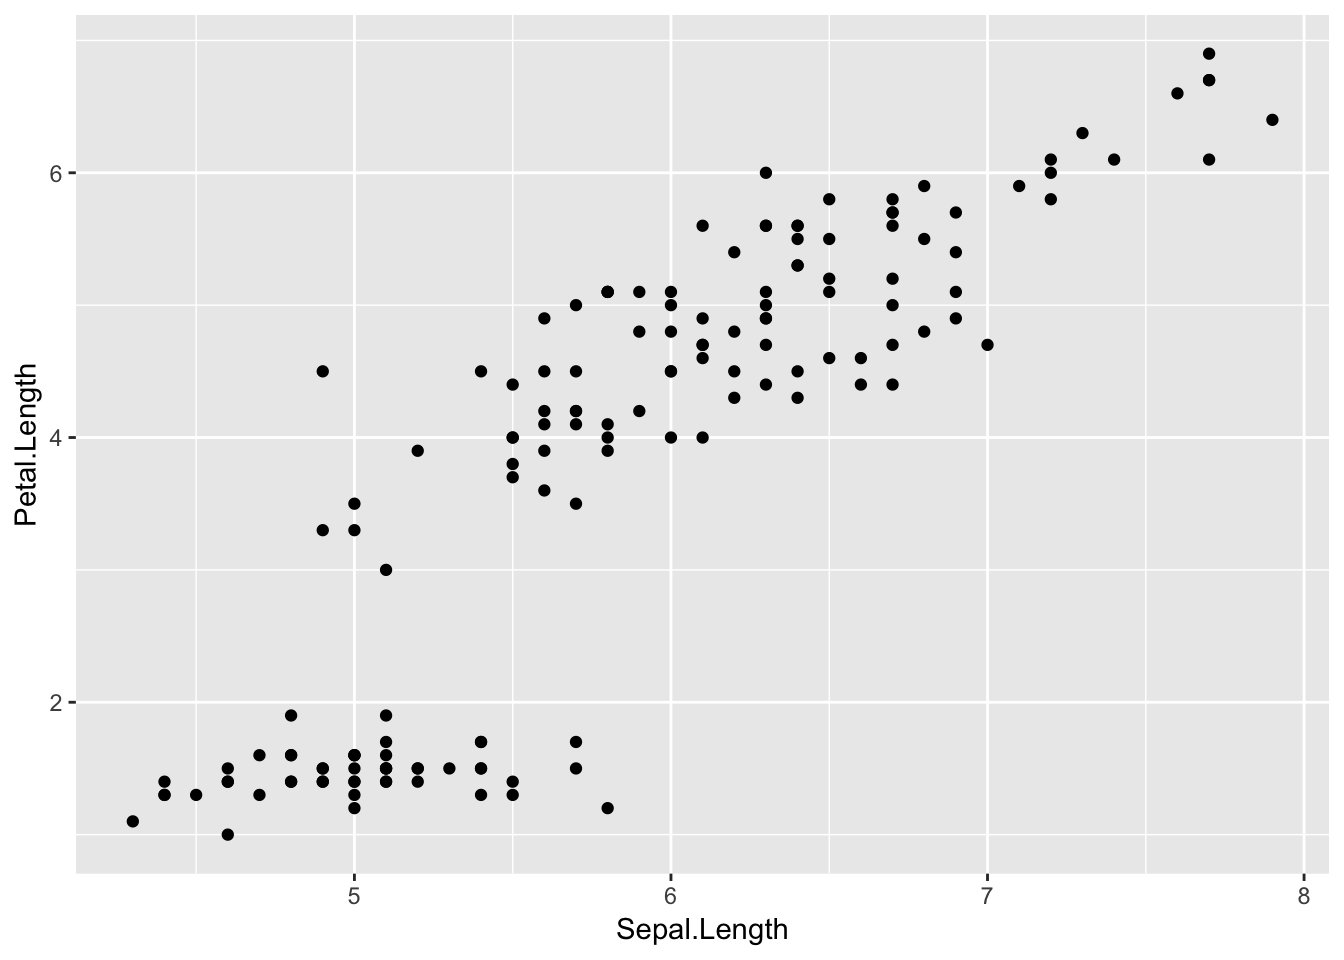
\includegraphics{Data-Analysis-for-Psychology_files/figure-latex/scatterplot_chap03-1.pdf}

\begin{Shaded}
\begin{Highlighting}[]
\NormalTok{ggplot2}\OperatorTok{::}\KeywordTok{qplot}\NormalTok{(}\DataTypeTok{data =}\NormalTok{ iris, Petal.Length, Sepal.Width)}
\end{Highlighting}
\end{Shaded}

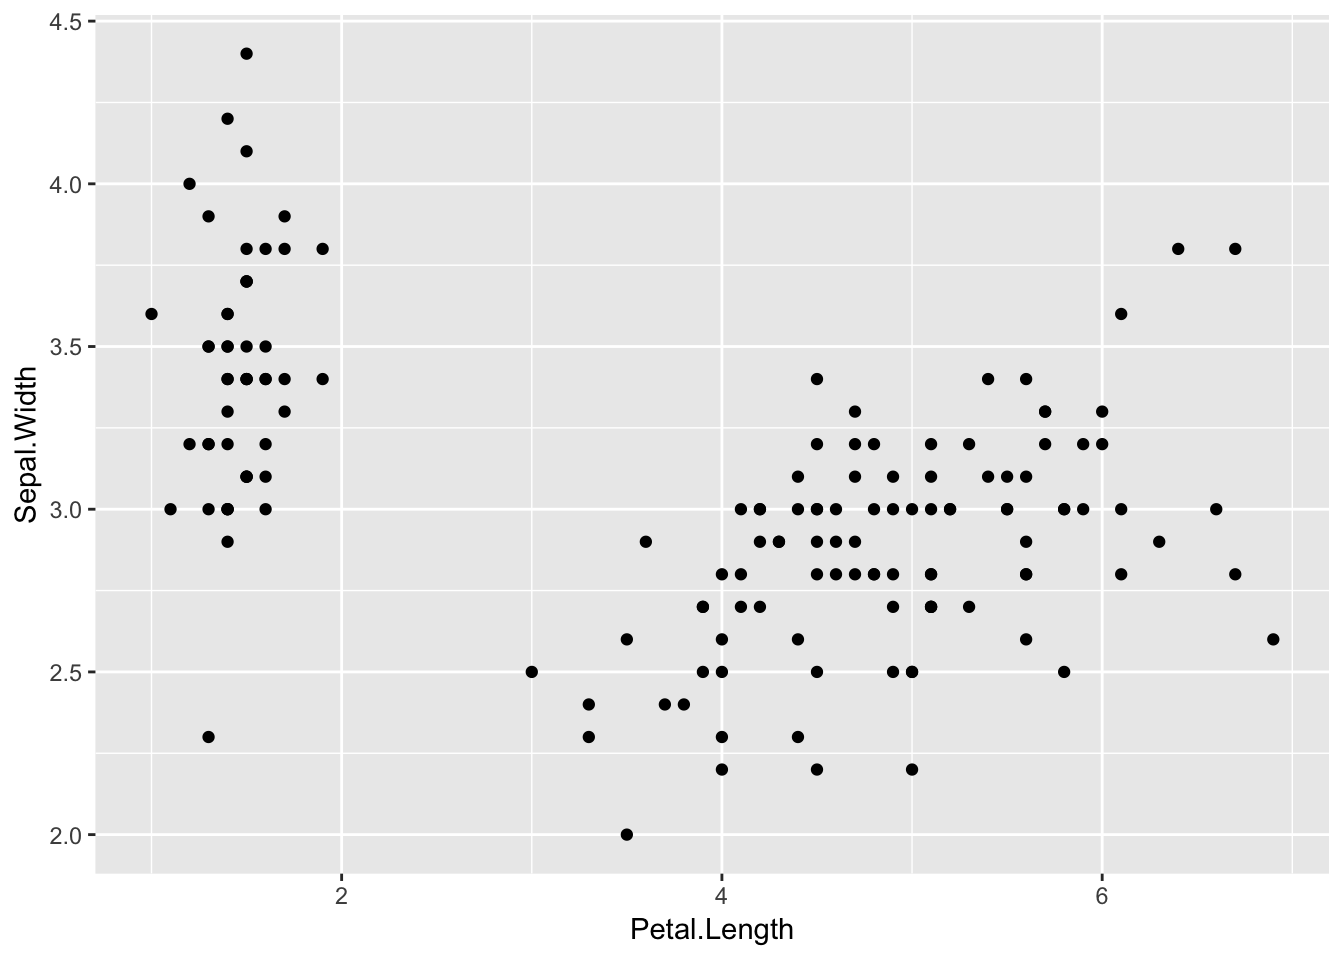
\includegraphics{Data-Analysis-for-Psychology_files/figure-latex/scatterplot_chap03-2.pdf}

\subsubsection{ピアソンの積率相関係数}

変数xと変数yの席率相関係数rは,以下の式で求められる。

\[
r = \frac{\sigma_{xy}}{\sigma_{x}\sigma_{y}}
\]

\(\sigma_{xy}\)はxとyの共分散で,\(\sigma_{xy} = \sum^n_{i=1}(x_{i}-\bar{x})(y_{i}-\bar{y})\)である(\(\bar{x}\)はxの標本平均)。\(\sigma_{x}\)と\(\sigma_{y}\)はxとyそれぞれの標本標準偏差である。

変数Xと変数Yの相関係数rが
\(r > 0\)のとき,「変数Xと変数Yの間に正の相関関係がある」という。\(r < 0\)のときは,「変数Xと変数Yの間に負の相関関係がある」という。正の相関関係は,一方の変数の量が増えればもう一方の変数も増えるという関係のことを言う。負の相関関係は,一方が増えればもう一方が減るという関係のことを言う。

試しに,様々な相関係数の場合の散布図を見てみよう。

\begin{Shaded}
\begin{Highlighting}[]
\NormalTok{r =}\StringTok{ }\FloatTok{0.5} \CommentTok{#rの値を変えてプロットを確認してみよう}
\NormalTok{x =}\StringTok{ }\KeywordTok{rnorm}\NormalTok{(}\DecValTok{1000}\NormalTok{, }\DataTypeTok{mean=}\DecValTok{0}\NormalTok{, }\DataTypeTok{sd=}\DecValTok{1}\NormalTok{) }\CommentTok{#平均0,標準偏差1の正規分布から1,000個乱数を作る。}
\NormalTok{y =}\StringTok{ }\NormalTok{r}\OperatorTok{*}\NormalTok{x }\OperatorTok{+}\StringTok{ }\KeywordTok{sqrt}\NormalTok{(}\DecValTok{1}\OperatorTok{-}\NormalTok{r}\OperatorTok{^}\DecValTok{2}\NormalTok{)}\OperatorTok{*}\KeywordTok{rnorm}\NormalTok{(}\DecValTok{1000}\NormalTok{, }\DataTypeTok{mean=}\DecValTok{0}\NormalTok{, }\DataTypeTok{sd=}\DecValTok{1}\NormalTok{)}
\KeywordTok{cor.test}\NormalTok{(x, y)}
\end{Highlighting}
\end{Shaded}

\begin{verbatim}
## 
##  Pearson's product-moment correlation
## 
## data:  x and y
## t = 20.361, df = 998, p-value < 2.2e-16
## alternative hypothesis: true correlation is not equal to 0
## 95 percent confidence interval:
##  0.4964219 0.5841188
## sample estimates:
##      cor 
## 0.541743
\end{verbatim}

\begin{Shaded}
\begin{Highlighting}[]
\KeywordTok{qplot}\NormalTok{(x, y) }\OperatorTok{+}\StringTok{ }\KeywordTok{ggtitle}\NormalTok{(r)}
\end{Highlighting}
\end{Shaded}

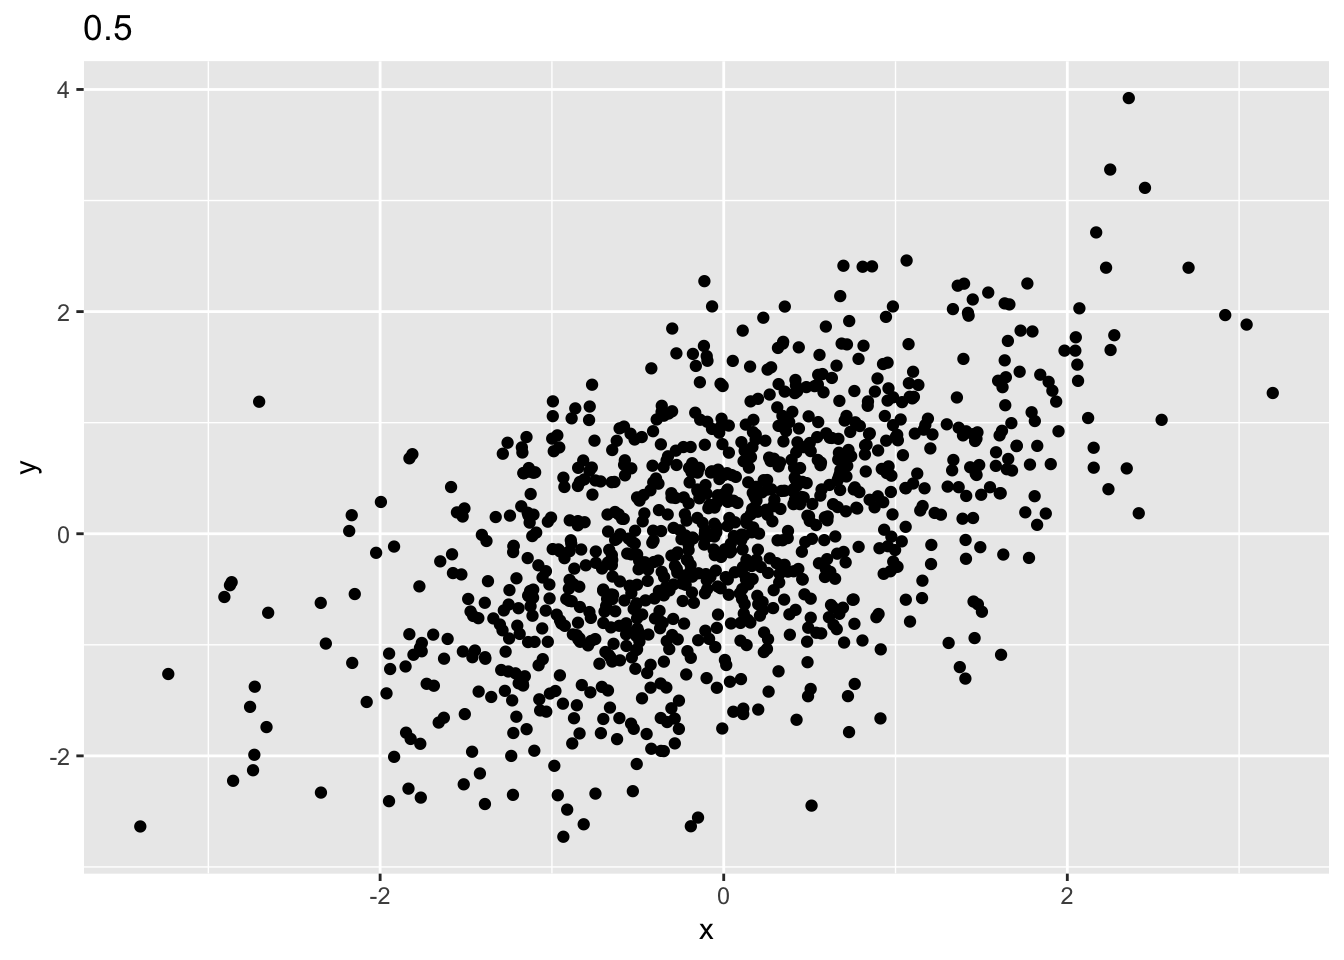
\includegraphics{Data-Analysis-for-Psychology_files/figure-latex/cor_data_chap03-1.pdf}

相関係数の絶対値の大きさが,その相関関係の強さを意味する。一般的に, .20
\textless{} \textbar{}r\textbar{} \textless{} .40 くらいを「
弱い相関」,.40 \textless{} \textbar{}r\textbar{} \textless{}
.70くらいを「強い相関」, \textbar{}r\textbar{} \textgreater{} .70
くらいを「かなり強い相関」と表現する。

しかし,分野にもよるし,相関係数の強弱の判断はいわば「研究者の主観」である(社会調査においては,\textbar{}r\textbar{}
=
.10でも意味のある相関として扱う場合もある)。また,相関係数が有意かどうかにもよる。

Rでは,相関係数を求めるための関数cor.test()がある。相関を求めたい二つの変数を入れれば,その相関係数と相関係数の有意性検定(母集団の相関係数がゼロから離れているか)の結果が出力される。

\begin{Shaded}
\begin{Highlighting}[]
\KeywordTok{cor.test}\NormalTok{(iris}\OperatorTok{$}\NormalTok{Sepal.Length, iris}\OperatorTok{$}\NormalTok{Petal.Length)}
\end{Highlighting}
\end{Shaded}

\begin{verbatim}
## 
##  Pearson's product-moment correlation
## 
## data:  iris$Sepal.Length and iris$Petal.Length
## t = 21.646, df = 148, p-value < 2.2e-16
## alternative hypothesis: true correlation is not equal to 0
## 95 percent confidence interval:
##  0.8270363 0.9055080
## sample estimates:
##       cor 
## 0.8717538
\end{verbatim}

\begin{Shaded}
\begin{Highlighting}[]
\KeywordTok{cor.test}\NormalTok{(iris}\OperatorTok{$}\NormalTok{Petal.Length, iris}\OperatorTok{$}\NormalTok{Sepal.Width)}
\end{Highlighting}
\end{Shaded}

\begin{verbatim}
## 
##  Pearson's product-moment correlation
## 
## data:  iris$Petal.Length and iris$Sepal.Width
## t = -5.7684, df = 148, p-value = 4.513e-08
## alternative hypothesis: true correlation is not equal to 0
## 95 percent confidence interval:
##  -0.5508771 -0.2879499
## sample estimates:
##        cor 
## -0.4284401
\end{verbatim}

\subsubsection{スピアマンの順位相関係数}

Rでは,cor.test()関数でスピアマンの順位相関係数も求めることが出来る。オプションでmethod
=
``spearman''と入れれば良い(methodに何も指定しないとデフォルトでピアソンの積率相関係数が算出される)。

\begin{Shaded}
\begin{Highlighting}[]
\KeywordTok{cor.test}\NormalTok{(iris}\OperatorTok{$}\NormalTok{Sepal.Length, iris}\OperatorTok{$}\NormalTok{Petal.Length, }\DataTypeTok{method =} \StringTok{"spearman"}\NormalTok{)}
\end{Highlighting}
\end{Shaded}

\begin{verbatim}
## 
##  Spearman's rank correlation rho
## 
## data:  iris$Sepal.Length and iris$Petal.Length
## S = 66429, p-value < 2.2e-16
## alternative hypothesis: true rho is not equal to 0
## sample estimates:
##       rho 
## 0.8818981
\end{verbatim}

\begin{Shaded}
\begin{Highlighting}[]
\KeywordTok{cor.test}\NormalTok{(iris}\OperatorTok{$}\NormalTok{Petal.Length, iris}\OperatorTok{$}\NormalTok{Sepal.Width, }\DataTypeTok{method =} \StringTok{"spearman"}\NormalTok{)}
\end{Highlighting}
\end{Shaded}

\begin{verbatim}
## 
##  Spearman's rank correlation rho
## 
## data:  iris$Petal.Length and iris$Sepal.Width
## S = 736640, p-value = 0.0001154
## alternative hypothesis: true rho is not equal to 0
## sample estimates:
##        rho 
## -0.3096351
\end{verbatim}

\subsubsection{外れ値の影響}

データに極端な値がある場合,ピアソンの相関係数では結果が歪む恐れがある。

\begin{Shaded}
\begin{Highlighting}[]
\KeywordTok{library}\NormalTok{(MASS) }\CommentTok{#MASSパッケージにあるサンプルデータAnimalsを使う}
\KeywordTok{head}\NormalTok{(Animals) }\CommentTok{#28種の動物の体重と脳重量のデータ}
\end{Highlighting}
\end{Shaded}

\begin{verbatim}
##                     body brain
## Mountain beaver     1.35   8.1
## Cow               465.00 423.0
## Grey wolf          36.33 119.5
## Goat               27.66 115.0
## Guinea pig          1.04   5.5
## Dipliodocus     11700.00  50.0
\end{verbatim}

\begin{Shaded}
\begin{Highlighting}[]
\KeywordTok{qplot}\NormalTok{(}\DataTypeTok{data=}\NormalTok{Animals, body, brain)}
\end{Highlighting}
\end{Shaded}

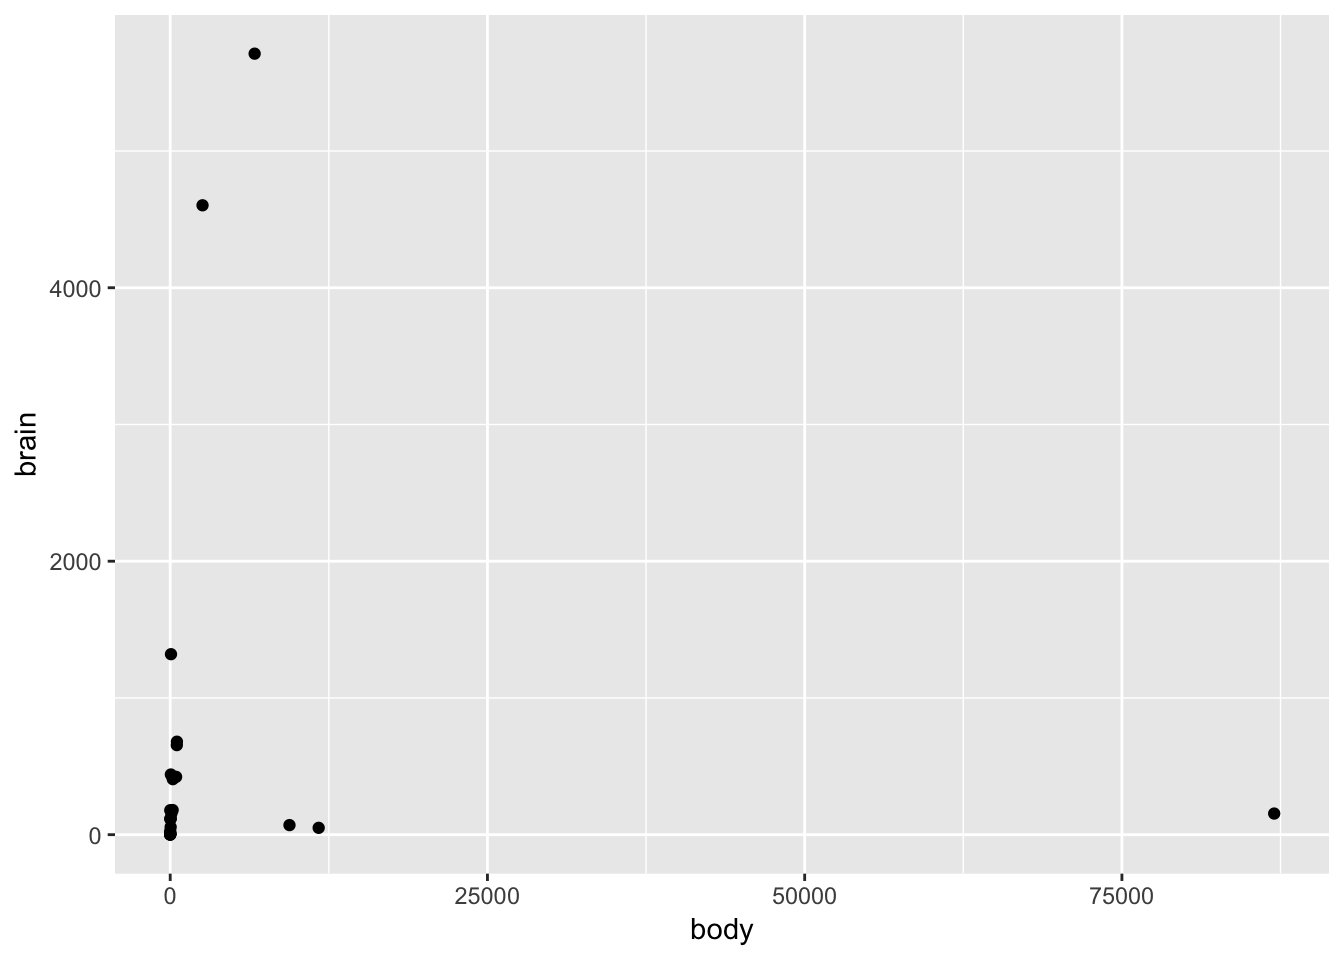
\includegraphics{Data-Analysis-for-Psychology_files/figure-latex/outlier_chap03-1.pdf}

\begin{Shaded}
\begin{Highlighting}[]
\KeywordTok{cor.test}\NormalTok{(Animals}\OperatorTok{$}\NormalTok{body, Animals}\OperatorTok{$}\NormalTok{brain) }\CommentTok{#Pearsonの相関係数を求める}
\end{Highlighting}
\end{Shaded}

\begin{verbatim}
## 
##  Pearson's product-moment correlation
## 
## data:  Animals$body and Animals$brain
## t = -0.027235, df = 26, p-value = 0.9785
## alternative hypothesis: true correlation is not equal to 0
## 95 percent confidence interval:
##  -0.3776655  0.3684700
## sample estimates:
##          cor 
## -0.005341163
\end{verbatim}

極端に体重が大きくかつ脳重量の小さい種が影響している。

\begin{itemize}
\tightlist
\item
  相関係数を鵜呑みにするのではなく,必ず散布図を確認する。
\item
  対処法としては,

  \begin{itemize}
  \tightlist
  \item
    外れ値を除去して相関を見る。
  \item
    スピアマンの順位相関係数を見る。順位相関はデータを順位(1位,2位,3位,\ldots{})に変換して相関係数を出したものであり,これにより外れ値の影響が調整される。
  \end{itemize}
\end{itemize}

\begin{Shaded}
\begin{Highlighting}[]
\NormalTok{Animal_}\DecValTok{2}\NormalTok{ =}\StringTok{ }\NormalTok{dplyr}\OperatorTok{::}\KeywordTok{filter}\NormalTok{(Animals, body }\OperatorTok{<}\StringTok{ }\DecValTok{10000}\NormalTok{)}
\KeywordTok{qplot}\NormalTok{(}\DataTypeTok{data=}\NormalTok{Animal_}\DecValTok{2}\NormalTok{, body, brain)}
\end{Highlighting}
\end{Shaded}

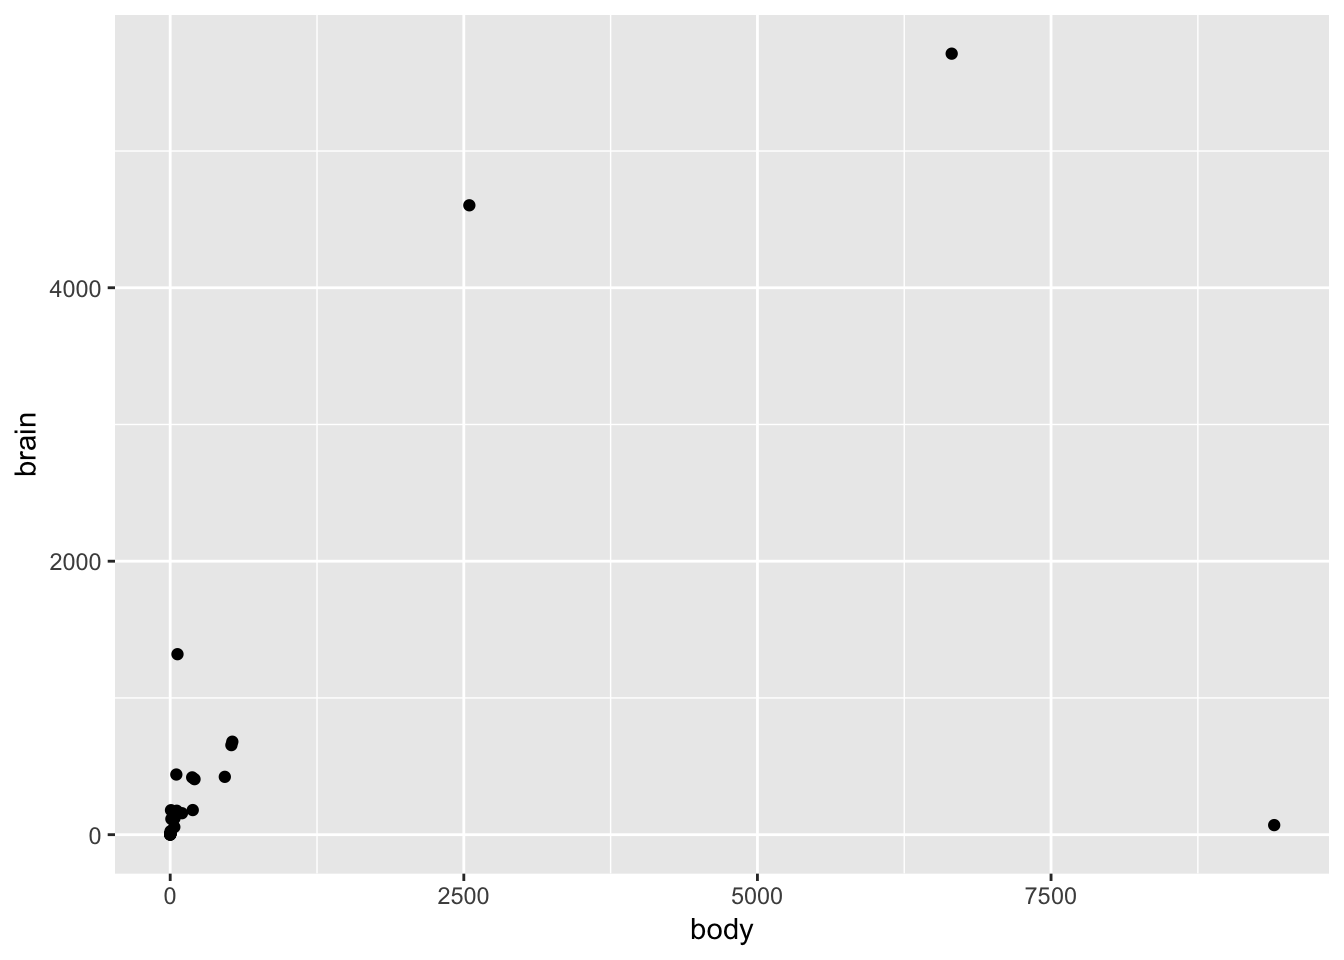
\includegraphics{Data-Analysis-for-Psychology_files/figure-latex/outlier2_chap03-1.pdf}

\begin{Shaded}
\begin{Highlighting}[]
\KeywordTok{cor.test}\NormalTok{(Animal_}\DecValTok{2}\OperatorTok{$}\NormalTok{body, Animal_}\DecValTok{2}\OperatorTok{$}\NormalTok{brain) }\CommentTok{#Pearsonの相関係数を求める}
\end{Highlighting}
\end{Shaded}

\begin{verbatim}
## 
##  Pearson's product-moment correlation
## 
## data:  Animal_2$body and Animal_2$brain
## t = 2.8764, df = 24, p-value = 0.008308
## alternative hypothesis: true correlation is not equal to 0
## 95 percent confidence interval:
##  0.1479923 0.7471395
## sample estimates:
##       cor 
## 0.5063195
\end{verbatim}

\begin{Shaded}
\begin{Highlighting}[]
\KeywordTok{cor.test}\NormalTok{(Animals}\OperatorTok{$}\NormalTok{body, Animals}\OperatorTok{$}\NormalTok{brain, }\DataTypeTok{method=}\StringTok{"spearman"}\NormalTok{) }\CommentTok{#外れ値除去前のデータでSpearmanの相関係数を求める}
\end{Highlighting}
\end{Shaded}

\begin{verbatim}
## 
##  Spearman's rank correlation rho
## 
## data:  Animals$body and Animals$brain
## S = 1036.6, p-value = 1.813e-05
## alternative hypothesis: true rho is not equal to 0
## sample estimates:
##       rho 
## 0.7162994
\end{verbatim}

\subsubsection{相関関係と因果関係}

因果関係とは,原因と結果の関係である(X -\textgreater{}
Y:XがYの原因である)。相関関係はあくまで,一方の変数の増減ともう一方の変数の増減に関係があることである(X
\textless{}-\textgreater{} Y)。

XとYとの間の相関係数を求めて有意な相関があったとしても,両者の間に因果関係があるとは結論付けることはできない。

因果関係がないのに相関関係があるように見える例(中室・津川(2017)より)。

\begin{itemize}
\tightlist
\item
  アイスクリームの売上が高いと水死者が増える(第3の要因:「暑さ」という共通の要因)。\\
\item
  警察官が多い街ほど犯罪が多い(逆の因果:犯罪が多いところにたくさん警察官を配置している)。\\
\item
  大気中の二酸化炭素量が増えるほど海賊が増える(偶然)。
\end{itemize}

\subsection{データの可視化}\label{-1}

平均値や相関係数を計算する前に,グラフを作ってデータの分布を確かめる習慣をつけよう(データの可視化)。

以下では,Rのggplot2パッケージを使って代表的なグラフを作成してみた。ggplot2を使ったグラフの作成方法については覚える必要はない。あくまで,データを可視化する手段として,どのようなグラフがよく使われるかを例として挙げる。

\subsubsection{散布図}

\begin{Shaded}
\begin{Highlighting}[]
\NormalTok{p <-}\StringTok{ }\KeywordTok{ggplot}\NormalTok{(}\DataTypeTok{data =}\NormalTok{ iris, }\KeywordTok{aes}\NormalTok{(}\DataTypeTok{x=}\NormalTok{Sepal.Length, }\DataTypeTok{y=}\NormalTok{Petal.Length)) }\OperatorTok{+}\StringTok{ }
\StringTok{      }\KeywordTok{geom_point}\NormalTok{()}
\NormalTok{p}
\end{Highlighting}
\end{Shaded}

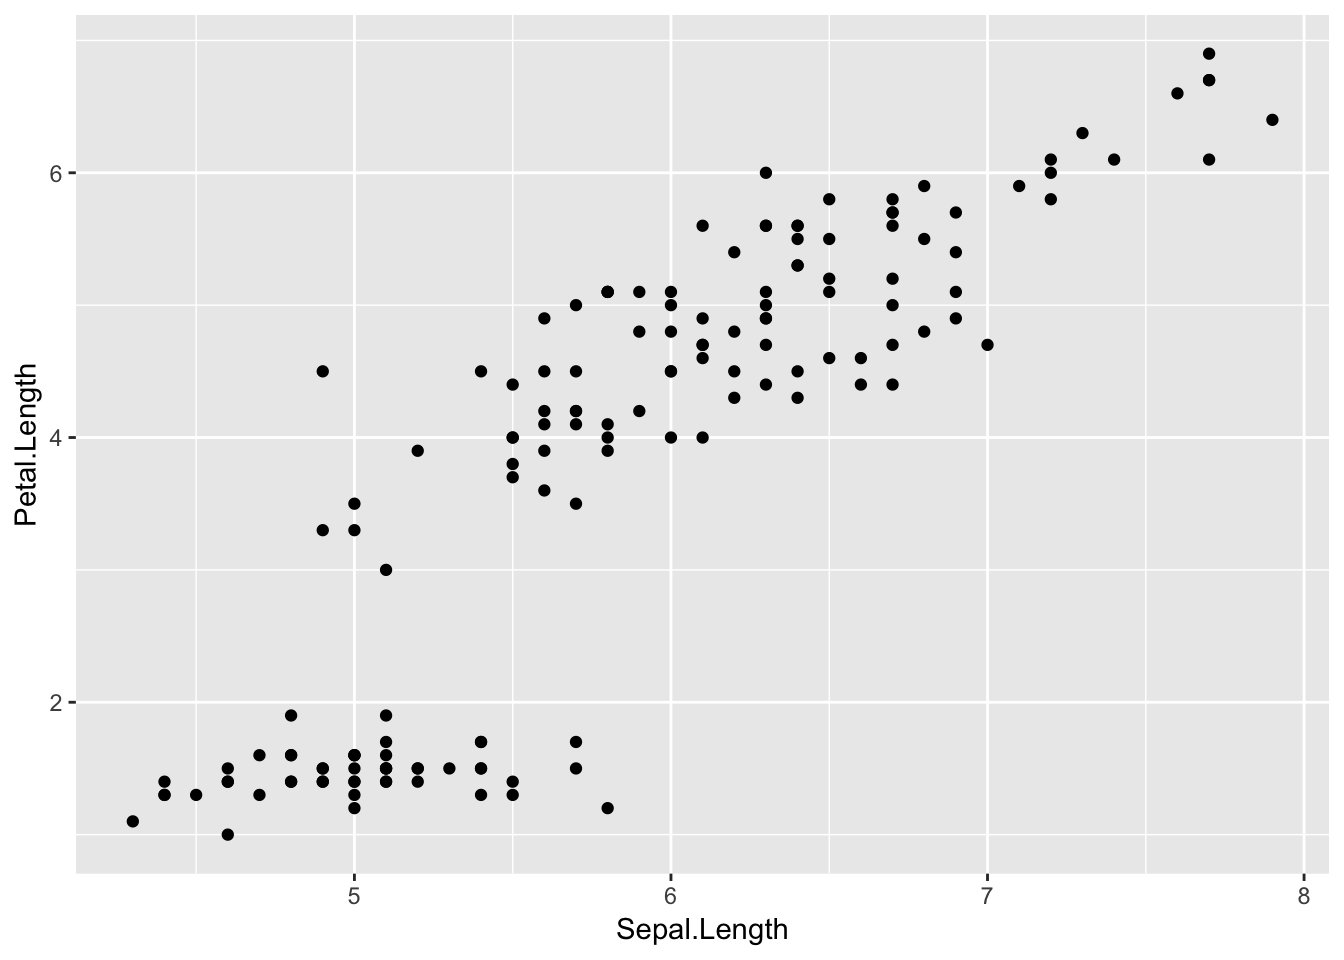
\includegraphics{Data-Analysis-for-Psychology_files/figure-latex/ggplot2_scatterplot_chap03-1.pdf}

\subsubsection{ヒストグラム}

\begin{Shaded}
\begin{Highlighting}[]
\NormalTok{p <-}\StringTok{ }\KeywordTok{ggplot}\NormalTok{(}\DataTypeTok{data =}\NormalTok{ cars, }\KeywordTok{aes}\NormalTok{(}\DataTypeTok{x=}\NormalTok{dist)) }\OperatorTok{+}\StringTok{ }
\StringTok{      }\KeywordTok{geom_histogram}\NormalTok{()}
\NormalTok{p}
\end{Highlighting}
\end{Shaded}

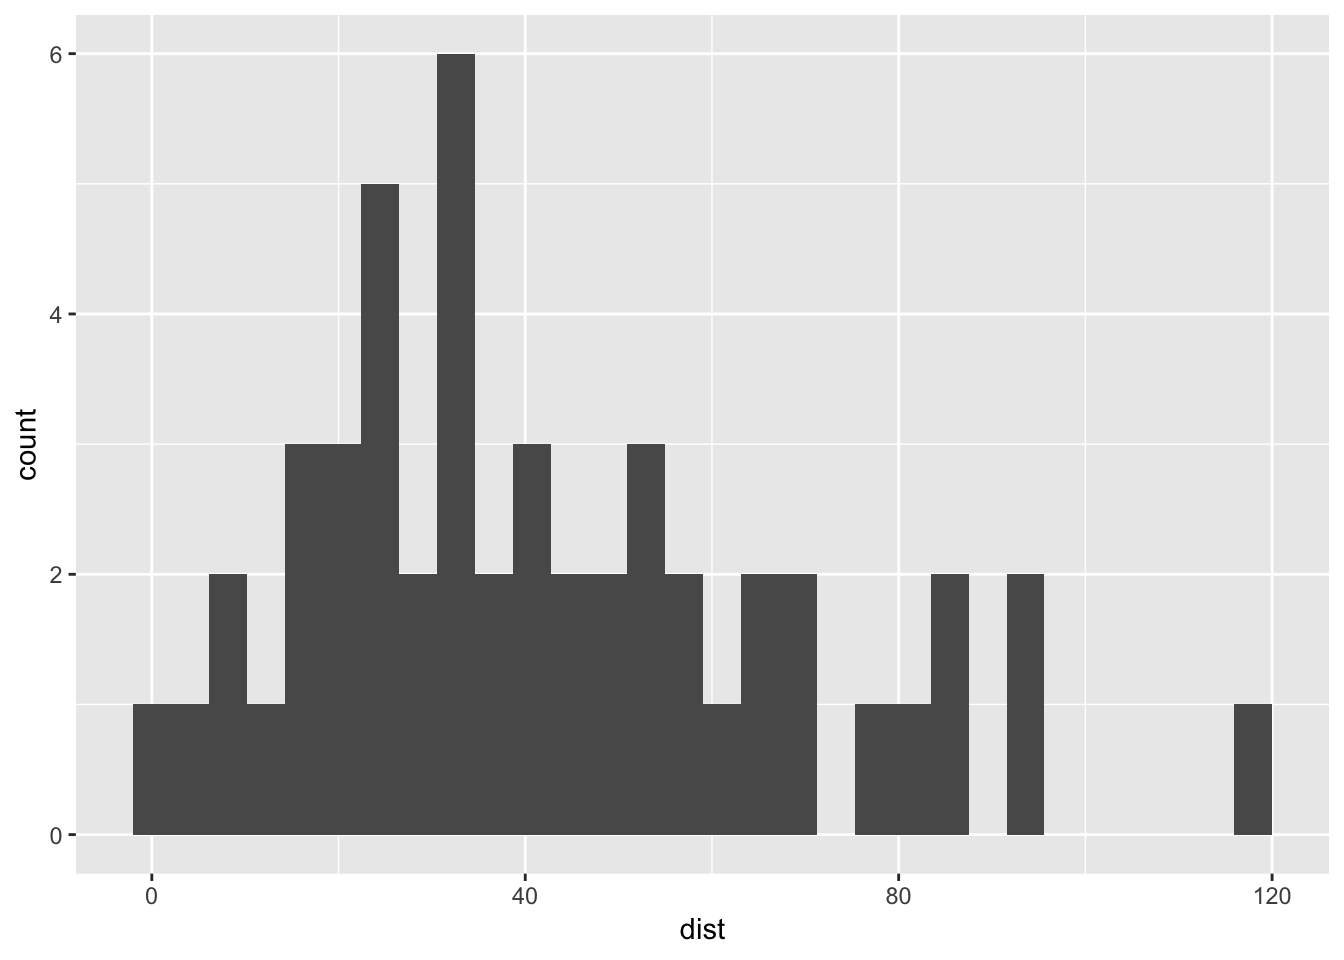
\includegraphics{Data-Analysis-for-Psychology_files/figure-latex/ggplot2_histogram_chap03-1.pdf}

\subsubsection{箱ひげ図}

最小値,第一分位点,中央値,第三分位点,最大値を示す(外れ値は点で示される)。

\begin{Shaded}
\begin{Highlighting}[]
\NormalTok{p <-}\StringTok{ }\KeywordTok{ggplot}\NormalTok{(}\DataTypeTok{data =}\NormalTok{ InsectSprays, }\KeywordTok{aes}\NormalTok{(}\DataTypeTok{x=}\NormalTok{spray, }\DataTypeTok{y=}\NormalTok{count)) }\OperatorTok{+}\StringTok{ }
\StringTok{      }\KeywordTok{geom_boxplot}\NormalTok{()}
\NormalTok{p}
\end{Highlighting}
\end{Shaded}

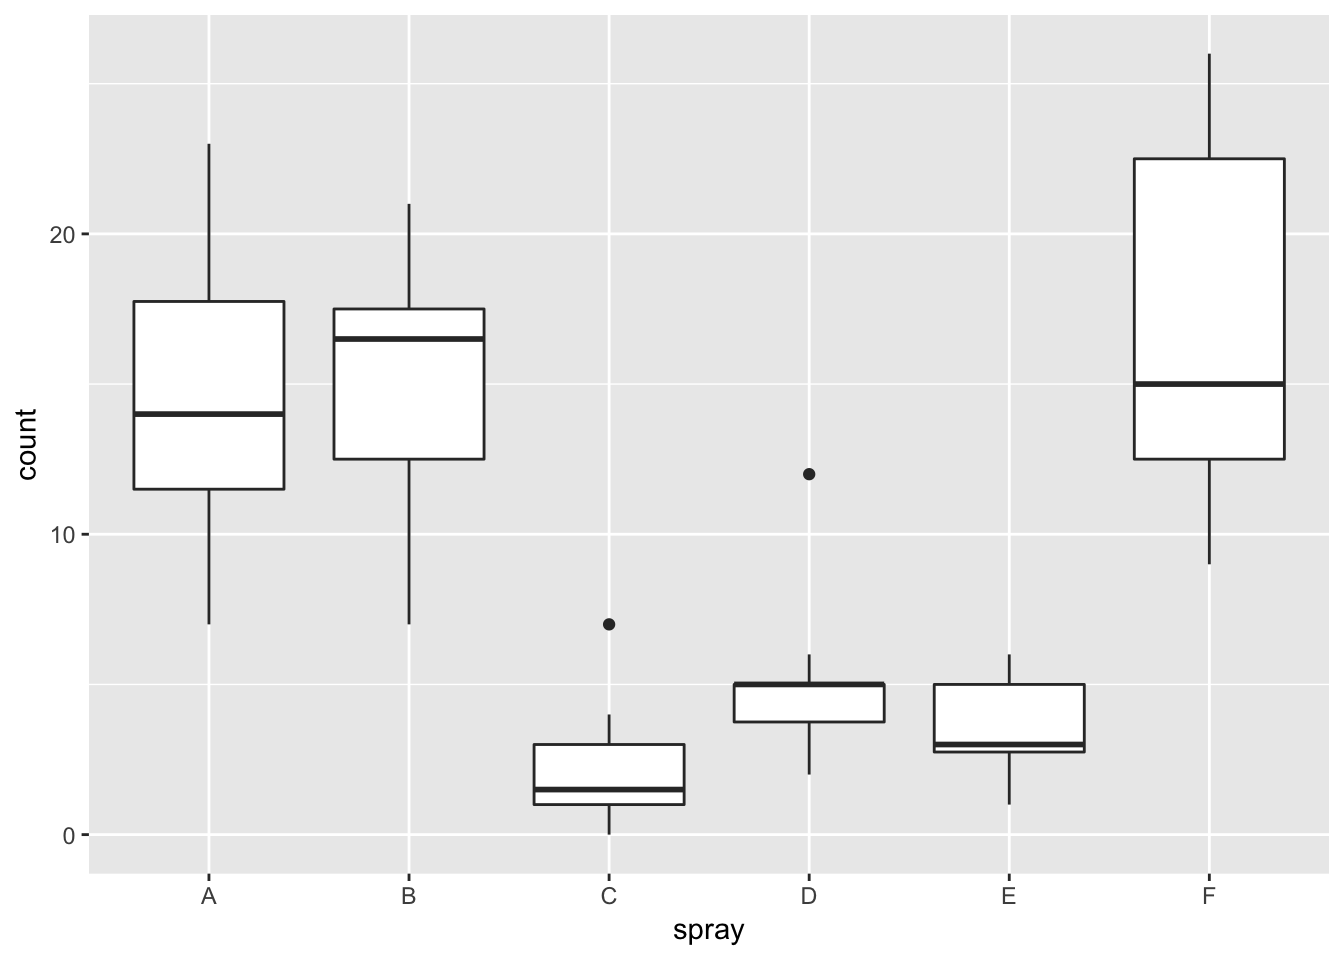
\includegraphics{Data-Analysis-for-Psychology_files/figure-latex/ggplot2_boxplot_chap03-1.pdf}

\subsubsection{棒グラフ}

\begin{Shaded}
\begin{Highlighting}[]
\CommentTok{#サンプルデータをつくる: あやめの種ごとのがくの幅の平均}
\NormalTok{iris_mean <-}\StringTok{ }\KeywordTok{data.frame}\NormalTok{(}
    \DataTypeTok{Sepecies  =} \KeywordTok{c}\NormalTok{(}\StringTok{"setosa"}\NormalTok{, }\StringTok{"versicolor"}\NormalTok{, }\StringTok{"virginica"}\NormalTok{), }
    \DataTypeTok{Width =} \KeywordTok{c}\NormalTok{(}\FloatTok{3.43}\NormalTok{, }\FloatTok{2.77}\NormalTok{, }\FloatTok{2.97}\NormalTok{)}
\NormalTok{)}

\NormalTok{p <-}\StringTok{ }\KeywordTok{ggplot}\NormalTok{(}\DataTypeTok{data =}\NormalTok{ iris_mean, }\KeywordTok{aes}\NormalTok{(}\DataTypeTok{x=}\NormalTok{Sepecies, }\DataTypeTok{y=}\NormalTok{Width)) }\OperatorTok{+}\StringTok{ }
\StringTok{      }\KeywordTok{geom_bar}\NormalTok{(}\DataTypeTok{stat =} \StringTok{"identity"}\NormalTok{)}
\NormalTok{p}
\end{Highlighting}
\end{Shaded}

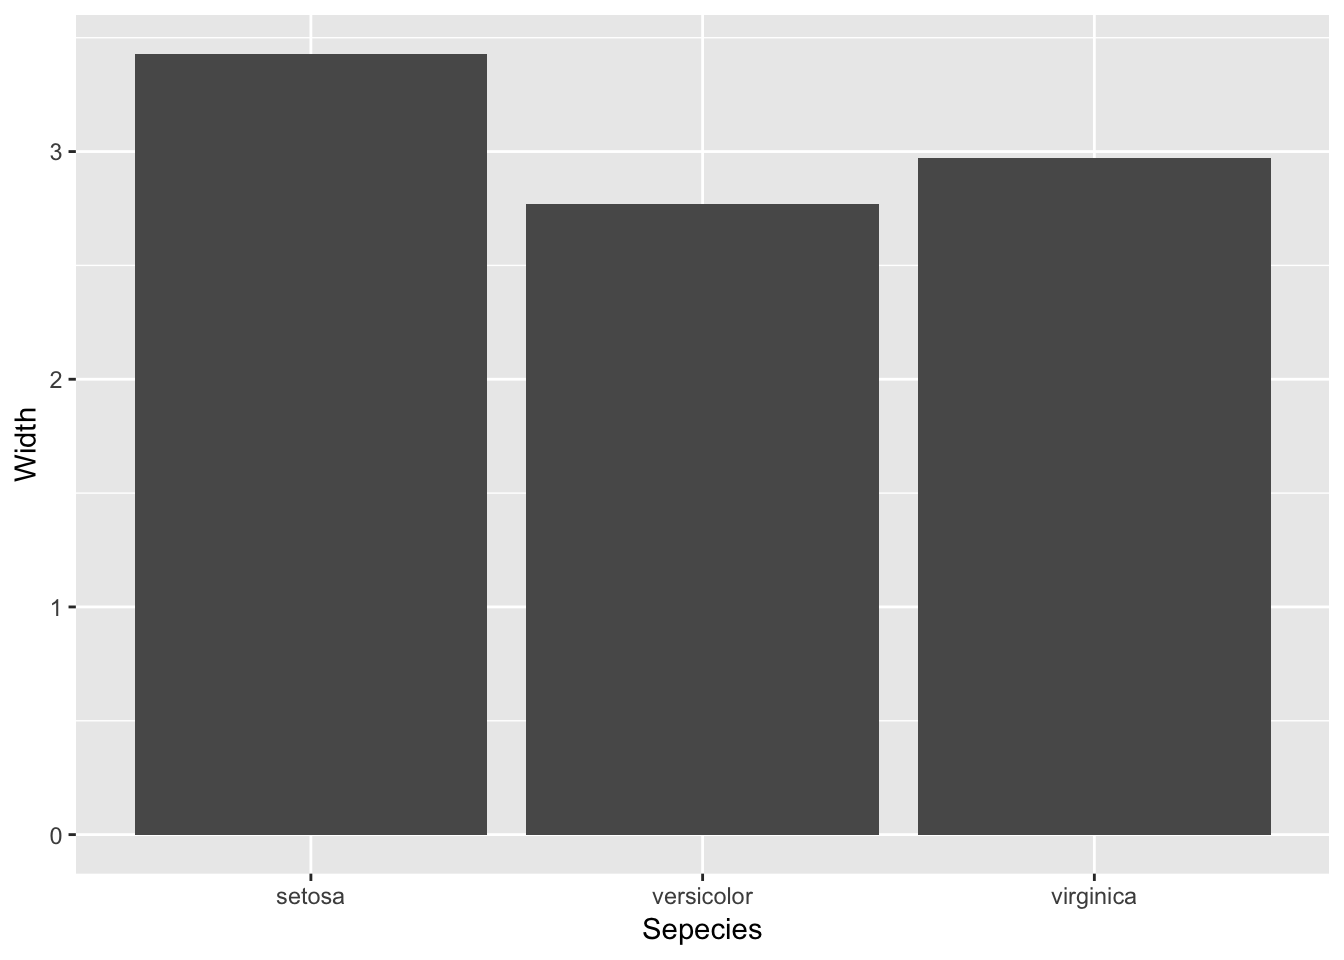
\includegraphics{Data-Analysis-for-Psychology_files/figure-latex/ggplot2_barplot_chap03-1.pdf}

\subsubsection{折れ線グラフ}

\begin{Shaded}
\begin{Highlighting}[]
\CommentTok{#サンプルデータをつくる: 10日間の気温の変化}
\NormalTok{temperature <-}\StringTok{ }\KeywordTok{data.frame}\NormalTok{(}
    \DataTypeTok{Days  =} \DecValTok{1}\OperatorTok{:}\DecValTok{10}\NormalTok{, }
    \DataTypeTok{Celsius =} \KeywordTok{c}\NormalTok{(}\FloatTok{17.2}\NormalTok{, }\FloatTok{17.5}\NormalTok{, }\FloatTok{18.1}\NormalTok{, }\FloatTok{18.8}\NormalTok{, }\FloatTok{19.0}\NormalTok{, }\FloatTok{19.2}\NormalTok{, }\FloatTok{19.7}\NormalTok{, }\FloatTok{20.2}\NormalTok{, }\FloatTok{20.5}\NormalTok{, }\FloatTok{20.1}\NormalTok{)}
\NormalTok{)}

\NormalTok{p <-}\StringTok{ }\KeywordTok{ggplot}\NormalTok{(}\DataTypeTok{data =}\NormalTok{ temperature, }\KeywordTok{aes}\NormalTok{(}\DataTypeTok{x=}\NormalTok{Days, }\DataTypeTok{y=}\NormalTok{Celsius)) }\OperatorTok{+}\StringTok{ }
\StringTok{      }\KeywordTok{geom_line}\NormalTok{()}
\NormalTok{p}
\end{Highlighting}
\end{Shaded}

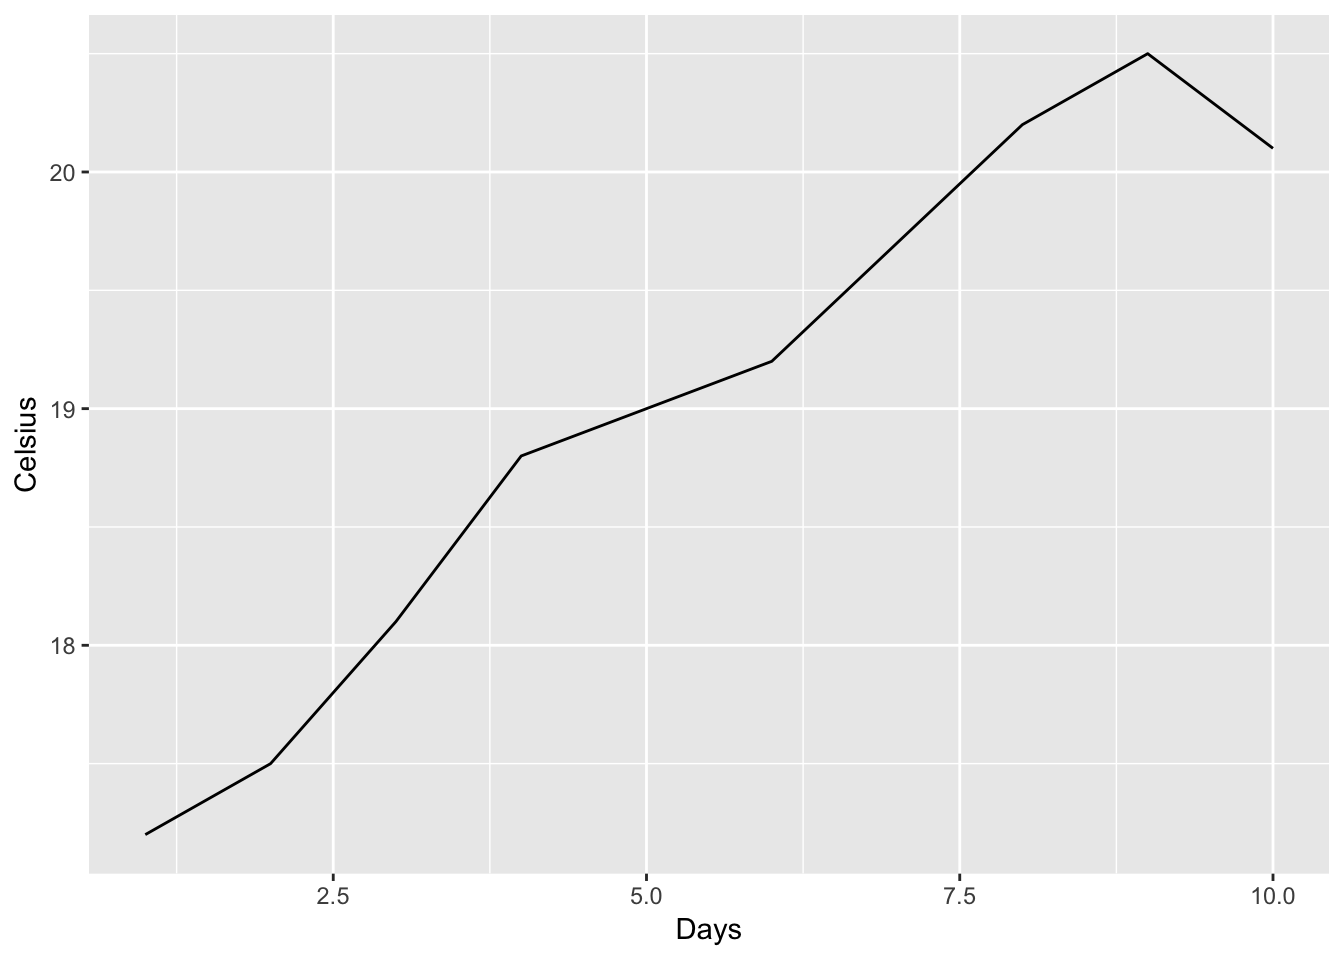
\includegraphics{Data-Analysis-for-Psychology_files/figure-latex/ggplot2_lineplot_chap03-1.pdf}

\subsubsection{応用}

\begin{Shaded}
\begin{Highlighting}[]
\NormalTok{p <-}\StringTok{ }\KeywordTok{ggplot}\NormalTok{(}\DataTypeTok{data =}\NormalTok{ iris, }\KeywordTok{aes}\NormalTok{(}\DataTypeTok{x=}\NormalTok{Sepal.Length, }\DataTypeTok{y=}\NormalTok{Petal.Length)) }\OperatorTok{+}\StringTok{ }
\StringTok{      }\KeywordTok{geom_point}\NormalTok{(}\KeywordTok{aes}\NormalTok{(}\DataTypeTok{shape =}\NormalTok{ Species))}
\NormalTok{p <-}\StringTok{ }\NormalTok{p }\OperatorTok{+}\StringTok{ }\KeywordTok{xlab}\NormalTok{(}\StringTok{"Length of Sepal"}\NormalTok{) }\OperatorTok{+}\StringTok{ }\KeywordTok{ylab}\NormalTok{(}\StringTok{"Length of Petal"}\NormalTok{) }
\NormalTok{p}
\end{Highlighting}
\end{Shaded}

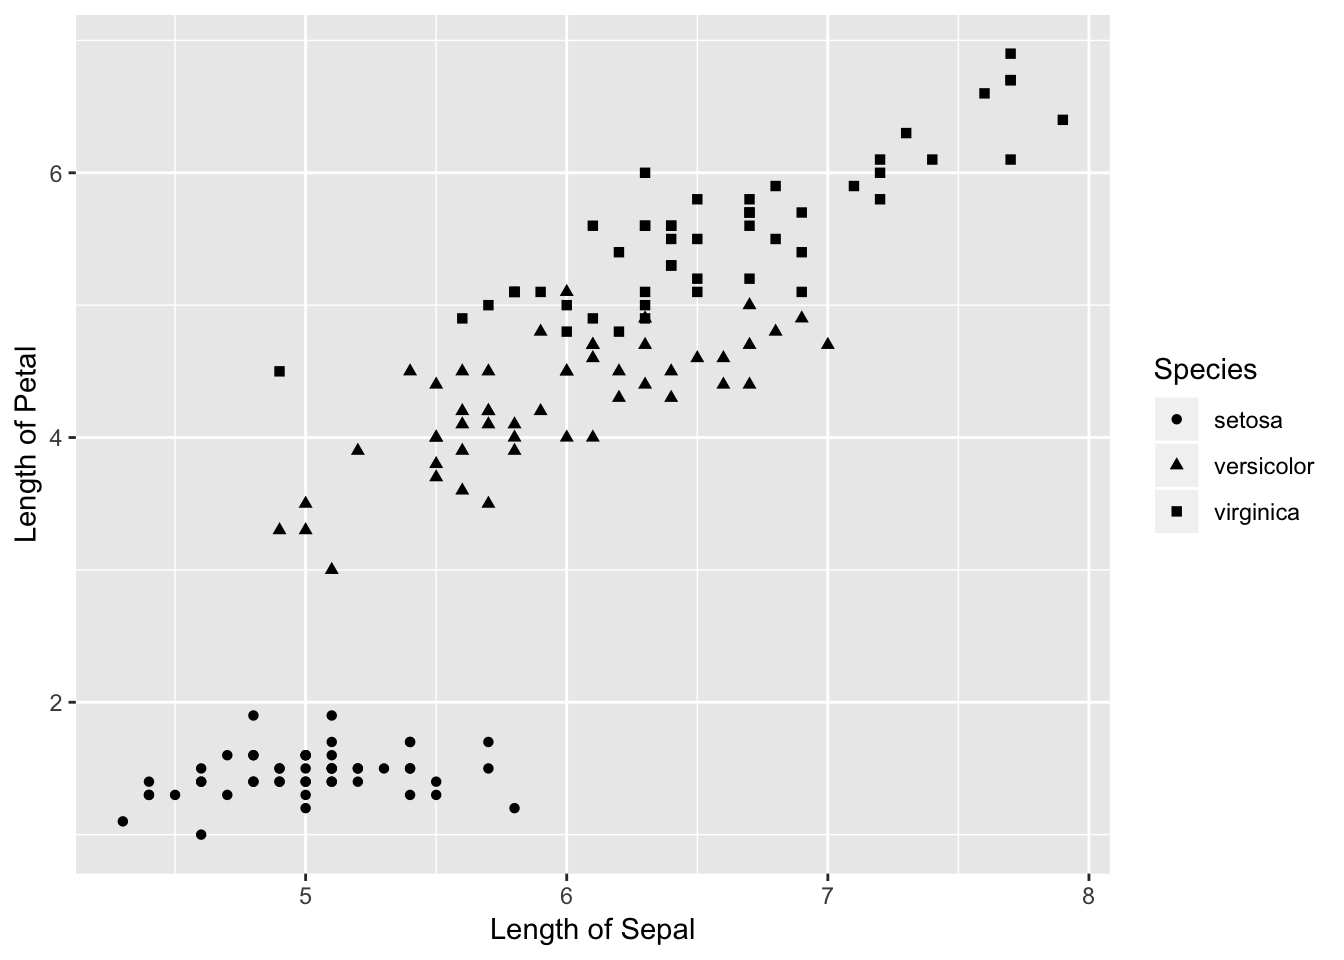
\includegraphics{Data-Analysis-for-Psychology_files/figure-latex/ggplot2_scatterplot2_chap03-1.pdf}

\begin{Shaded}
\begin{Highlighting}[]
\NormalTok{p <-}\StringTok{ }\KeywordTok{ggplot}\NormalTok{(}\DataTypeTok{data =}\NormalTok{ iris, }\KeywordTok{aes}\NormalTok{(}\DataTypeTok{x=}\NormalTok{Sepal.Length, }\DataTypeTok{y=}\NormalTok{Petal.Length)) }\OperatorTok{+}\StringTok{ }
\StringTok{      }\KeywordTok{geom_point}\NormalTok{()}
\NormalTok{p <-}\StringTok{ }\NormalTok{p }\OperatorTok{+}\StringTok{ }\KeywordTok{facet_wrap}\NormalTok{(}\OperatorTok{~}\NormalTok{Species) }
\NormalTok{p}
\end{Highlighting}
\end{Shaded}

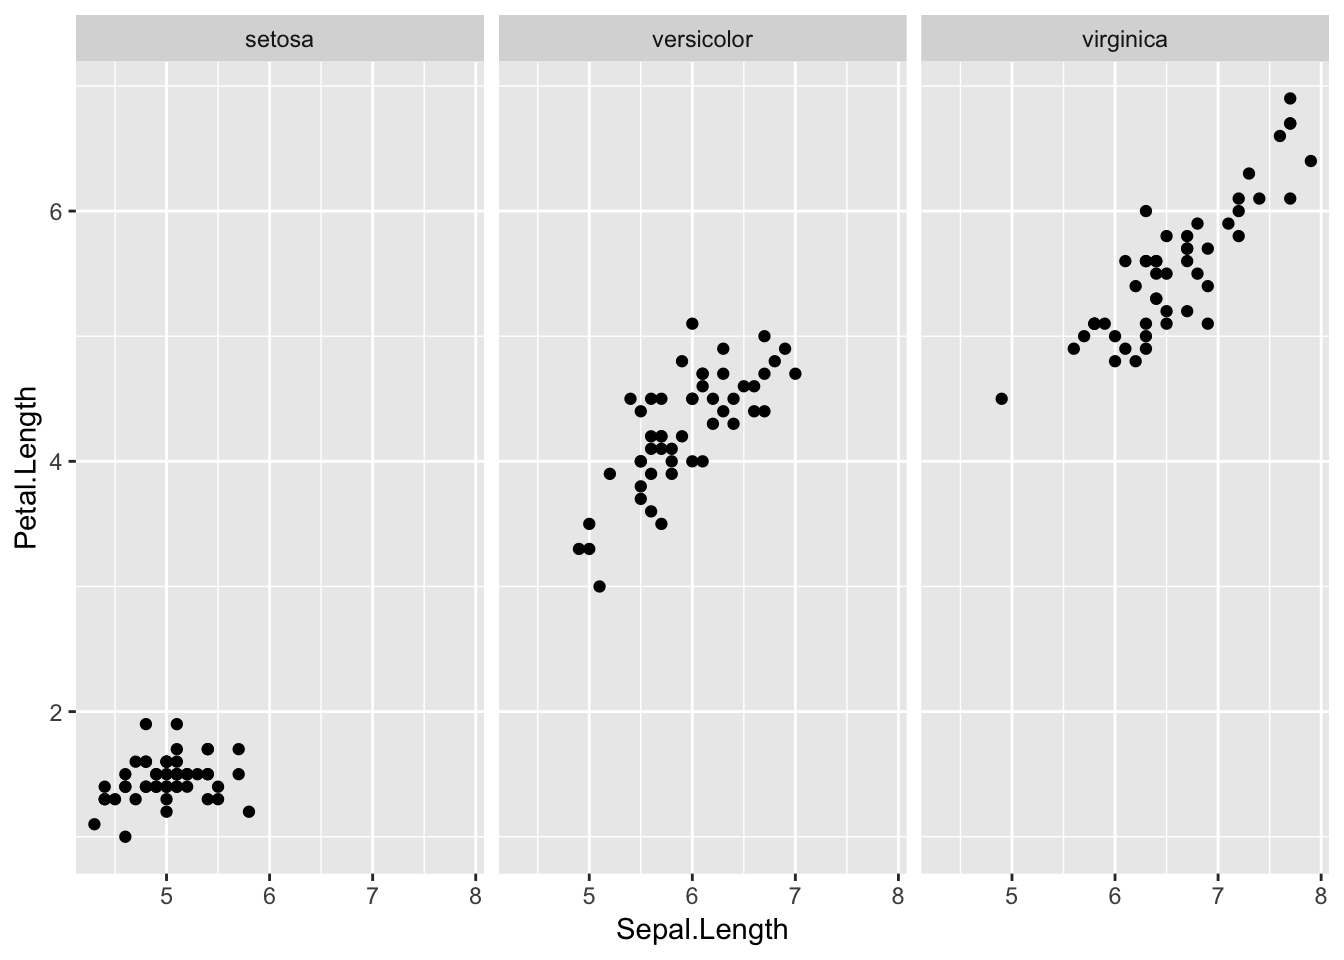
\includegraphics{Data-Analysis-for-Psychology_files/figure-latex/ggplot2_histogram2_chap03-1.pdf}

\begin{Shaded}
\begin{Highlighting}[]
\NormalTok{p <-}\StringTok{ }\KeywordTok{ggplot}\NormalTok{(}\DataTypeTok{data =}\NormalTok{ ChickWeight, }\KeywordTok{aes}\NormalTok{(}\DataTypeTok{x=}\NormalTok{weight)) }\OperatorTok{+}\StringTok{ }
\StringTok{    }\KeywordTok{geom_histogram}\NormalTok{() }\OperatorTok{+}\StringTok{ }\KeywordTok{facet_wrap}\NormalTok{(}\OperatorTok{~}\NormalTok{Diet)}
\NormalTok{p}
\end{Highlighting}
\end{Shaded}

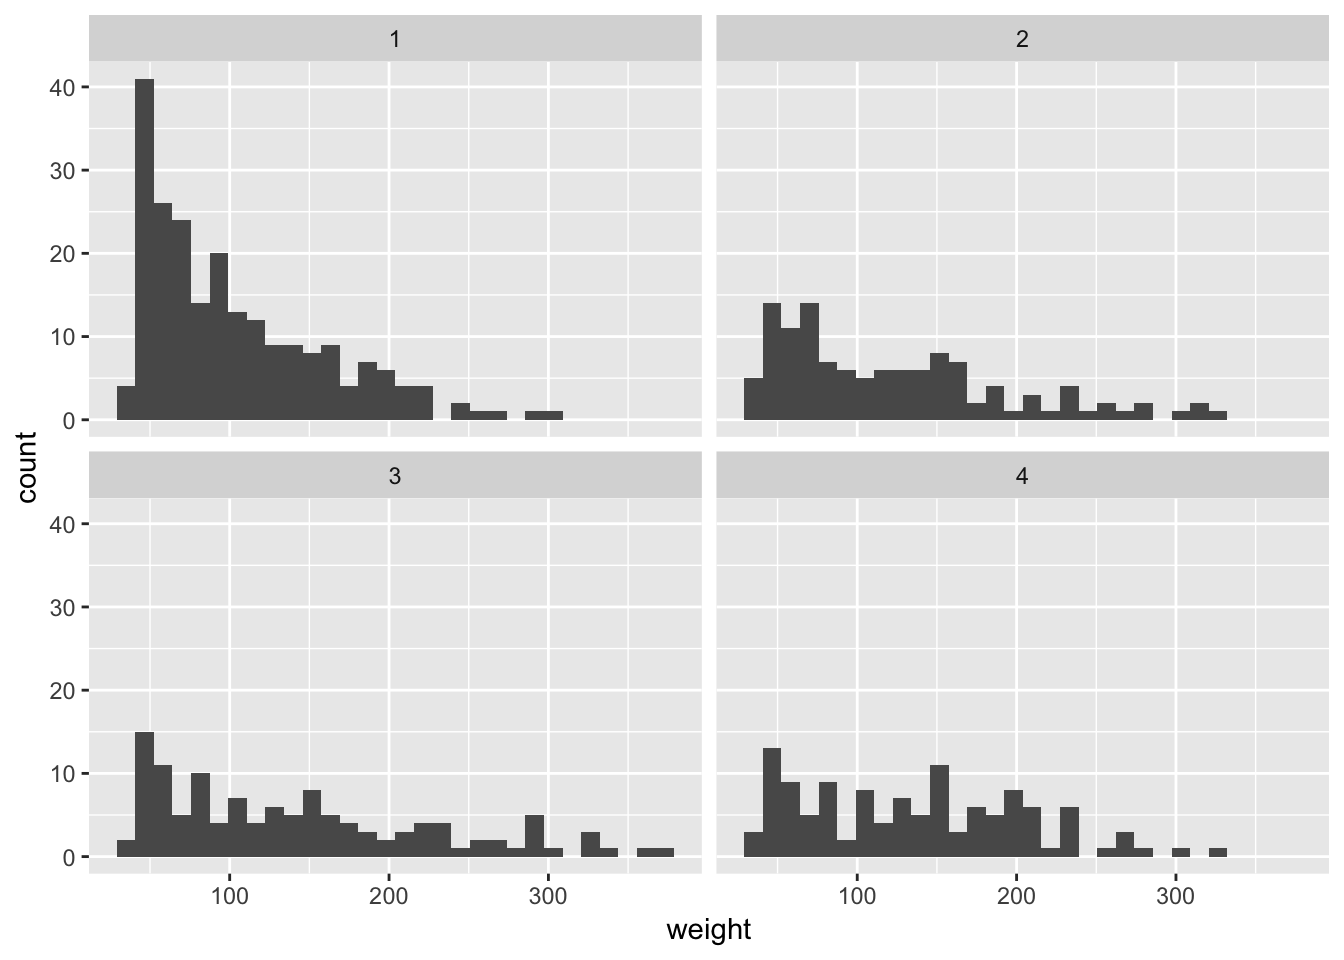
\includegraphics{Data-Analysis-for-Psychology_files/figure-latex/ggplot2_histogram2_chap03-2.pdf}

\subsubsection{簡単なグラフの作り方}

gglot2パッケージのqplot()関数でも手っ取り早くグラフを作成することが出来る。とりあえずデータの傾向を見たいだけなら,qplot()を使うのが良い。x軸もしくはy軸に指定したい変数を入れればできるので,これくらいは覚えておくと良い。
x軸とy軸に表示する変数を2つ入れれば散布図,x軸の変数1つだけならヒストグラムがデフォルトで表示される。geomでグラフの種類を指定することも可能。

\begin{Shaded}
\begin{Highlighting}[]
\KeywordTok{qplot}\NormalTok{(}\DataTypeTok{data =}\NormalTok{ iris, }\DataTypeTok{x =}\NormalTok{ Sepal.Length, }\DataTypeTok{y =}\NormalTok{ Petal.Length)}
\end{Highlighting}
\end{Shaded}

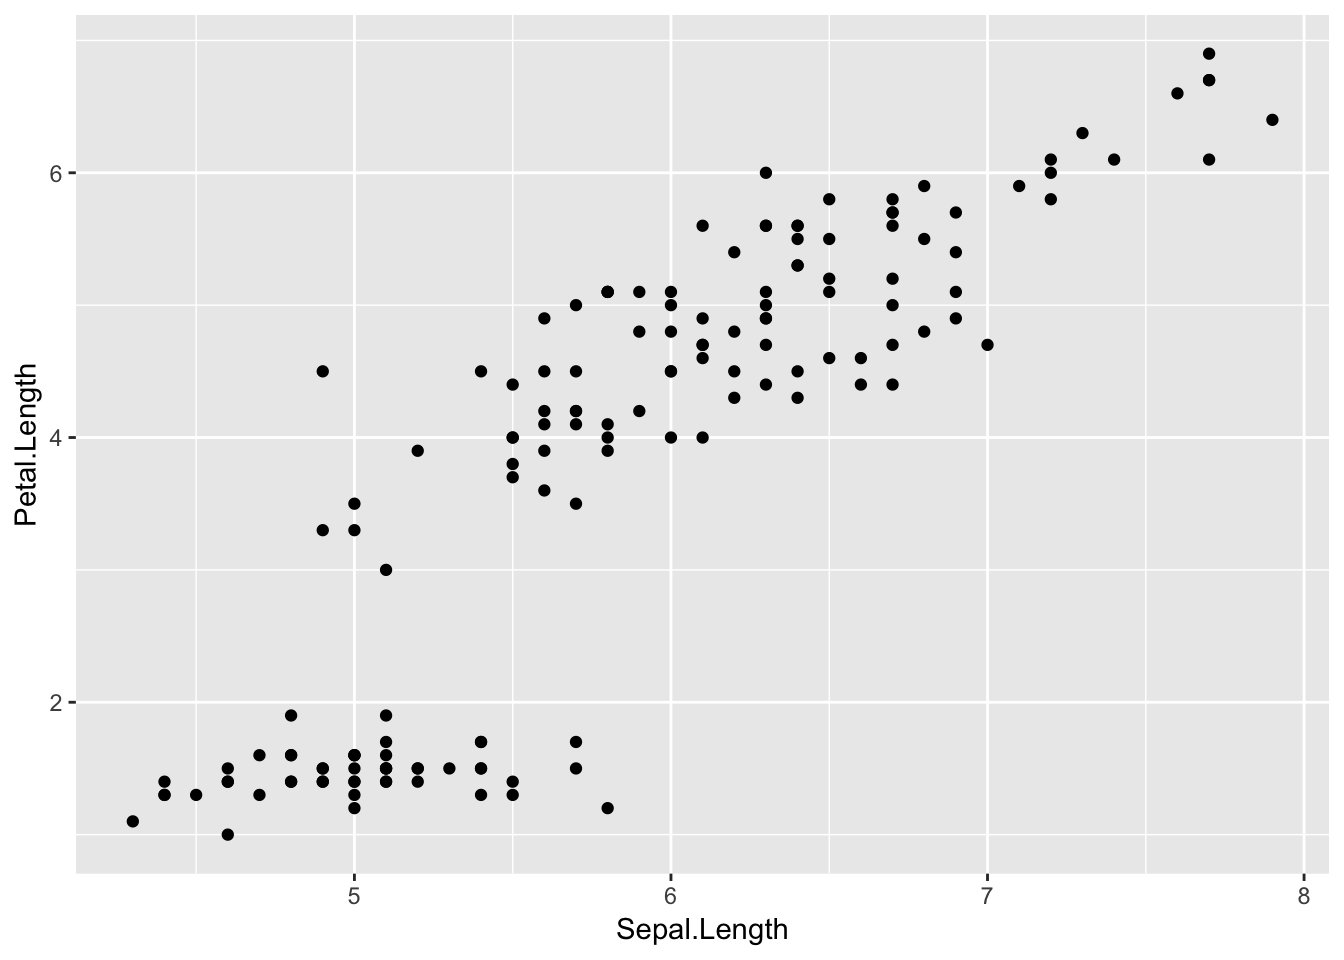
\includegraphics{Data-Analysis-for-Psychology_files/figure-latex/qplot_scatterplot_chap03-1.pdf}

\begin{Shaded}
\begin{Highlighting}[]
\KeywordTok{qplot}\NormalTok{(}\DataTypeTok{data =}\NormalTok{ ChickWeight, }\DataTypeTok{x =}\NormalTok{ weight)}
\end{Highlighting}
\end{Shaded}

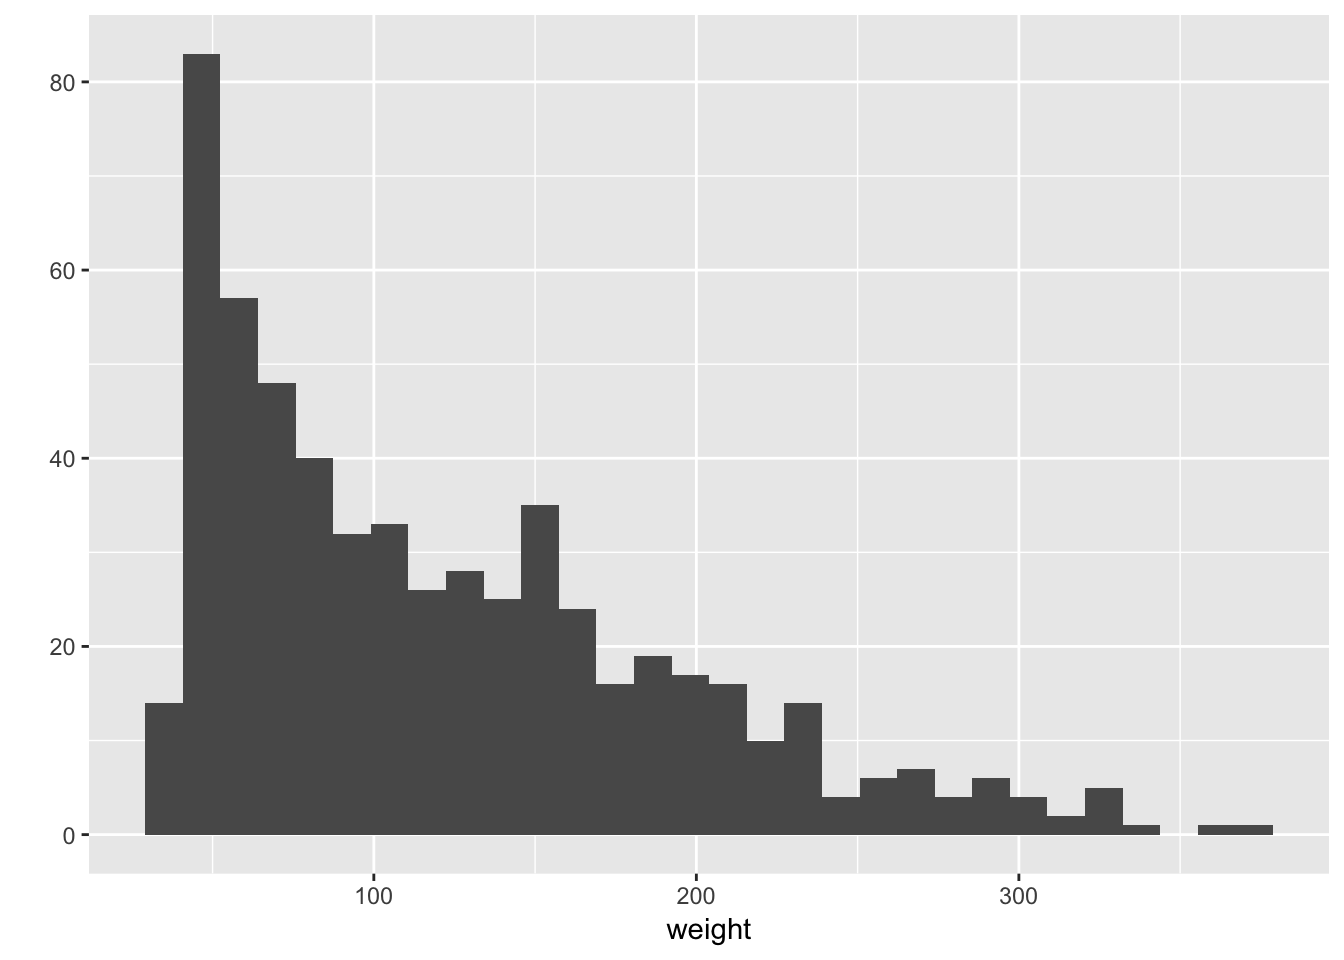
\includegraphics{Data-Analysis-for-Psychology_files/figure-latex/qplot_scatterplot_chap03-2.pdf}

\begin{Shaded}
\begin{Highlighting}[]
\KeywordTok{qplot}\NormalTok{(}\DataTypeTok{data =}\NormalTok{ InsectSprays, }\DataTypeTok{x =}\NormalTok{ spray, }\DataTypeTok{y =}\NormalTok{ count, }\DataTypeTok{geom=}\StringTok{"boxplot"}\NormalTok{)}
\end{Highlighting}
\end{Shaded}

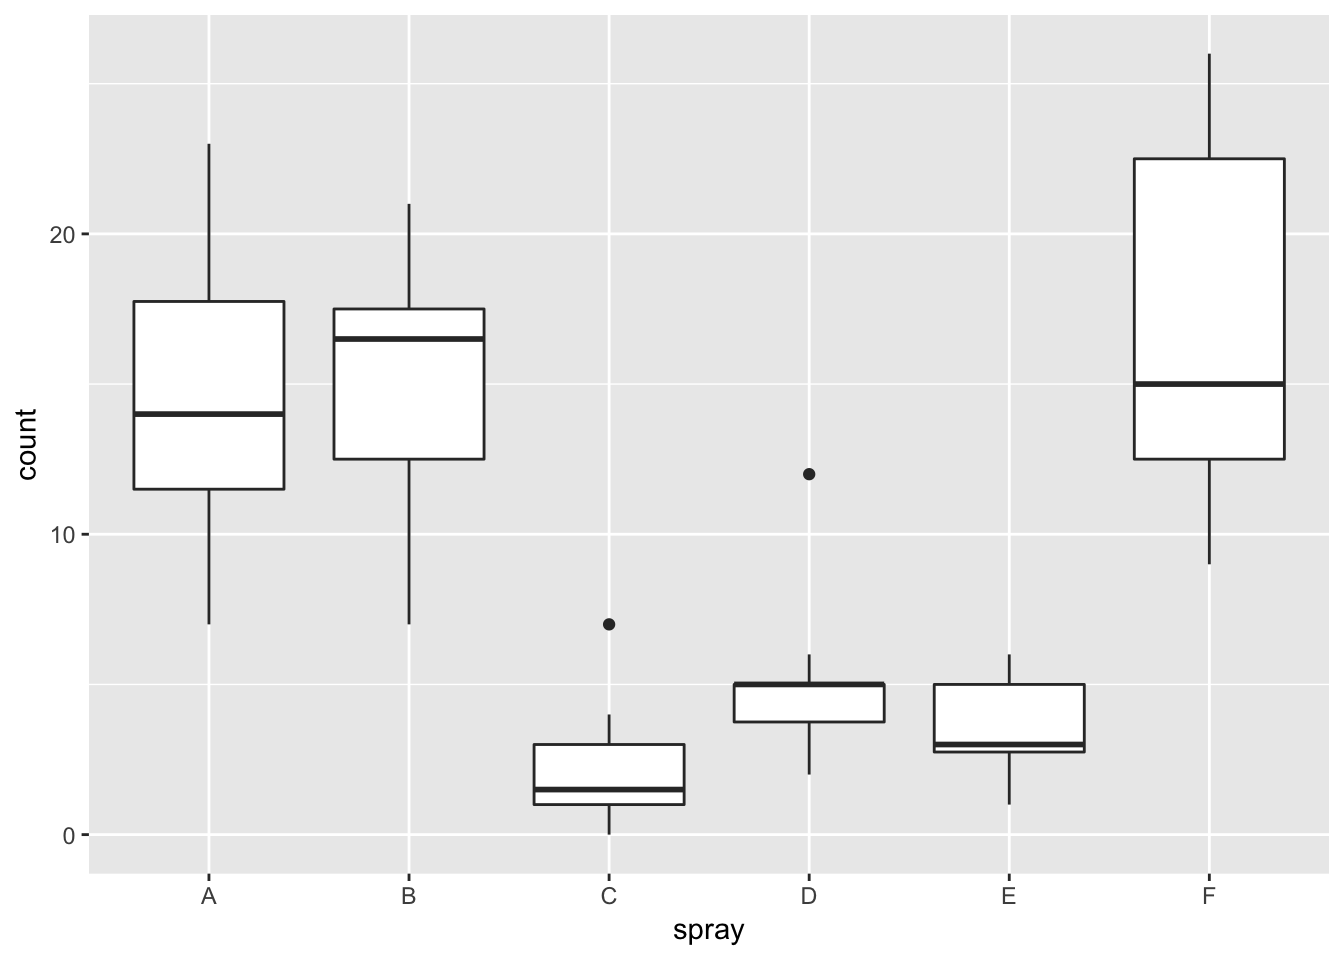
\includegraphics{Data-Analysis-for-Psychology_files/figure-latex/qplot_scatterplot_chap03-3.pdf}

gglot2パッケージがなくても,Rで標準で入っている関数でもグラフを作成することができる(ただし,見た目は良くない)。

\begin{Shaded}
\begin{Highlighting}[]
\KeywordTok{plot}\NormalTok{(iris}\OperatorTok{$}\NormalTok{Sepal.Length, iris}\OperatorTok{$}\NormalTok{Petal.Length)}
\end{Highlighting}
\end{Shaded}

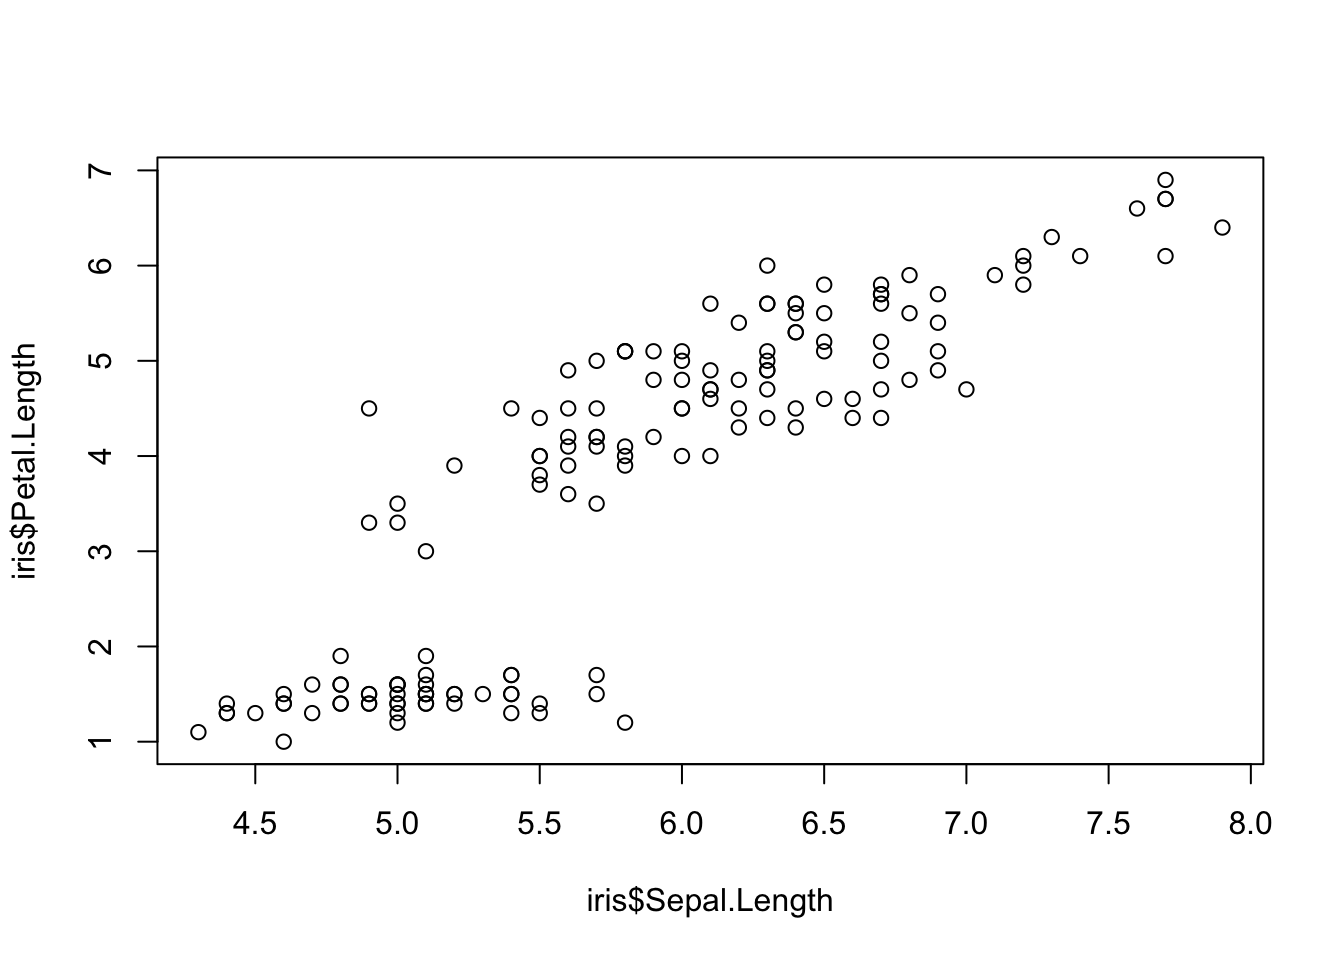
\includegraphics{Data-Analysis-for-Psychology_files/figure-latex/plot_chap03-1.pdf}

\begin{Shaded}
\begin{Highlighting}[]
\KeywordTok{hist}\NormalTok{(ChickWeight}\OperatorTok{$}\NormalTok{weight)}
\end{Highlighting}
\end{Shaded}

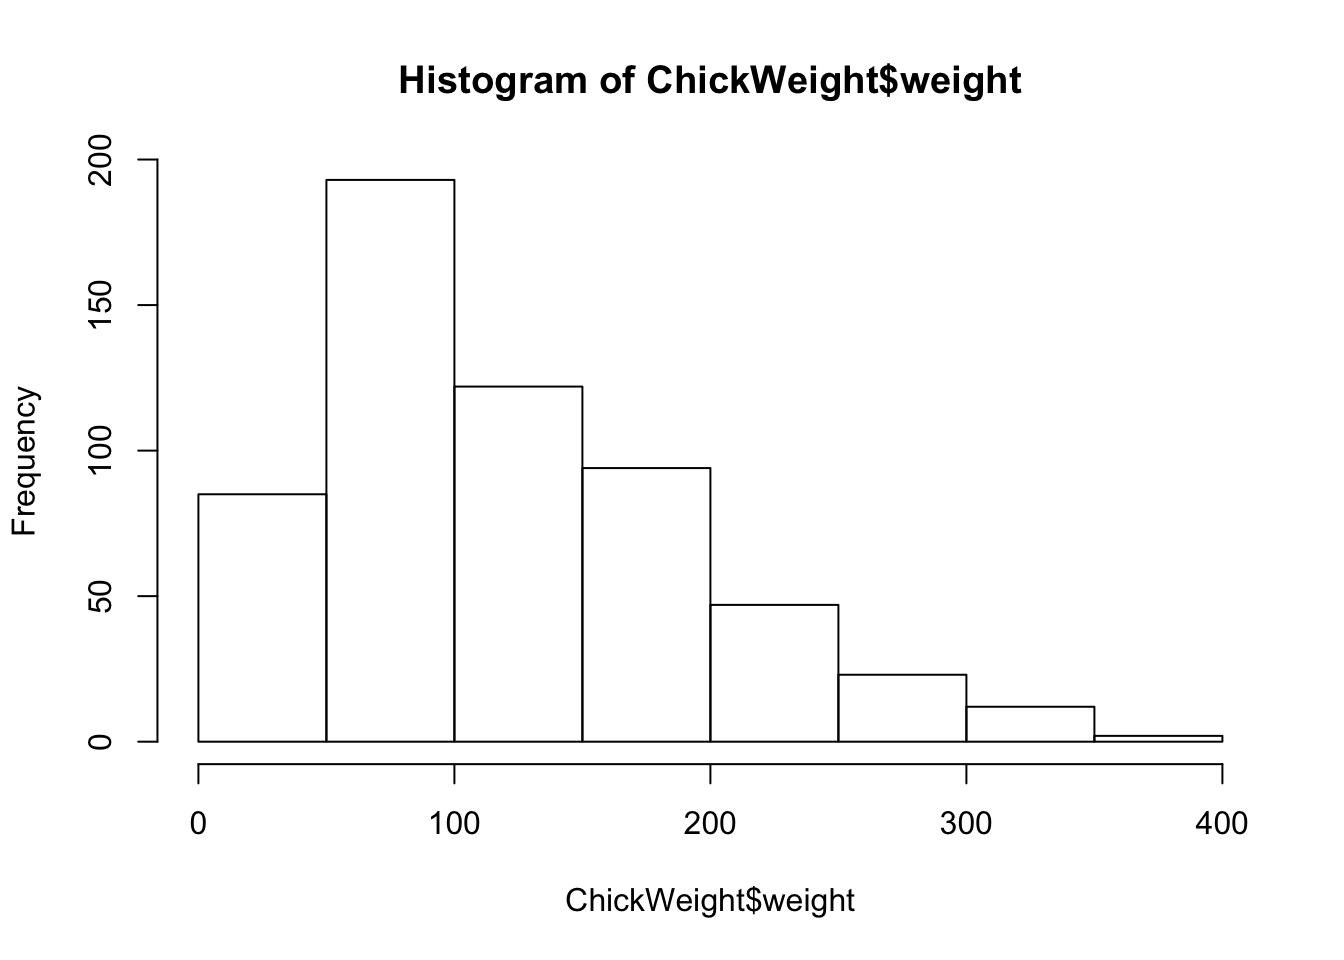
\includegraphics{Data-Analysis-for-Psychology_files/figure-latex/plot_chap03-2.pdf}

\begin{Shaded}
\begin{Highlighting}[]
\KeywordTok{boxplot}\NormalTok{(InsectSprays}\OperatorTok{$}\NormalTok{count}\OperatorTok{~}\NormalTok{InsectSprays}\OperatorTok{$}\NormalTok{spray)}
\end{Highlighting}
\end{Shaded}

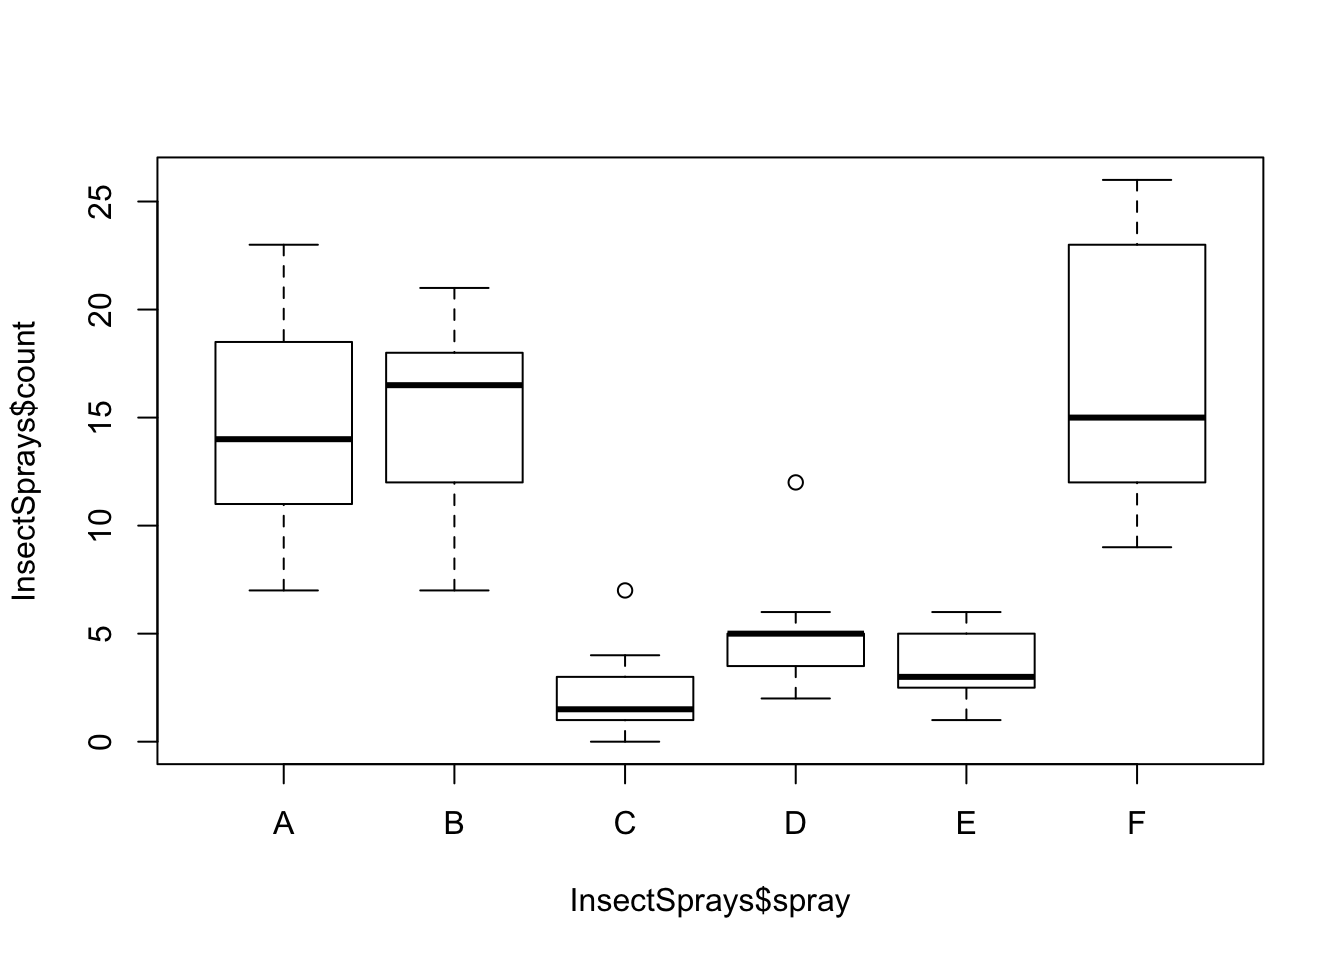
\includegraphics{Data-Analysis-for-Psychology_files/figure-latex/plot_chap03-3.pdf}

今後もわからないことが出てきたら,関数のヘルプを参照すること(英語だが)。あるいはインターネットで検索する。

\begin{Shaded}
\begin{Highlighting}[]
\CommentTok{#関数の前に?を入れて実行すると,ヘルプが表示される。あるいはhelp()で囲む}
\NormalTok{?qplot}
\KeywordTok{help}\NormalTok{(qplot)}
\end{Highlighting}
\end{Shaded}

\subsection{練習問題}\label{-3}

\subsubsection{問1}\label{-6}

Rにサンプルデータとして入っているChickWeightを使ってグラフを作ってみよう。

\begin{Shaded}
\begin{Highlighting}[]
\KeywordTok{head}\NormalTok{(ChickWeight)}
\end{Highlighting}
\end{Shaded}

\begin{verbatim}
## Grouped Data: weight ~ Time | Chick
##   weight Time Chick Diet
## 1     42    0     1    1
## 2     51    2     1    1
## 3     59    4     1    1
## 4     64    6     1    1
## 5     76    8     1    1
## 6     93   10     1    1
\end{verbatim}

\begin{itemize}
\tightlist
\item
  ChickWeightには,ひよこを対象とした実験データが入っている。食事を変えると体重が変化するかどうかを調べた。まず,ChickWeightと入力して,データの中身を確認する。
\item
  日数(Time)と体重(weight)の間の関係を散布図で確認する。
\item
  体重(weight)の分布をヒストグラムで確認する。
\item
  食事の種類(Diet)ごとに体重(weight)の分布を箱ひげ図を作って確認する。
\end{itemize}

\subsubsection{問2}\label{-7}

ある学校の生徒を対象に行った調査の結果,YouTubeの視聴時間と学校での成績の間の相関係数を測ったところ,r
= -
.56であった。この調査の結果から,「YouTubeを見るほど,学力が下がる」という結論を出せるか?別の解釈が可能だと思うのならば,その解釈を述べよ。また,「YouTubeを見るほど,学力が下がる」ということを調べるためにはどうすれば良いと思うかを述べよ。

\subsection{参考文献}

中室牧子・津川友介 (2017).
「原因と結果」の経済学ーデータから真実を見抜く思考 ダイヤモンド社

\section{確率分布}

\begin{itemize}
\tightlist
\item
  確率分布とは何かについて学ぶ。

  \begin{itemize}
  \tightlist
  \item
    確率変数と確率分布
  \item
    二項分布
  \item
    正規分布
  \item
    その他の確率分布
  \end{itemize}
\end{itemize}

\subsection{はじめに}\label{-1}

今回の演習でも,tidyverseパッケージを使うので,予めロードしておく。また,set.seed(1234)というプログラムを実行しておく。

\begin{itemize}
\tightlist
\item
  set.seed()はいわゆる「乱数の種」というものを設定するための関数。乱数の種を同じ値に設定しておくと,乱数を再現することが出来る(このテキストに書いてあるのと同じ結果が再現できる)。
\end{itemize}

\begin{Shaded}
\begin{Highlighting}[]
\KeywordTok{install.packages}\NormalTok{(}\StringTok{"tidyverse"}\NormalTok{)}
\KeywordTok{library}\NormalTok{(tidyverse)}
\KeywordTok{set.seed}\NormalTok{(}\DecValTok{1234}\NormalTok{)}
\end{Highlighting}
\end{Shaded}

\subsection{確率変数と確率分布}

サイコロを1個投げるとする。それぞれの目が出る確率は1/6である。それぞれの目をX(1,
2, 3, 4, 5, 6),それぞれの目が出る確率をP(X)とする。\\
XとP(X)を以下の表1で示す。

表1\\
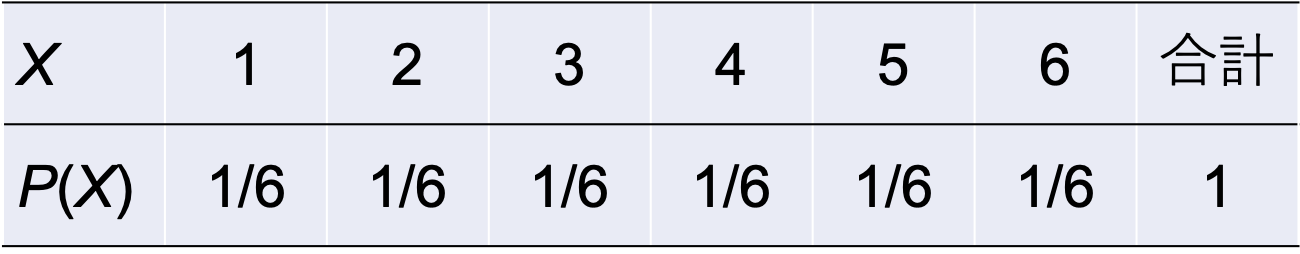
\includegraphics{04_table01.png}

このとき,Xを\textbf{確率変数}と呼ぶ。その値と対応する確率が存在する変数のことをいう。表1のように,確率変数とその変数が取り得る確率の分布を\textbf{確率分布}という。

確率分布には様々な種類がある。今回は特に,その中でも\textbf{二項分布}と\textbf{正規分布}について扱う。

※なお,上のサイコロの目の例のように,どの確率変数Xについても常に一定値の確率を取る確率分布は\textbf{一様分布(uniform
distribution)}と呼ばれる。

\subsection{二項分布}

\subsubsection{二項分布の基本}

コインをn回投げる。表が出る確率を\(q\)とすると,
裏が出る確率は\((1-q)\)となる。n回中,表がx回出る確率P(x)は,理論的には以下の式で算出される。

\[
P(x) = {}_n\mathrm{C}_xq^{x}(1-q)^{(n-x)}
\]

xを確率変数とした場合,上記の式の確率に従う確率分布を\textbf{二項分布}という。
つまり二項分布は,\textbf{生じる事象が2つのカテゴリに分けられる場合}に当てはまる確率分布である。コインを投げたときに出る面が「表か裏」か,学生の中から選んだ人の性別が「男か女」か,ある意見について「賛成か反対」かなど。このような事象が生じる確率は,理論的には二項分布に従う。

コインを投げる場合の例に戻る。例えば,表が出る確率qを0.5として,10回投げたときに表が6回出る確率を計算してみよう。Rならば,dbinom()関数を使えば簡単に計算できる。

\begin{Shaded}
\begin{Highlighting}[]
\CommentTok{#xは確率変数(コインの例での),sizeは試行回数(コインの例のnに相当),}
\KeywordTok{dbinom}\NormalTok{(}\DataTypeTok{x=}\DecValTok{6}\NormalTok{, }\DataTypeTok{size=}\DecValTok{10}\NormalTok{, }\DataTypeTok{prob=}\FloatTok{0.5}\NormalTok{)}
\end{Highlighting}
\end{Shaded}

\begin{verbatim}
## [1] 0.2050781
\end{verbatim}

\begin{Shaded}
\begin{Highlighting}[]
\CommentTok{#上の式n, x, pに実際に値を入れて計算する場合。dbinom()関数を使った場合と結果が一致することを確認しよう。}
\KeywordTok{choose}\NormalTok{(}\DecValTok{10}\NormalTok{, }\DecValTok{6}\NormalTok{) }\OperatorTok{*}\StringTok{ }\FloatTok{0.5}\OperatorTok{^}\DecValTok{6} \OperatorTok{*}\StringTok{ }\NormalTok{(}\DecValTok{1} \OperatorTok{-}\StringTok{ }\FloatTok{0.5}\NormalTok{) }\OperatorTok{^}\DecValTok{4}
\end{Highlighting}
\end{Shaded}

\begin{verbatim}
## [1] 0.2050781
\end{verbatim}

二項分布は以下のように表現されることもある。

\[
x \sim Binomial(n, q)
\]

Binomialのカッコ内のn,
qのように,確率分布を構成する変数のことをパラメータと呼ぶ。
Binomialは二項分布,\(\sim\)は「従う」という意味である。つまりこの式は,「xは,nとqをパラメータとする二項分布に従う」ということをいっている。

\subsubsection{二項分布の期待値と分散}

表が出る回数xが0〜10回の場合全てについて,それぞれが生じる確率を計算すると以下のようになる。

\begin{Shaded}
\begin{Highlighting}[]
\KeywordTok{dbinom}\NormalTok{(}\DataTypeTok{x=}\DecValTok{0}\OperatorTok{:}\DecValTok{10}\NormalTok{, }\DataTypeTok{size=}\DecValTok{10}\NormalTok{, }\DataTypeTok{prob=}\FloatTok{0.5}\NormalTok{)}
\end{Highlighting}
\end{Shaded}

\begin{verbatim}
##  [1] 0.0009765625 0.0097656250 0.0439453125 0.1171875000 0.2050781250
##  [6] 0.2460937500 0.2050781250 0.1171875000 0.0439453125 0.0097656250
## [11] 0.0009765625
\end{verbatim}

グラフにすると以下のようになる。横軸をx, 縦軸をP(x)とする。

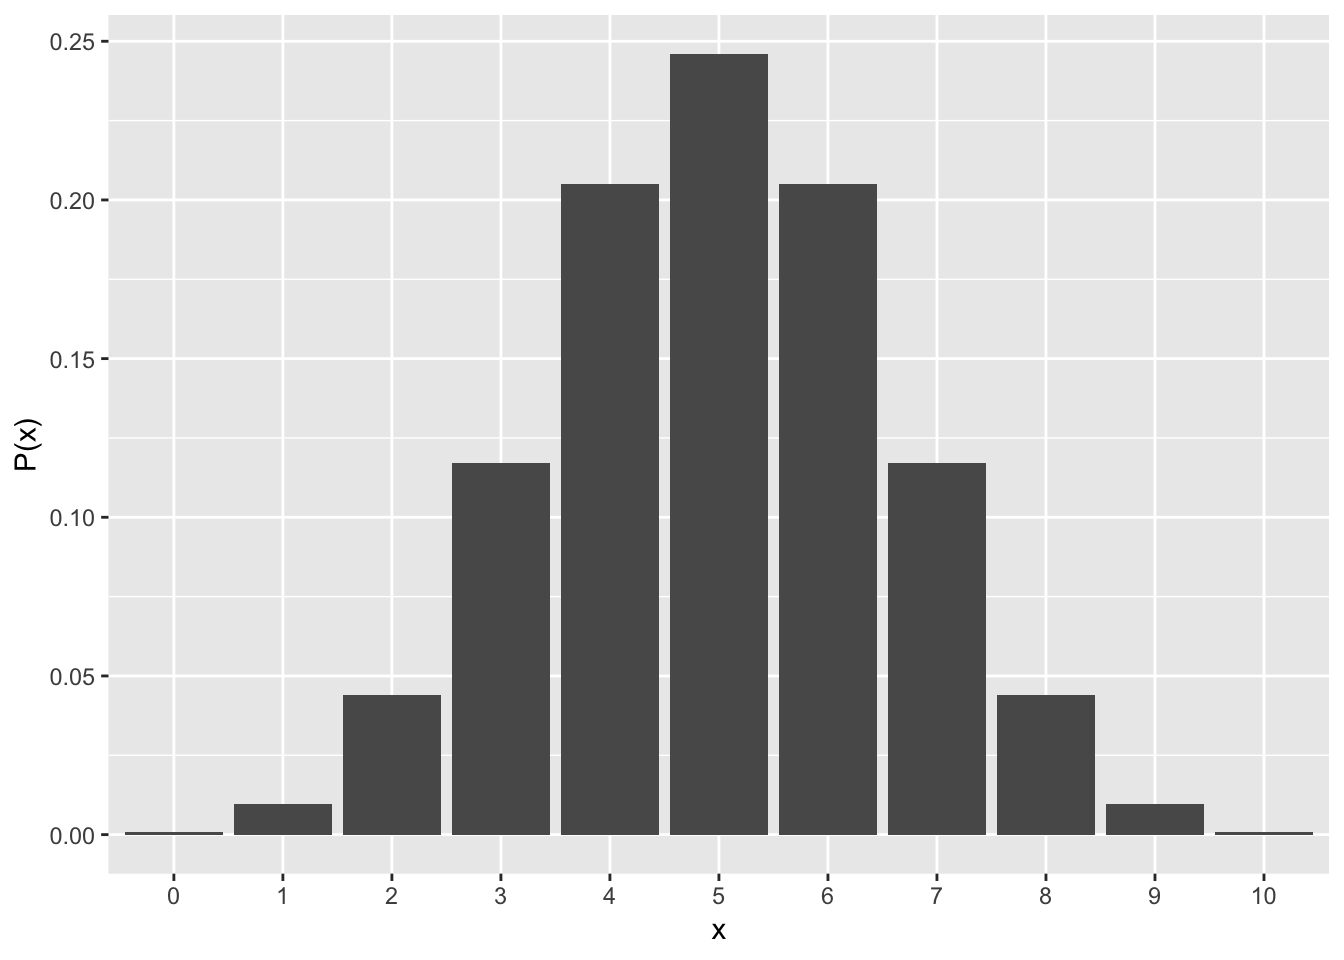
\includegraphics{Data-Analysis-for-Psychology_files/figure-latex/dbinom_2_plot_chap04-1.pdf}

グラフからもわかるように,表が出る確率が0.5のコインを10回投げたときに,最も出やすいのは10回中5回であることがわかる。10回中1回,10回中10回出るケースはほとんどまれであることがわかる。\\
この図からも,確率分布には最も出やすい変数(平均値。確率分布の場合は期待値と呼ぶ)と分散が存在することがわかる。

二項分布の期待値\(E(x)\)と分散\(Var(x)\)は,以下の式から計算できる。

\[
E(x) = nq\\
Var(x) = nq(1-q)
\]

表が出る確率が0.5(i.e., q=0.5)のコインを10回(i.e.,
n=10)投げた場合における,表が出る回数xの期待値と分散を計算してみよう。

\begin{Shaded}
\begin{Highlighting}[]
\CommentTok{#E(x) = nq}
\DecValTok{10}\OperatorTok{*}\FloatTok{0.5}
\end{Highlighting}
\end{Shaded}

\begin{verbatim}
## [1] 5
\end{verbatim}

\begin{Shaded}
\begin{Highlighting}[]
\CommentTok{#Var(x) = nq(1-q)}
\DecValTok{10}\OperatorTok{*}\FloatTok{0.5}\OperatorTok{*}\NormalTok{(}\DecValTok{1}\OperatorTok{-}\FloatTok{0.5}\NormalTok{)}
\end{Highlighting}
\end{Shaded}

\begin{verbatim}
## [1] 2.5
\end{verbatim}

n=1のときは,\emph{ベルヌーイ分布}と呼ばれる(例えばコインを1回だけ投げる場合)。

\subsection{正規分布}

\subsubsection{正規分布の基礎}

統計学で用いられる確率分布の中でも有名なのは\emph{正規分布}である。正規分布は,平均\(\mu\),標準偏差\(\sigma\)をパラメータとする確率分布で,釣鐘型(ベル・カーブ)状の分布を描く。

平均\(\mu\),標準偏差\(\sigma\)とする正規分布の確率密度関数f(x)は,以下の式から計算される。

\begin{itemize}
\item
  この式自体を覚える必要はない。
\item
  これは確率分布ではなく,\emph{確率密度関数}と呼ばれるものである。確率分布は縦軸が横軸の値それぞれが生じる確率を意味しているが,確率密度関数の縦軸は確率そのものを意味しない。確率密度関数の面積が確率を意味する。すなわち,確率密度関数の面積全てを合計した値は,1となる。
\end{itemize}

\[
f(x) = \frac{1}{\sqrt{2\pi\sigma^2}}\exp\left(-\frac{(x-\mu)^2}{2\sigma^2}\right)
\] または,以下のように表現することもある。

\[
x \sim Normal(\mu, \sigma)
\]

平均\(\mu\)を0,標準偏差\(\sigma\)を1とする正規分布について考えてみる。\\
Rならば,dnorm関数で確率密度関数を出力することができる。

\begin{Shaded}
\begin{Highlighting}[]
\NormalTok{x =}\StringTok{ }\KeywordTok{seq}\NormalTok{(}\OperatorTok{-}\DecValTok{3}\NormalTok{, }\DecValTok{3}\NormalTok{, }\FloatTok{0.05}\NormalTok{)}
\NormalTok{y =}\StringTok{ }\KeywordTok{dnorm}\NormalTok{(}\DataTypeTok{x=}\NormalTok{x, }\DataTypeTok{mean=}\DecValTok{0}\NormalTok{, }\DataTypeTok{sd=}\DecValTok{1}\NormalTok{)}
\NormalTok{y}
\end{Highlighting}
\end{Shaded}

これをグラフにすると以下のようになる。

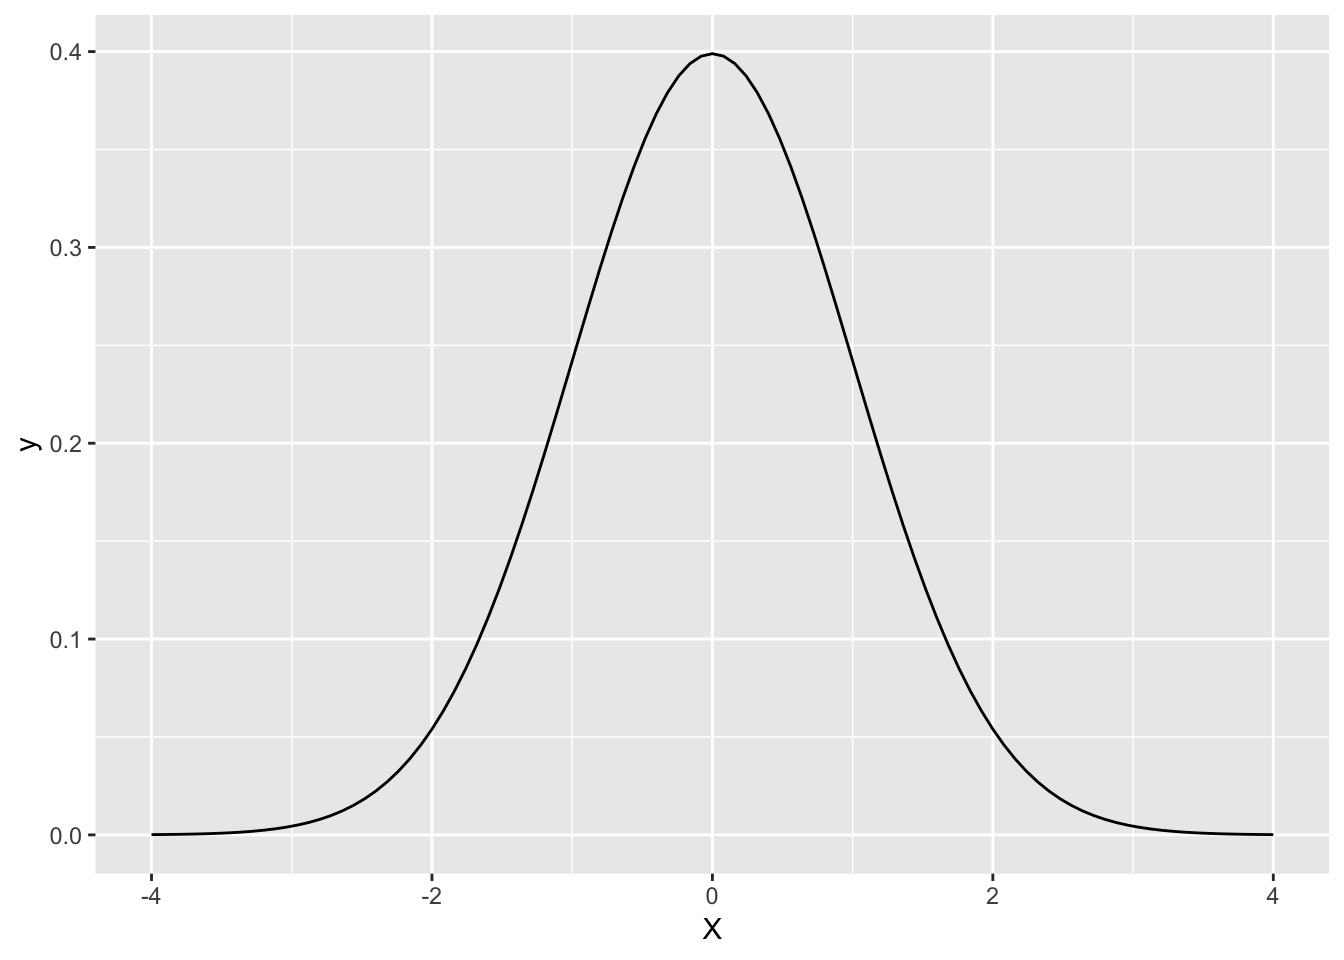
\includegraphics{Data-Analysis-for-Psychology_files/figure-latex/norm_distribution_plot_chap04-1.pdf}

x=0からx=1の範囲が生じる確率は,その範囲に対応するグラフの面積となる。

\begin{Shaded}
\begin{Highlighting}[]
\CommentTok{#Rならば,pnorm関数でxが-∞からqまでの範囲の確率を求めることができる}
\CommentTok{#以下は,平均0,標準偏差1の正規分布で 0までの確率を求めている。正規分布の半分に相当するので,0.5である。}
\KeywordTok{pnorm}\NormalTok{(}\DataTypeTok{q=}\DecValTok{0}\NormalTok{, }\DataTypeTok{mean=}\DecValTok{0}\NormalTok{, }\DataTypeTok{sd=}\DecValTok{1}\NormalTok{)}
\end{Highlighting}
\end{Shaded}

\begin{verbatim}
## [1] 0.5
\end{verbatim}

\begin{Shaded}
\begin{Highlighting}[]
\CommentTok{#特定の範囲を求めたい場合は以下のように使えば良い。例えば以下は,xが1から2の範囲の確率である。}
\NormalTok{x =}\StringTok{ }\KeywordTok{pnorm}\NormalTok{(}\DataTypeTok{q=}\DecValTok{2}\NormalTok{, }\DataTypeTok{mean=}\DecValTok{0}\NormalTok{, }\DataTypeTok{sd=}\DecValTok{1}\NormalTok{) }\OperatorTok{-}\StringTok{ }\KeywordTok{pnorm}\NormalTok{(}\DataTypeTok{q=}\DecValTok{1}\NormalTok{, }\DataTypeTok{mean=}\DecValTok{0}\NormalTok{, }\DataTypeTok{sd=}\DecValTok{1}\NormalTok{) }
\NormalTok{x}
\end{Highlighting}
\end{Shaded}

\begin{verbatim}
## [1] 0.1359051
\end{verbatim}

以下が平均\(\mu\)と標準偏差\(\sigma\)の値をそれぞれ変えた場合の正規分布である。

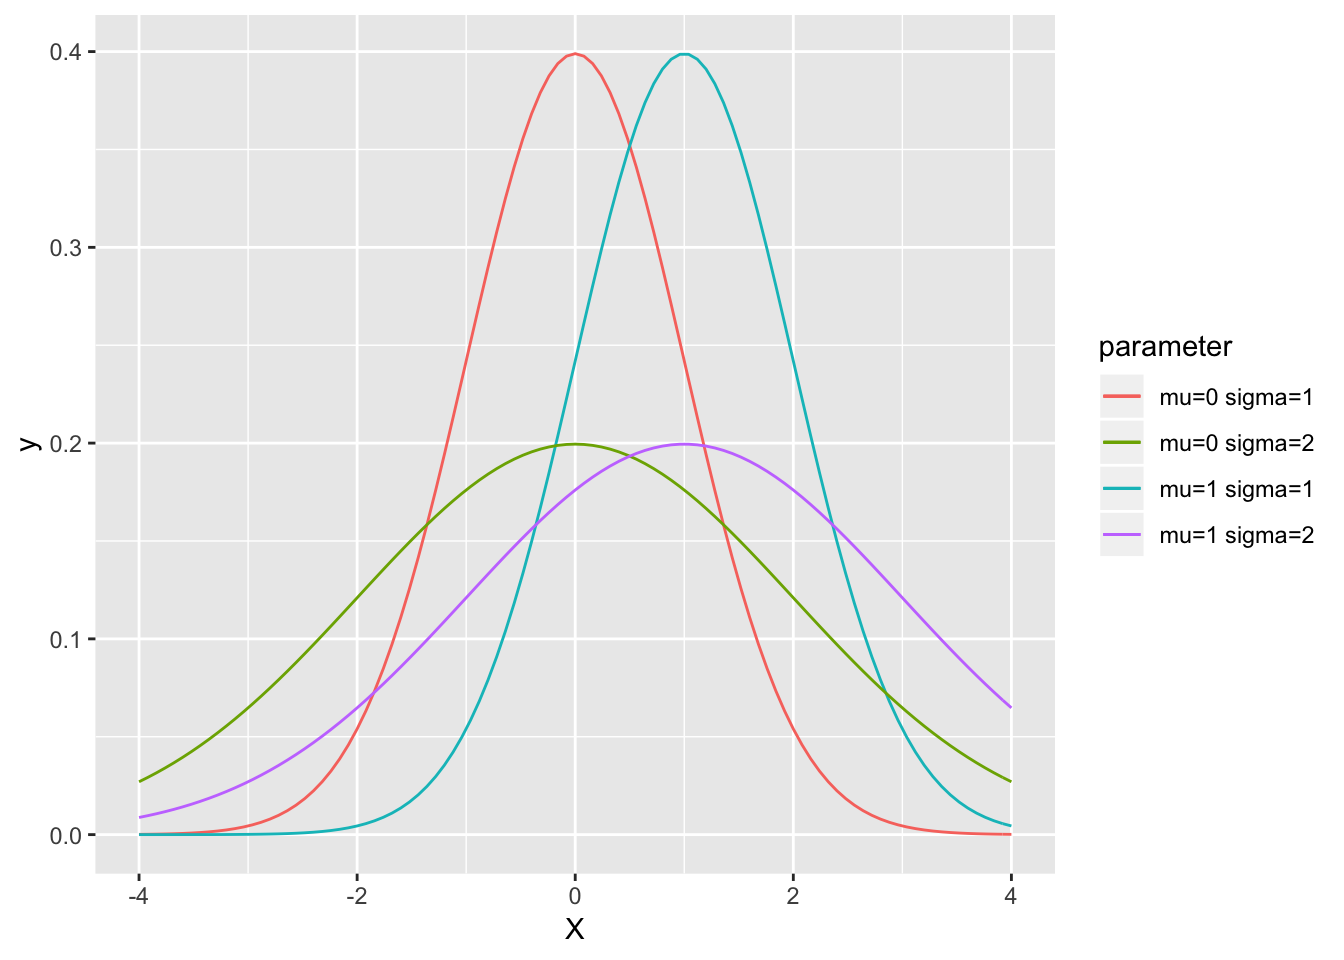
\includegraphics{Data-Analysis-for-Psychology_files/figure-latex/norm_distribution_plot2_chap04-1.pdf}

\begin{itemize}
\item
  正規分布は平均\(\mu\)を対象として左右対称のかたちを描く。
\item
  統計学では様々な変数について,「変数が正規分布に従う」という仮定を置くことが多い。体重や身長なども経験的に正規分布を描く。正規分布は以降でも述べるように確率変数xが連続量の場合の確率分布であるが,離散値のデータについても正規分布を仮定して分析することもよくある(テストの点数,質問紙の回答得点など)。
\item
  しかし,世の中には正規分布に従わない変数もある(例えば年収などは釣鐘型の分布にならない)。データ分析の前に事前に実際のデータの分布を見て,左右対称でないなど明らかに正規分布を仮定できない変数については分析のやりかたを考える必要がある。
\item
  平均0, 標準偏差1の正規分布は\textbf{標準正規分布}と呼ばれる。
\item
  二項分布\(Binomial(n, p)\)の\(n\)が十分に大きい場合,二項分布は正規分布\(Normal(np, \sqrt{np(1-p)})\)に近似する。例えば,以下にn=50のときの二項分布を示す。
\end{itemize}

\begin{Shaded}
\begin{Highlighting}[]
\CommentTok{#n=50のとき}
\NormalTok{plot <-}\StringTok{ }\KeywordTok{data.frame}\NormalTok{(}\DataTypeTok{x=}\DecValTok{0}\OperatorTok{:}\DecValTok{50}\NormalTok{, }\DataTypeTok{p=}\KeywordTok{dbinom}\NormalTok{(}\DataTypeTok{x=}\DecValTok{0}\OperatorTok{:}\DecValTok{50}\NormalTok{, }\DataTypeTok{size=}\DecValTok{50}\NormalTok{, }\DataTypeTok{prob=}\FloatTok{0.5}\NormalTok{))}
\NormalTok{p <-}\StringTok{ }\KeywordTok{ggplot}\NormalTok{(}\DataTypeTok{data=}\NormalTok{plot, }\KeywordTok{aes}\NormalTok{(}\DataTypeTok{x=}\KeywordTok{factor}\NormalTok{(x), }\DataTypeTok{y=}\NormalTok{p)) }\OperatorTok{+}\StringTok{ }\KeywordTok{geom_bar}\NormalTok{(}\DataTypeTok{stat=}\StringTok{"identity"}\NormalTok{) }\OperatorTok{+}\StringTok{ }\KeywordTok{ylab}\NormalTok{(}\StringTok{"P(x)"}\NormalTok{) }\OperatorTok{+}\StringTok{ }\KeywordTok{xlab}\NormalTok{(}\StringTok{"x"}\NormalTok{)}
\NormalTok{p}
\end{Highlighting}
\end{Shaded}

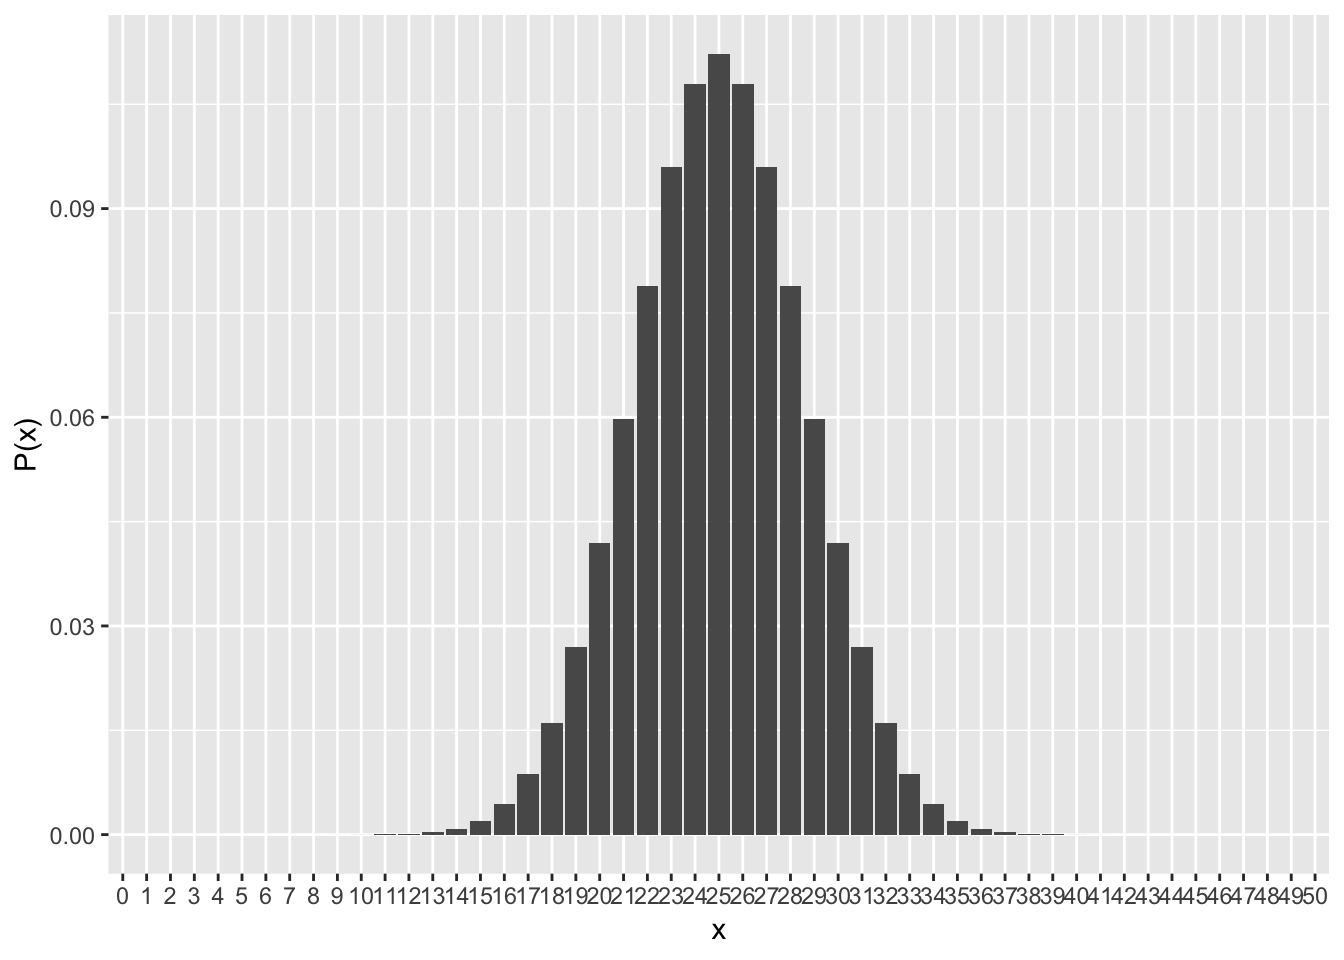
\includegraphics{Data-Analysis-for-Psychology_files/figure-latex/binom_norm_chap04-1.pdf}

\subsubsection{中心極限定理}

\begin{itemize}
\tightlist
\item
  「母集団の確率分布が平均\(\mu\),標準偏差\(\sigma\)を持つ確率分布に従う\(X\)について,その平均値\(\bar{X_{n}}\)はnが大きくなれば,平均\(\mu\),標準偏差\(\sigma\)の正規分布に収束する」というのが中心極限定理である。
\item
  元の分布がどのような分布でも,そこから平均値を計算することを何回も繰り返すとその分布は正規分布のかたちになるということ。\\
\item
  シミュレーションで確認する。6面のサイコロを100回振る実験を行うとする。
\end{itemize}

\begin{Shaded}
\begin{Highlighting}[]
\NormalTok{X <-}\StringTok{ }\KeywordTok{round}\NormalTok{(}\KeywordTok{runif}\NormalTok{(}\DecValTok{100}\NormalTok{,}\DataTypeTok{min=}\DecValTok{1}\NormalTok{,}\DataTypeTok{max=}\DecValTok{6}\NormalTok{),}\DecValTok{0}\NormalTok{)}
\KeywordTok{mean}\NormalTok{(X)}
\end{Highlighting}
\end{Shaded}

\begin{verbatim}
## [1] 3.24
\end{verbatim}

\begin{itemize}
\item
  それぞれの目が出る確率は1/6で一定である。すなわち,サイコロが出る目は一様分布に従う(正規分布ではない)。\\
\item
  一様分布の平均値は,最大値をa,
  最小値をbとすると,(a+b)/2。すなわち,サイコロの例の場合の平均値は理論的には(1+6)/2=3.5となる。
\item
  サイコロを100回振って平均値を求める。この平均値を求めるのを,1,000回繰り返し行う。求めた平均値1,000個の分布を見てみると。。
\end{itemize}

\begin{Shaded}
\begin{Highlighting}[]
\NormalTok{sample.means <-}\StringTok{ }\KeywordTok{sapply}\NormalTok{(}\KeywordTok{c}\NormalTok{(}\DecValTok{1}\OperatorTok{:}\DecValTok{1000}\NormalTok{), }\ControlFlowTok{function}\NormalTok{(x) \{}\KeywordTok{mean}\NormalTok{(}\KeywordTok{round}\NormalTok{(}\KeywordTok{runif}\NormalTok{(}\DecValTok{100}\NormalTok{,}\DataTypeTok{min=}\DecValTok{1}\NormalTok{,}\DataTypeTok{max=}\DecValTok{6}\NormalTok{),}\DecValTok{0}\NormalTok{))\} )}
\KeywordTok{qplot}\NormalTok{(sample.means)}
\end{Highlighting}
\end{Shaded}

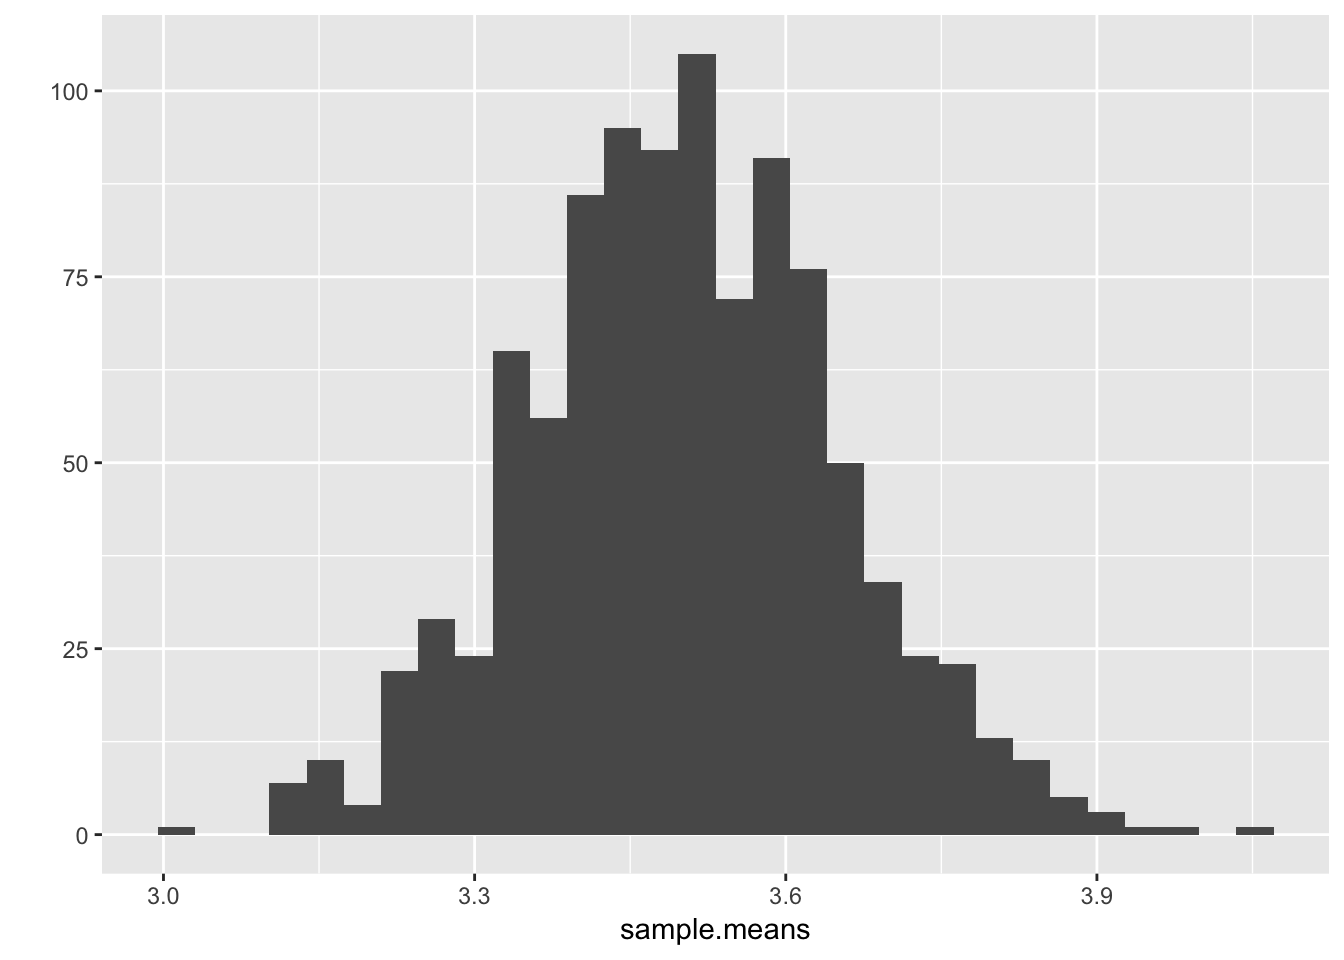
\includegraphics{Data-Analysis-for-Psychology_files/figure-latex/central_limit_1000_chap04-1.pdf}

\begin{itemize}
\item
  正規分布に近似する。1,000回よりももっと回数を増やすと,より正規分布っぽいかたちになる。
\item
  このように,元の母集団の分布がたとえ正規分布でなくても,その標本平均は正規分布に近似する。
\end{itemize}

\begin{Shaded}
\begin{Highlighting}[]
\CommentTok{#サイコロを7回振ってその合計を求める。これを10,000回行ったときの出目の合計値の分布}
\NormalTok{Y <-}\StringTok{ }\KeywordTok{round}\NormalTok{(}\KeywordTok{runif}\NormalTok{(}\DecValTok{10000}\NormalTok{,}\DataTypeTok{min=}\DecValTok{1}\NormalTok{,}\DataTypeTok{max=}\DecValTok{6}\NormalTok{),}\DecValTok{0}\NormalTok{) }\OperatorTok{+}\KeywordTok{round}\NormalTok{(}\KeywordTok{runif}\NormalTok{(}\DecValTok{10000}\NormalTok{,}\DataTypeTok{min=}\DecValTok{1}\NormalTok{,}\DataTypeTok{max=}\DecValTok{6}\NormalTok{),}\DecValTok{0}\NormalTok{) }\OperatorTok{+}\KeywordTok{round}\NormalTok{(}\KeywordTok{runif}\NormalTok{(}\DecValTok{10000}\NormalTok{,}\DataTypeTok{min=}\DecValTok{1}\NormalTok{,}\DataTypeTok{max=}\DecValTok{6}\NormalTok{),}\DecValTok{0}\NormalTok{) }\OperatorTok{+}\KeywordTok{round}\NormalTok{(}\KeywordTok{runif}\NormalTok{(}\DecValTok{10000}\NormalTok{,}\DataTypeTok{min=}\DecValTok{1}\NormalTok{,}\DataTypeTok{max=}\DecValTok{6}\NormalTok{),}\DecValTok{0}\NormalTok{) }\OperatorTok{+}\KeywordTok{round}\NormalTok{(}\KeywordTok{runif}\NormalTok{(}\DecValTok{10000}\NormalTok{,}\DataTypeTok{min=}\DecValTok{1}\NormalTok{,}\DataTypeTok{max=}\DecValTok{6}\NormalTok{),}\DecValTok{0}\NormalTok{) }\OperatorTok{+}\KeywordTok{round}\NormalTok{(}\KeywordTok{runif}\NormalTok{(}\DecValTok{10000}\NormalTok{,}\DataTypeTok{min=}\DecValTok{1}\NormalTok{,}\DataTypeTok{max=}\DecValTok{6}\NormalTok{),}\DecValTok{0}\NormalTok{) }\OperatorTok{+}\KeywordTok{round}\NormalTok{(}\KeywordTok{runif}\NormalTok{(}\DecValTok{10000}\NormalTok{,}\DataTypeTok{min=}\DecValTok{1}\NormalTok{,}\DataTypeTok{max=}\DecValTok{6}\NormalTok{),}\DecValTok{0}\NormalTok{)}
\KeywordTok{qplot}\NormalTok{(Y)}
\end{Highlighting}
\end{Shaded}

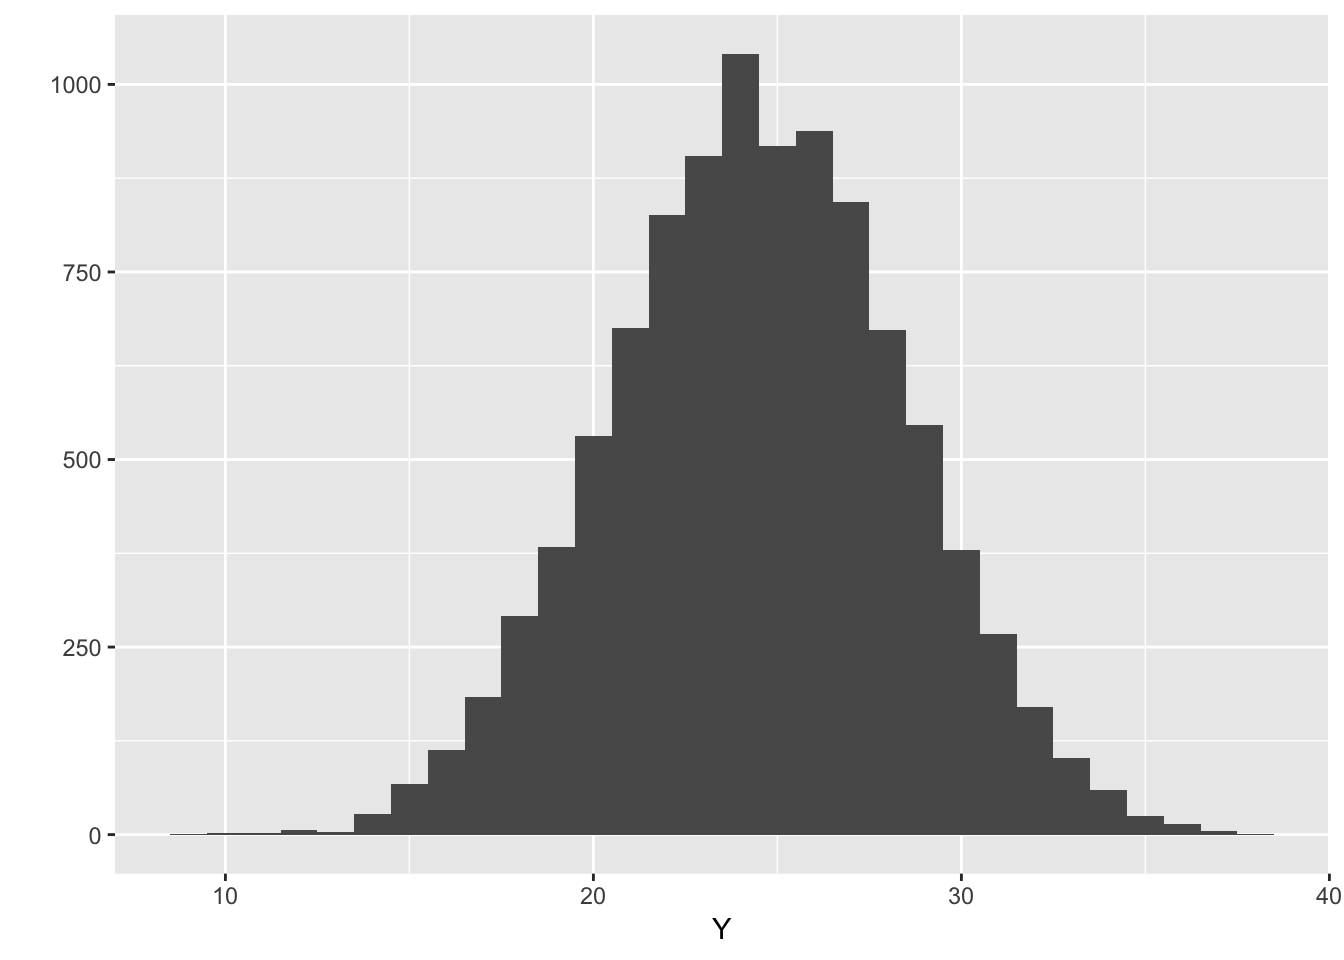
\includegraphics{Data-Analysis-for-Psychology_files/figure-latex/central_limit_2_chap04-1.pdf}

\begin{itemize}
\tightlist
\item
  中心極限定理が成り立つため,たとえ元の変数が正規分布に従ってなくても,平均化したものを使えば正規分布を前提とした統計的仮説検定を行なっても大きな問題はない。

  \begin{itemize}
  \tightlist
  \item
    複数の質問項目(順序尺度)をまとめて平均化した心理尺度を分析に使う。
  \item
    選挙への投票(「した」もしくは「しなかった」の二値)者の割合を県ごとに算出して,県を単位として分析に使う。
  \end{itemize}
\end{itemize}

\subsection{その他の確率分布}

二項分布のように,確率変数xが離散変数の場合の確率分布は,\textbf{離散確率分布}という。\\
正規分布のように,確率変数xが連続変数の場合は,\textbf{連続確率分布}という。

他にも確率分布は以下のようなものがある。

\subsubsection{離散確率分布}

\paragraph{ポアソン分布}

\[
P(x) = \frac{\lambda^x\exp(-\lambda)}{x!}\\
x \sim Poisson(\lambda)\\
\]

\begin{itemize}
\tightlist
\item
  xは0以上の整数(0, 1, 2, 3, \ldots{})とする。\\
\item
  ポアソン分布のパラメータは\(\lambda\)だけである。期待値(平均)は\(\lambda\),分散は\(\lambda\)である。つまり,平均と分散が等しい分布である。
\item
  以下に,パラメータ\(\lambda\)をそれぞれ変えた場合のポアソン分布を示す。
\end{itemize}

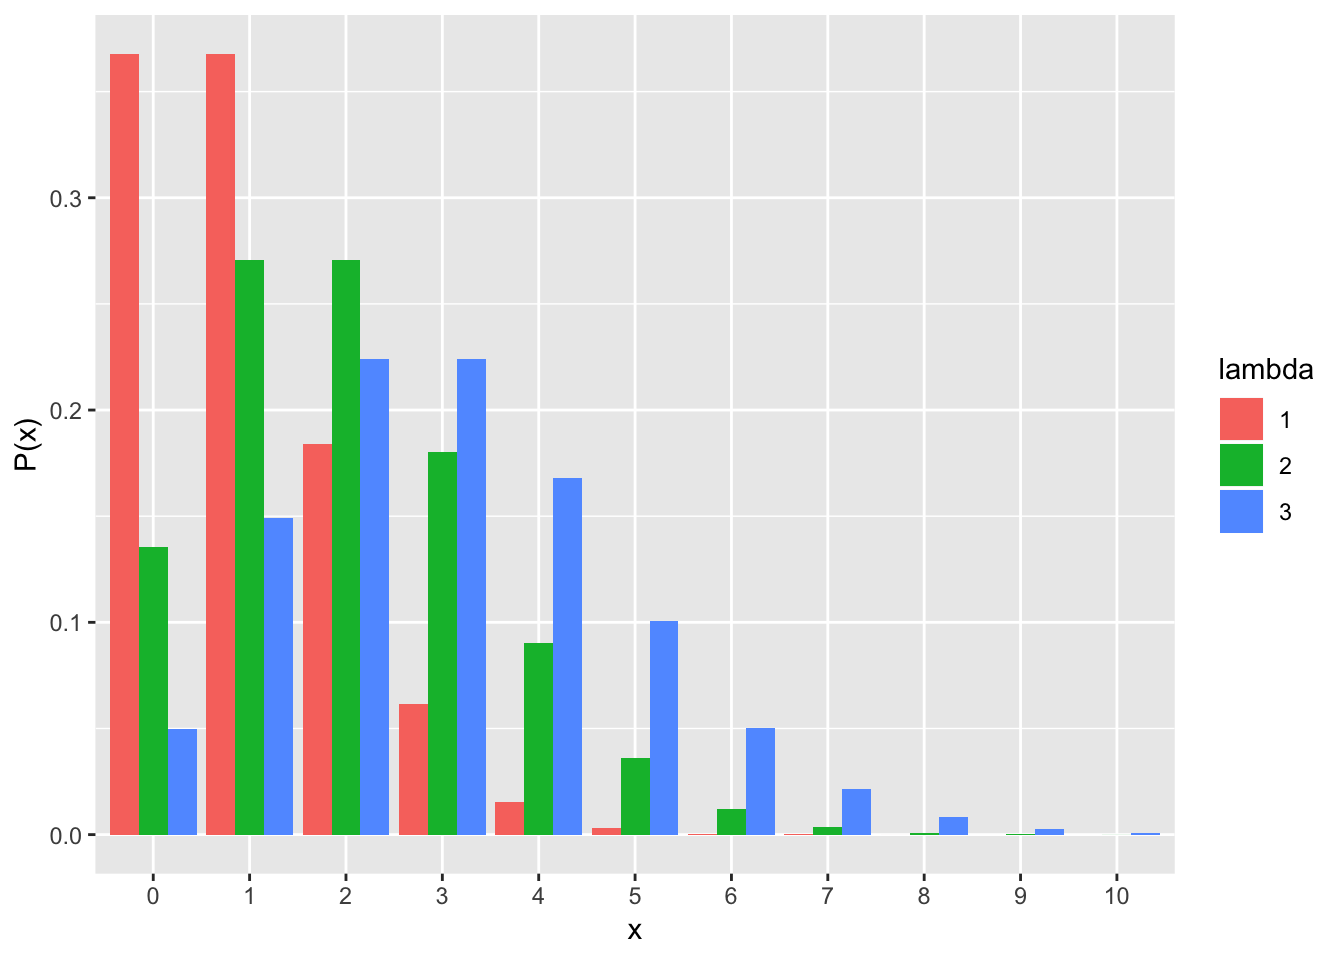
\includegraphics{Data-Analysis-for-Psychology_files/figure-latex/poisson_distribution_plot2_chap04-1.pdf}

\begin{itemize}
\item
  一定の期間中にランダムで生じる事象はポアソン分布に従う。具体的な例としては,1日の間に届くメールの件数,営業時間中に来る客の数など。
\item
  二項分布\(Binomial(n, p)\)の\(n\)が十分大きく,かつ\(p\)が小さい場合は平均を\(np\)とするポアソン分布に近似する。つまり,めったに起こらない事象はポアソン分布に従う。例えば,1年間の間に生じる交通事故の件数など(365日それぞれで0.1\%で生じるとした場合)。歴史的に有名な例は,「ドイツ軍で1年間で馬に蹴られて死亡した兵士の数」がポアソン分布に従うというもの。
\end{itemize}

\subsubsection{連続確率分布}

\paragraph{t分布}\label{t}

\[
P(x) = \frac{\Gamma((v+1)/2)}{\Gamma(v/2)\sqrt{\pi v}\sigma}\left(1+\frac{1}{v}\left(\frac{x-\mu}{\sigma}\right)^2\right)^{-(v+1)/2}\\
x \sim Student\_t(v, \mu, \sigma)\\
\]

\begin{itemize}
\tightlist
\item
  パラメータは3つ。vは自由度と呼ばれる。\\
\item
  自由度の小さいt分布は分布の裾が長くなる。すなわち,外れ値を含んだ分布となる。
\item
  自由度\(\infty\)のt分布は正規分布と一致する。
\end{itemize}

連続確率分布には他にも対数正規分布,指数分布などがあるが,とりあえずは正規分布を知っておけば良い。

\subsection{練習問題}\label{-4}

\subsubsection{問1}\label{-8}

\begin{itemize}
\item
  あなたは野球部の監督で,自分のチームの勝率はこれまでの練習の経験から32\%だとわかっている。
\item
  これから遠征で,全部で10試合を行う予定である。
\item
  勝つ試合の回数を確率変数nとし,nとそれぞれのnに対応する確率を表で示せ。
\item
  平均して何試合勝つことができるかを述べよ。
\end{itemize}

\subsubsection{問2}\label{-9}

\begin{itemize}
\item
  ある学校で小学6年生の身長を測ったところ,平均は150.2 cmで標準偏差が3.5
  cmであった。
\item
  身長152 cmから155 cmの児童の割合はいくらか。
\item
  身長158 cmを超える児童は何割いるか。

  \begin{itemize}
  \tightlist
  \item
    ヒント:pnorm関数を使おう。なお,全ての範囲の確率の合計は1である。
  \end{itemize}
\end{itemize}

\section{統計的帰無仮説検定}

\begin{itemize}
\tightlist
\item
  統計的帰無仮説検定の考え方について理解する。

  \begin{itemize}
  \tightlist
  \item
    統計的帰無仮説検定の考え方(p値とは何か?)
  \item
    第1種の過誤と第2種の過誤
  \item
    多重検定
  \end{itemize}
\end{itemize}

\subsection{準備}\label{-2}

今回もtidyverseパッケージを使う。予めインストールの上,ロードをしておく。

\begin{Shaded}
\begin{Highlighting}[]
\KeywordTok{install.packages}\NormalTok{(}\StringTok{"tidyverse"}\NormalTok{)}
\KeywordTok{library}\NormalTok{(tidyverse)}
\end{Highlighting}
\end{Shaded}

\subsection{統計的帰無仮説検定の考え方}

以降では,前回学んだ二項分布を用いた統計的帰無仮説検定(二項検定)を例としながら,統計的帰無仮説検定の考え方について理解していく。

\subsubsection{二項分布の復習}

コインを10回投げて表が出た回数Xをカウントしていく。''理論的''には,Xは,コインを投げる回数nと表が出る確率qをパラメータとする二項分布に従う。

\[
P(x) = {}_n\mathrm{C}_xq^{x}(1-q)^{(n-x)}\\
x \sim Binomial(n, q)
\]

\begin{Shaded}
\begin{Highlighting}[]
\NormalTok{plot <-}\StringTok{ }\KeywordTok{data.frame}\NormalTok{(}\DataTypeTok{x=}\DecValTok{0}\OperatorTok{:}\DecValTok{10}\NormalTok{, }\DataTypeTok{p=}\KeywordTok{dbinom}\NormalTok{(}\DataTypeTok{x=}\DecValTok{0}\OperatorTok{:}\DecValTok{10}\NormalTok{, }\DataTypeTok{size=}\DecValTok{10}\NormalTok{, }\DataTypeTok{prob=}\FloatTok{0.5}\NormalTok{))}
\KeywordTok{ggplot}\NormalTok{(}\DataTypeTok{data=}\NormalTok{plot, }\KeywordTok{aes}\NormalTok{(}\DataTypeTok{x=}\KeywordTok{factor}\NormalTok{(x), }\DataTypeTok{y=}\NormalTok{p)) }\OperatorTok{+}\StringTok{ }\KeywordTok{geom_bar}\NormalTok{(}\DataTypeTok{stat=}\StringTok{"identity"}\NormalTok{) }\OperatorTok{+}\StringTok{ }\KeywordTok{ylab}\NormalTok{(}\StringTok{"P(x)"}\NormalTok{) }\OperatorTok{+}\StringTok{ }\KeywordTok{xlab}\NormalTok{(}\StringTok{"x"}\NormalTok{)}
\end{Highlighting}
\end{Shaded}

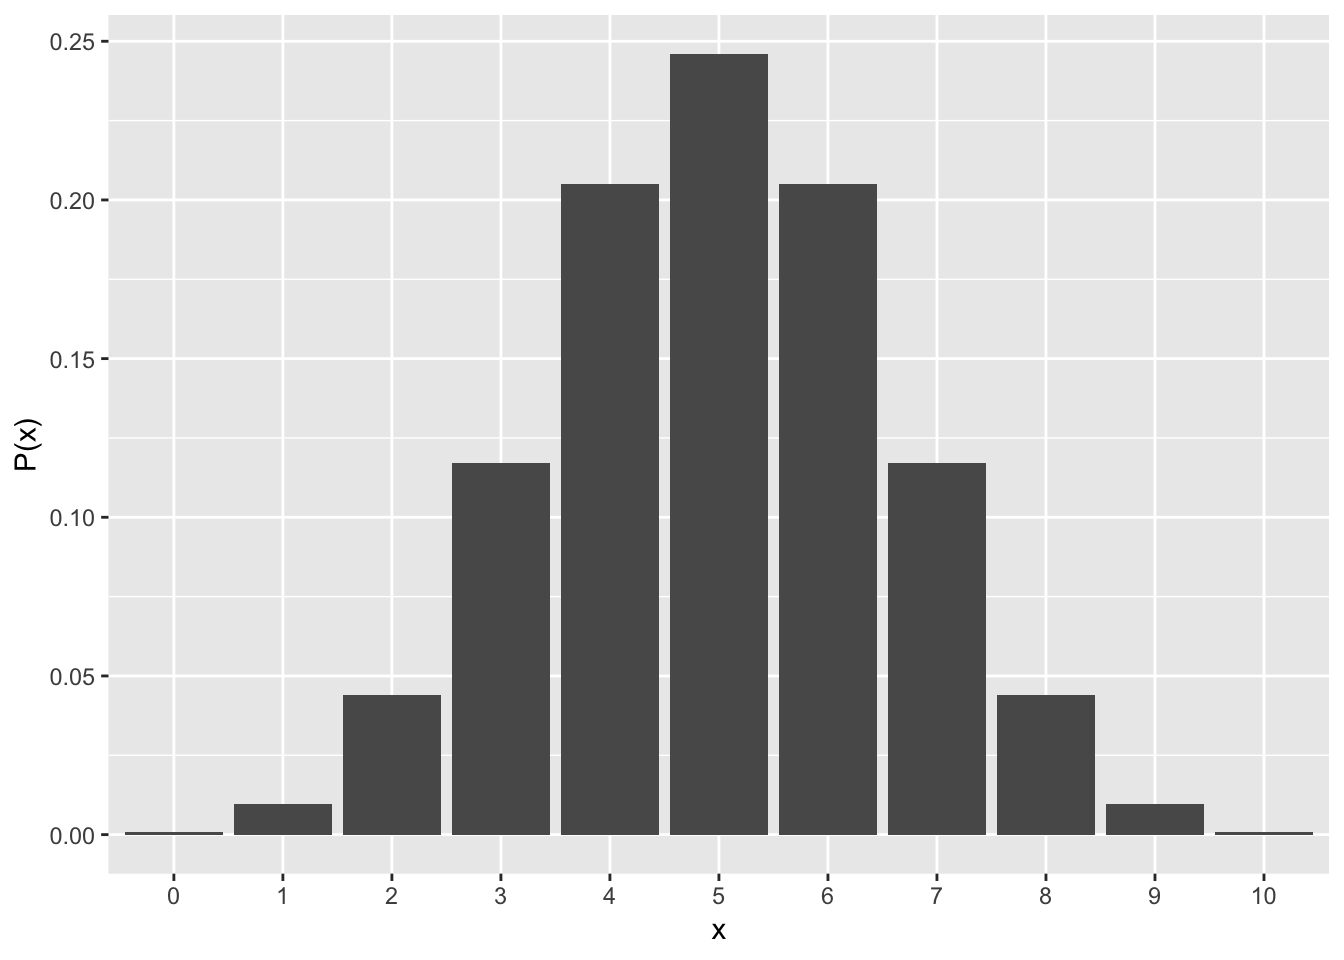
\includegraphics{Data-Analysis-for-Psychology_files/figure-latex/dbinom_2_plot_chap05-1.pdf}

\subsubsection{統計的仮説検定}

''理論的には'',表が出る回数Xは上の図のようになる(平均はnq = 10*0.5 =
5回)。

では,実際にコインを10回投げて表が出る回数をカウントしみたところ,表が2回しか出なかった。\\
この実験結果から,「このコインには歪みがあって,片一方の面だけが出やすい」と言ってもよいのか?

これを検討するために,表と裏それぞれが出る確率が等しいコインを投げる場合(すなわち,q=0.5)との比較を行い,今回の実験結果がどれくらいまれな事象と言えるのかを比較する。\\
このとき,研究者が検証したい仮説を\textbf{対立仮説}(alternative
hypothesis),対立仮説を検証するために比較の対象とする「偏りを仮定しない」仮説のことを\textbf{帰無仮説}(null
hypothesis)という。

では,今回の帰無仮説となるBinomial(n=10,
q=0.5)の分布を見てみよう。理論的には,表がx回出る確率pは,それぞれ以下のようになる。

\begin{Shaded}
\begin{Highlighting}[]
\NormalTok{d =}\StringTok{ }\KeywordTok{data.frame}\NormalTok{(}\DataTypeTok{x=}\DecValTok{0}\OperatorTok{:}\DecValTok{10}\NormalTok{, }\DataTypeTok{q=}\KeywordTok{dbinom}\NormalTok{(}\DataTypeTok{x=}\DecValTok{0}\OperatorTok{:}\DecValTok{10}\NormalTok{, }\DataTypeTok{size=}\DecValTok{10}\NormalTok{, }\DataTypeTok{prob=}\FloatTok{0.5}\NormalTok{))}
\NormalTok{d}
\end{Highlighting}
\end{Shaded}

\begin{verbatim}
##     x            q
## 1   0 0.0009765625
## 2   1 0.0097656250
## 3   2 0.0439453125
## 4   3 0.1171875000
## 5   4 0.2050781250
## 6   5 0.2460937500
## 7   6 0.2050781250
## 8   7 0.1171875000
## 9   8 0.0439453125
## 10  9 0.0097656250
## 11 10 0.0009765625
\end{verbatim}

表もしくは裏が出る回数が2回以下の場合の確率を計算すると,

\begin{Shaded}
\begin{Highlighting}[]
\KeywordTok{round}\NormalTok{(d}\OperatorTok{$}\NormalTok{q[}\DecValTok{1}\NormalTok{] }\OperatorTok{+}\StringTok{ }\NormalTok{d}\OperatorTok{$}\NormalTok{q[}\DecValTok{2}\NormalTok{] }\OperatorTok{+}\StringTok{ }\NormalTok{d}\OperatorTok{$}\NormalTok{q[}\DecValTok{3}\NormalTok{] }\OperatorTok{+}\StringTok{ }\NormalTok{d}\OperatorTok{$}\NormalTok{q[}\DecValTok{9}\NormalTok{] }\OperatorTok{+}\StringTok{ }\NormalTok{d}\OperatorTok{$}\NormalTok{q[}\DecValTok{10}\NormalTok{] }\OperatorTok{+}\StringTok{ }\NormalTok{d}\OperatorTok{$}\NormalTok{q[}\DecValTok{11}\NormalTok{], }\DecValTok{2}\NormalTok{)}
\end{Highlighting}
\end{Shaded}

\begin{verbatim}
## [1] 0.11
\end{verbatim}

となる。このことから,「フェアなコインを投げたら片一方の面だけが出る回数が2回以下の確率は
0.11
だ。こんなことはめったに起こらないから,このコインは歪んでいて片面だけが出やすい」と結論づけてよいのだろうか?

\begin{itemize}
\tightlist
\item
  「帰無仮説の前提のもとで,今回の結果が得られる確率」のことをp値(ピーち)と呼ぶ。
\item
  つまるところ,上述の問題は「p = 0.11
  は非常に小さい確率と評価してもよいのか」という問題である。「p値を小さい,もしくは大きい」と評価する基準となる確率を\textbf{有意水準}という。
\item
  一般的に有意水準には0.05(5\%)が使われる。なお,5%を基準とすることについては特に明確な根拠はない(研究の世界で合意されているからという以上の理由はない)。
\end{itemize}

帰無仮説(フェアなコインを投げる)の前提のもとでは,表が出る回数が2回以下の確率は
0.11
であり,5%より大きかった。すなわち,このコインはゆがんでいると結論付ける訳にはいかない,ということになる。

\begin{itemize}
\item
  ちなみに,今回のように「コインが表か裏かに関わらず,一方の面だけが出やすい」という対立仮説を検討する場合の検定は,\textbf{両側検定}という。仮に,今回の仮説で表と裏を区別するとして「表が出にくい」つまり「表が出る回数が2回以下の確率」を対象とする場合,このような検定を\textbf{片側検定}という。二項分布は左右対称の分布なので,両側p値は片側p値の2倍の値である(厳密には左右対称ではないのであくまで近似値)。多くの場合,両側検定を使うのが一般的。
\item
  Rならば,二項検定はbinom.test()関数で出来る。
\end{itemize}

\begin{Shaded}
\begin{Highlighting}[]
\CommentTok{#alternative = c("two.sided")は,両側検定をするためのオプション。alternativeを指定しなければ,出てくる結果はデフォルトで両側検定になる。}
\KeywordTok{binom.test}\NormalTok{(}\DataTypeTok{x =} \DecValTok{2}\NormalTok{, }\DataTypeTok{n =} \DecValTok{10}\NormalTok{, }\DataTypeTok{p =} \FloatTok{0.5}\NormalTok{, }\DataTypeTok{alternative =} \KeywordTok{c}\NormalTok{(}\StringTok{"two.sided"}\NormalTok{))}
\end{Highlighting}
\end{Shaded}

\begin{verbatim}
## 
##  Exact binomial test
## 
## data:  2 and 10
## number of successes = 2, number of trials = 10, p-value = 0.1094
## alternative hypothesis: true probability of success is not equal to 0.5
## 95 percent confidence interval:
##  0.02521073 0.55609546
## sample estimates:
## probability of success 
##                    0.2
\end{verbatim}

\begin{Shaded}
\begin{Highlighting}[]
\CommentTok{#alternative = c("less")は,片側検定をするためのオプション。2/10よりも低い確率を求めよということ。}
\KeywordTok{binom.test}\NormalTok{(}\DataTypeTok{x =} \DecValTok{2}\NormalTok{, }\DataTypeTok{n =} \DecValTok{10}\NormalTok{, }\DataTypeTok{p =} \FloatTok{0.5}\NormalTok{, }\DataTypeTok{alternative =} \KeywordTok{c}\NormalTok{(}\StringTok{"less"}\NormalTok{))}
\end{Highlighting}
\end{Shaded}

\begin{verbatim}
## 
##  Exact binomial test
## 
## data:  2 and 10
## number of successes = 2, number of trials = 10, p-value = 0.05469
## alternative hypothesis: true probability of success is less than 0.5
## 95 percent confidence interval:
##  0.0000000 0.5069013
## sample estimates:
## probability of success 
##                    0.2
\end{verbatim}

\begin{itemize}
\tightlist
\item
  2集団間の平均値の比較(t検定など)も,基本的に同じような考え方である。平均値に差がないと仮定したときの理論分布と比べて,実際に得られた値がどれくらい珍しいのかを検討する。
\end{itemize}

\subsection{第1種の過誤と第2種の過誤}\label{12}

\begin{itemize}
\tightlist
\item
  「帰無仮説が真なのに,帰無仮説を棄却してしまう誤り」のことを,第1種の過誤(type
  Ⅰ error)という。

  \begin{itemize}
  \tightlist
  \item
    本当は差がないのに,''差がある''と判断してしまう誤り。
  \item
    第1種の過誤を犯す確率をαと表現する。
  \item
    αは有意水準の値そのものである(α=0.05)。
  \end{itemize}
\item
  「帰無仮説が偽なのに,帰無仮説を採択してしまう」誤りのことを,第2種の過誤(type
  Ⅱ error)という。

  \begin{itemize}
  \tightlist
  \item
    本当は差があるのに,''差がない''と判断してしまう誤り。
  \item
    第2種の過誤を犯す確率をβと表現する。
  \end{itemize}
\item
  「帰無仮説が偽であるときに,正しく帰無仮説を棄却する確率」のことを''検定力''という。

  \begin{itemize}
  \tightlist
  \item
    差があるときに,''差がある''と正しく判断できる確率。\\
  \item
    検定力は1 -
    βで求められる(全体の確率から第2種の過誤を犯す確率を引いたもの)。
  \end{itemize}
\end{itemize}

表1\\
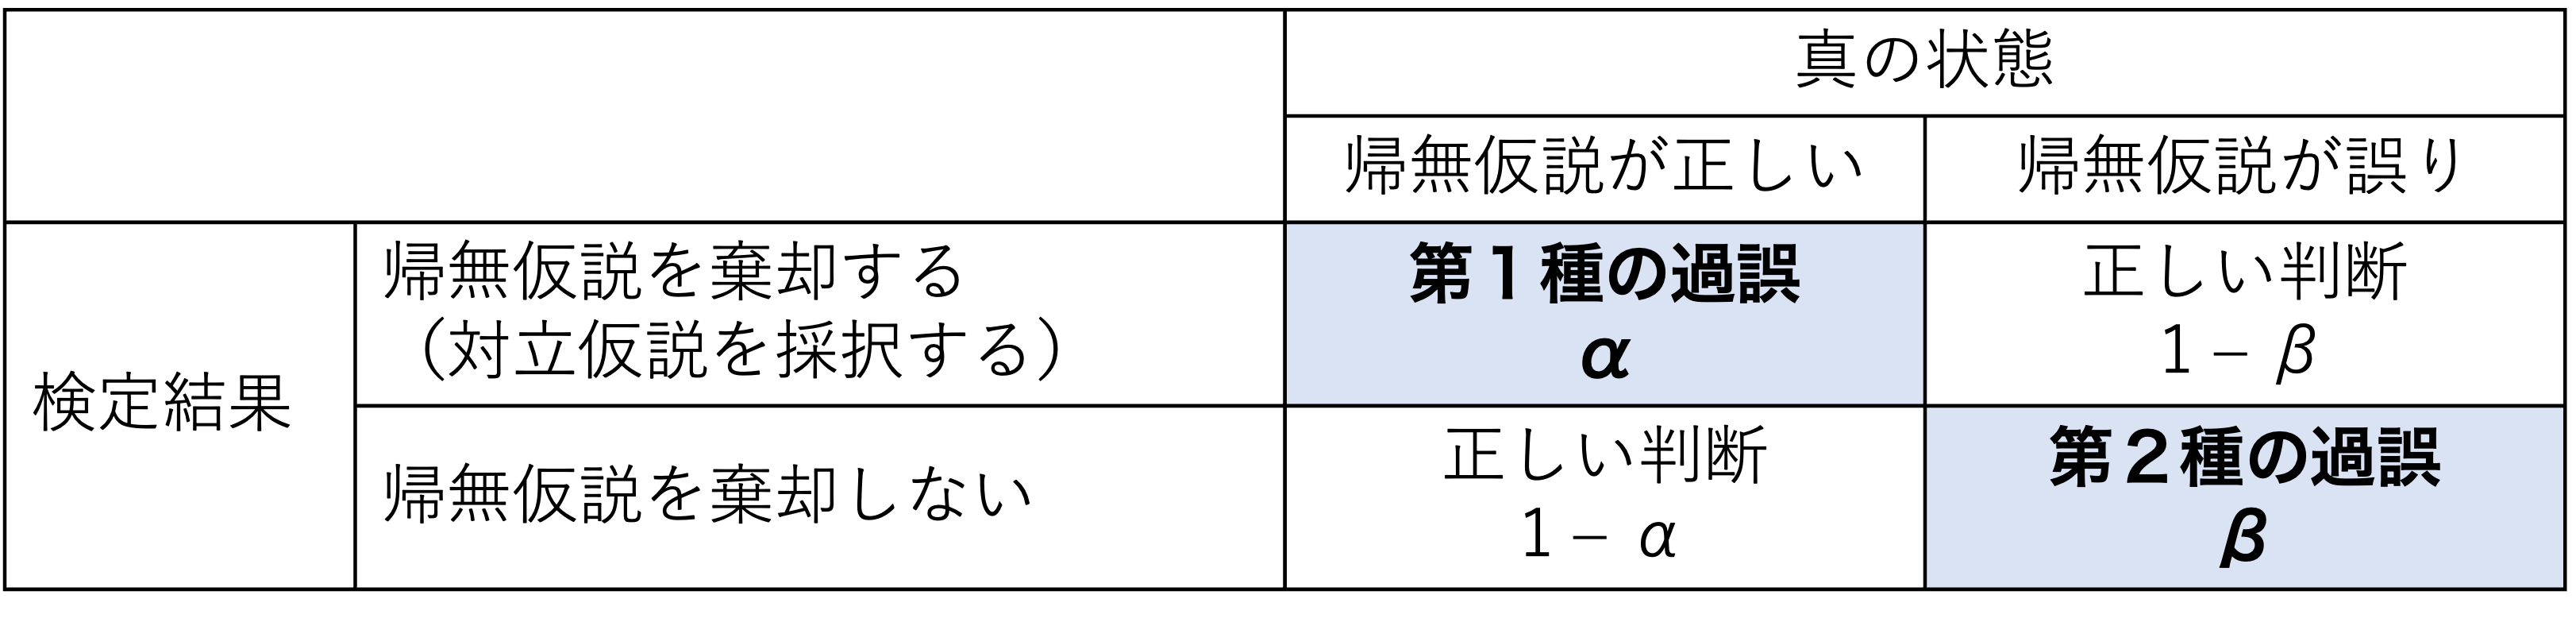
\includegraphics{05_table01.png}

\begin{itemize}
\tightlist
\item
  αとβはトレード・オフの関係にある。第Ⅰ種のエラーを避けようと思い有意水準を小さくすれば(例えばα=0.001とするなど),帰無仮説の棄却が厳しくなり,逆に第Ⅱ種のエラーを犯してしまう確率も高くなる(帰無仮説が偽であるにもかかわらず,棄却しない)。
\end{itemize}

\subsection{統計的検定の問題}

\subsubsection{p値}\label{p}

\begin{itemize}
\item
  有意水準は一般的に0.05が用いられる。0.05には特に根拠はない。
\item
  p値は標本数に依存する。標本数が多くなるほどp値は小さくなる。
\end{itemize}

例えば先程のコイン投げの例で,100回コインを投げて20回表が出た場合で(表が出る確率は0.2で先程の例と等しい),「フェアなコインと比べてこのコインはゆがんでいるか」を検討する。

\begin{Shaded}
\begin{Highlighting}[]
\KeywordTok{binom.test}\NormalTok{(}\DataTypeTok{x =} \DecValTok{20}\NormalTok{, }\DataTypeTok{n =} \DecValTok{100}\NormalTok{, }\DataTypeTok{p =} \FloatTok{0.5}\NormalTok{, }\DataTypeTok{alternative =} \KeywordTok{c}\NormalTok{(}\StringTok{"two.sided"}\NormalTok{))}
\end{Highlighting}
\end{Shaded}

\begin{verbatim}
## 
##  Exact binomial test
## 
## data:  20 and 100
## number of successes = 20, number of trials = 100, p-value =
## 1.116e-09
## alternative hypothesis: true probability of success is not equal to 0.5
## 95 percent confidence interval:
##  0.1266556 0.2918427
## sample estimates:
## probability of success 
##                    0.2
\end{verbatim}

そこで,p値ではなく,差の大きさそのものを表す指標である''効果量''というものが扱われている(詳しくは次回)。

\subsubsection{多重比較}

統計的検定を繰り返すと,有意な結果が生じる確率が増える。例えば,5\%水準で10回検定を行えば,少なくとも1回は帰無仮説を誤って棄却してしまう確率が0.4
になる。

\begin{Shaded}
\begin{Highlighting}[]
\CommentTok{#全ての確率から,「10回検定を行って全て正しい判断を行う」確率を差し引いたものが,少なくとも1回は誤った判断をしてしまう確率}
\DecValTok{1} \OperatorTok{-}\StringTok{ }\NormalTok{(}\DecValTok{1} \OperatorTok{-}\StringTok{ }\FloatTok{0.05}\NormalTok{)}\OperatorTok{^}\DecValTok{10}
\end{Highlighting}
\end{Shaded}

\begin{verbatim}
## [1] 0.4012631
\end{verbatim}

\begin{itemize}
\item
  このように複数回検定を行うことを多重比較という。有意な結果が出やすくなってしまうので,p値を調整する必要がある。
\item
  有名な多重比較補正は,ボンフェローニの補正である。10回検定を行うので,有意水準を元の0.05から0.05/10を基準とするといったかたちで調整する。
\end{itemize}

\begin{Shaded}
\begin{Highlighting}[]
\FloatTok{0.05}\OperatorTok{/}\DecValTok{10} \CommentTok{#つまり,p < 0.005でなければ「有意である」と結論しないという保守的な立場を取る}
\end{Highlighting}
\end{Shaded}

\begin{verbatim}
## [1] 0.005
\end{verbatim}

p.adjust()関数でも補正後のpを求めることができる。

\begin{Shaded}
\begin{Highlighting}[]
\CommentTok{#pには求めたp値,nには検定の回数を入れる。1回の検定でp=0.02だったとしても,「p = .20」と報告する。}
\KeywordTok{p.adjust}\NormalTok{(}\DataTypeTok{p =} \FloatTok{0.02}\NormalTok{, }\DataTypeTok{method =} \StringTok{"bonferroni"}\NormalTok{, }\DataTypeTok{n =} \DecValTok{10}\NormalTok{)}
\end{Highlighting}
\end{Shaded}

\begin{verbatim}
## [1] 0.2
\end{verbatim}

\subsection{練習問題}\label{-5}

\subsubsection{問1}\label{-10}

以下について,説明できるようにしておく。

\begin{itemize}
\tightlist
\item
  「帰無仮説」とはなにか?
\item
  「p値」とはなにか?
\item
  「第Ⅰ種の過誤」と「第Ⅱ種の過誤」とはなにか?
\end{itemize}

\subsubsection{問2}\label{-11}

\begin{itemize}
\item
  コインを100回投げて、表が51回出た。有意水準を5\%として統計的仮説検定をした場合,「このコインは歪みがない」という結論を出せるか?
\item
  コインを10,000回投げて、表が5,100回出た。有意水準を5\%として統計的仮説検定をした場合,「このコインは歪みがない」という結論を出せるか?
\end{itemize}

\section{t検定,分散分析}\label{t}

\begin{itemize}
\tightlist
\item
  これまで学んできた様々な統計的検定について復習をする。

  \begin{itemize}
  \tightlist
  \item
    t検定
  \item
    分散分析
  \end{itemize}
\end{itemize}

理論については深く掘り下げない(統計学の基礎授業で学んでいるので)。どの分析も前回学んだ「データが帰無仮説の分布に従うとしたときに,今回得られたデータが得られる確率がどれくらいまれか」を検討している点で共通している。様々な統計的検定の復習を通して,帰無仮説検定の考え方(p値とは何か)について理解する。

\subsection{準備}\label{-3}

必要なパッケージのインストールと乱数の種の指定をする。

\begin{Shaded}
\begin{Highlighting}[]
\KeywordTok{installed.packages}\NormalTok{(}\StringTok{"tidyverse"}\NormalTok{)}
\KeywordTok{library}\NormalTok{(tidyverse)}

\KeywordTok{set.seed}\NormalTok{(}\DecValTok{1234}\NormalTok{)}
\end{Highlighting}
\end{Shaded}

\subsection{t検定}\label{t}

連続量の変数を扱う検定の場合,t検定を使うのが一般的である。

\subsubsection{1標本のt検定}\label{t}

まずサンプルデータとして,平均0,
標準偏差1の正規分布からランダムに10個サンプルしたデータXを作る。\\
それぞれの平均と標準偏差を求めてみる。

\begin{Shaded}
\begin{Highlighting}[]
\KeywordTok{set.seed}\NormalTok{(}\DecValTok{1234}\NormalTok{)}
\NormalTok{X =}\StringTok{ }\KeywordTok{rnorm}\NormalTok{(}\DataTypeTok{n =} \DecValTok{10}\NormalTok{, }\DataTypeTok{mean =} \DecValTok{0}\NormalTok{, }\DataTypeTok{sd =} \DecValTok{1}\NormalTok{)}
\NormalTok{X}
\end{Highlighting}
\end{Shaded}

\begin{verbatim}
##  [1] -1.2070657  0.2774292  1.0844412 -2.3456977  0.4291247  0.5060559
##  [7] -0.5747400 -0.5466319 -0.5644520 -0.8900378
\end{verbatim}

\begin{Shaded}
\begin{Highlighting}[]
\KeywordTok{mean}\NormalTok{(X)}
\end{Highlighting}
\end{Shaded}

\begin{verbatim}
## [1] -0.3831574
\end{verbatim}

\begin{Shaded}
\begin{Highlighting}[]
\KeywordTok{sd}\NormalTok{(X)}
\end{Highlighting}
\end{Shaded}

\begin{verbatim}
## [1] 0.9957875
\end{verbatim}

このデータXから,帰無仮説「母集団の平均\(\mu\) = 0」を検定する。

\begin{Shaded}
\begin{Highlighting}[]
\CommentTok{#mu=0は入力しないでもOK}
\KeywordTok{t.test}\NormalTok{(X, }\DataTypeTok{mu=}\DecValTok{0}\NormalTok{)}
\end{Highlighting}
\end{Shaded}

\begin{verbatim}
## 
##  One Sample t-test
## 
## data:  X
## t = -1.2168, df = 9, p-value = 0.2546
## alternative hypothesis: true mean is not equal to 0
## 95 percent confidence interval:
##  -1.0955009  0.3291861
## sample estimates:
##  mean of x 
## -0.3831574
\end{verbatim}

t値,自由度(df),p値が出力される。\\
t値は以下の式から計算された統計量である。

\[
t = \frac{\bar{X} - \mu}{\sqrt{s^2/n}}
\]

Xが\(N(\mu, \sigma^2)\)に従う場合,tは自由度\(n-1\)のt分布に従う。

式にサンプルデータの平均と分散を入れてt値がt.test()で求めたものと一致するかを確かめてみよう。

\begin{Shaded}
\begin{Highlighting}[]
\NormalTok{t =}\StringTok{ }\NormalTok{(}\KeywordTok{mean}\NormalTok{(X) }\OperatorTok{-}\StringTok{ }\DecValTok{0}\NormalTok{) }\OperatorTok{/}\StringTok{ }\KeywordTok{sqrt}\NormalTok{(}\KeywordTok{var}\NormalTok{(X)}\OperatorTok{/}\DecValTok{10}\NormalTok{)}
\NormalTok{t}
\end{Highlighting}
\end{Shaded}

\begin{verbatim}
## [1] -1.216776
\end{verbatim}

Rならば,t.test()を使えばt値とp値,更に母集団の平均\(\mu\)の95\%信頼区間を出力してくれる。\\
出力結果から,\(N(\mu, \sigma^2)\)から今回観測されたデータX以上のtが得られる確率は0.25であるということを示している。この確率はまれといえるか(5\%未満か)について結論を下す。

\subsubsection{2標本の差のt検定(対応なし)}\label{t}

\begin{Shaded}
\begin{Highlighting}[]
\KeywordTok{set.seed}\NormalTok{(}\DecValTok{1234}\NormalTok{)}
\NormalTok{Value =}\StringTok{ }\KeywordTok{c}\NormalTok{(}\KeywordTok{rnorm}\NormalTok{(}\DataTypeTok{n =} \DecValTok{10}\NormalTok{, }\DataTypeTok{mean =} \DecValTok{0}\NormalTok{, }\DataTypeTok{sd =} \DecValTok{1}\NormalTok{), }\KeywordTok{rnorm}\NormalTok{(}\DataTypeTok{n =} \DecValTok{10}\NormalTok{, }\DataTypeTok{mean =} \DecValTok{1}\NormalTok{, }\DataTypeTok{sd =} \DecValTok{1}\NormalTok{))}
\NormalTok{Treatment =}\StringTok{ }\KeywordTok{c}\NormalTok{(}\KeywordTok{rep}\NormalTok{(}\StringTok{"X"}\NormalTok{, }\DecValTok{10}\NormalTok{), }\KeywordTok{rep}\NormalTok{(}\StringTok{"Y"}\NormalTok{, }\DecValTok{10}\NormalTok{))}
\NormalTok{sample_data =}\StringTok{ }\KeywordTok{data.frame}\NormalTok{(}\DataTypeTok{Treatment =}\NormalTok{ Treatment, }\DataTypeTok{Value =}\NormalTok{ Value)}


\NormalTok{sample_data }\OperatorTok\StringTok{ }\KeywordTok{group_by}\NormalTok{(Treatment) }\OperatorTok
\StringTok{  }\KeywordTok{summarise}\NormalTok{(}\DataTypeTok{Mean =} \KeywordTok{mean}\NormalTok{(Value), }\DataTypeTok{SD =} \KeywordTok{sd}\NormalTok{(Value), }\DataTypeTok{N =} \KeywordTok{length}\NormalTok{(Value))}
\end{Highlighting}
\end{Shaded}

\begin{verbatim}
## # A tibble: 2 x 4
##   Treatment   Mean    SD     N
##   <fct>      <dbl> <dbl> <int>
## 1 X         -0.383 0.996    10
## 2 Y          0.882 1.07     10
\end{verbatim}

Xのサンプル数をm, Yのサンプル数をnとする。

\[
t = \frac{\bar{X} - \bar{Y}}{\sqrt{s^2_{X}/m+s^2_{Y}/n))}}
\]
XとYは同じ\(N(\mu, \sigma^2)\)に従う時,t値は自由度\(m+n-2\)のt分布に従う。\\
つまり,同じ母集団からXとYが抽出されたと仮定した時(\(\bar{X} - \bar{Y}\)),今回のデータが得られる確率がどのくらいまれであるかを検討する。

\begin{Shaded}
\begin{Highlighting}[]
\CommentTok{#2つの標本の母分散が等しいと仮定できない場合}
\CommentTok{#ウェルチの検定(Welch's t-test)と呼ばれる検定}
\KeywordTok{t.test}\NormalTok{(}\DataTypeTok{data =}\NormalTok{ sample_data, Value }\OperatorTok{~}\StringTok{ }\NormalTok{Treatment, }\DataTypeTok{paired =}\NormalTok{ F)}
\end{Highlighting}
\end{Shaded}

\begin{verbatim}
## 
##  Welch Two Sample t-test
## 
## data:  Value by Treatment
## t = -2.7404, df = 17.914, p-value = 0.01349
## alternative hypothesis: true difference in means is not equal to 0
## 95 percent confidence interval:
##  -2.2351190 -0.2948544
## sample estimates:
## mean in group X mean in group Y 
##      -0.3831574       0.8818293
\end{verbatim}

\begin{Shaded}
\begin{Highlighting}[]
\CommentTok{#2つの標本の母分散が等しいと仮定する場合}
\CommentTok{#var.equal = Tを指定する(デフォルトでvar.equal = Fとなる)}
\KeywordTok{t.test}\NormalTok{(}\DataTypeTok{data =}\NormalTok{ sample_data, Value }\OperatorTok{~}\StringTok{ }\NormalTok{Treatment, }\DataTypeTok{paired =}\NormalTok{ F, }\DataTypeTok{var.equal =}\NormalTok{ T)}
\end{Highlighting}
\end{Shaded}

\begin{verbatim}
## 
##  Two Sample t-test
## 
## data:  Value by Treatment
## t = -2.7404, df = 18, p-value = 0.01344
## alternative hypothesis: true difference in means is not equal to 0
## 95 percent confidence interval:
##  -2.2347852 -0.2951882
## sample estimates:
## mean in group X mean in group Y 
##      -0.3831574       0.8818293
\end{verbatim}

等分散を仮定した場合しない場合いずれも,それぞれの平均の間に有意な差があるといえる。

\begin{itemize}
\tightlist
\item
  論文などにt検定の結果を報告するときは一般的に,「t(17.9)=2.74, p =
  0.01」と書く。つまり,t値,自由度,p値を報告する。
\item
  一般的に2つの標本の母分散は不明であるので,それらが等しいかどうかも不明である。なので,等分散を仮定しないt検定をしておくほうが保守的である。
\end{itemize}

\subsubsection{2標本の差のt検定(対応あり)}\label{t}

\begin{Shaded}
\begin{Highlighting}[]
\KeywordTok{t.test}\NormalTok{(}\DataTypeTok{data =}\NormalTok{ sample_data, Value }\OperatorTok{~}\StringTok{ }\NormalTok{Treatment, }\DataTypeTok{paired =}\NormalTok{ T)}
\end{Highlighting}
\end{Shaded}

\begin{verbatim}
## 
##  Paired t-test
## 
## data:  Value by Treatment
## t = -2.5283, df = 9, p-value = 0.03233
## alternative hypothesis: true difference in means is not equal to 0
## 95 percent confidence interval:
##  -2.3968339 -0.1331395
## sample estimates:
## mean of the differences 
##               -1.264987
\end{verbatim}

\begin{Shaded}
\begin{Highlighting}[]
\CommentTok{#なお,等分散を仮定する場合はvar.equal = Tを指定する。}
\KeywordTok{t.test}\NormalTok{(}\DataTypeTok{data =}\NormalTok{ sample_data, Value }\OperatorTok{~}\StringTok{ }\NormalTok{Treatment, }\DataTypeTok{paired =}\NormalTok{ T, }\DataTypeTok{var.equal =}\NormalTok{ T)}
\end{Highlighting}
\end{Shaded}

\begin{verbatim}
## 
##  Paired t-test
## 
## data:  Value by Treatment
## t = -2.5283, df = 9, p-value = 0.03233
## alternative hypothesis: true difference in means is not equal to 0
## 95 percent confidence interval:
##  -2.3968339 -0.1331395
## sample estimates:
## mean of the differences 
##               -1.264987
\end{verbatim}

\subsection{分散分析}

t検定で比較できるのは2群までである。3群以上の間で平均値の比較を行いたい場合は,分散分析(ANOVA)を行う。

\subsubsection{一要因の分散分析}

\begin{Shaded}
\begin{Highlighting}[]
\CommentTok{#サンプルデータ}
\NormalTok{Y1 =}\StringTok{ }\KeywordTok{c}\NormalTok{(}\DecValTok{1}\NormalTok{, }\DecValTok{2}\NormalTok{, }\DecValTok{3}\NormalTok{)}
\NormalTok{Y2 =}\StringTok{ }\KeywordTok{c}\NormalTok{(}\DecValTok{5}\NormalTok{, }\DecValTok{7}\NormalTok{, }\DecValTok{5}\NormalTok{)}
\NormalTok{Y3 =}\StringTok{ }\KeywordTok{c}\NormalTok{(}\DecValTok{5}\NormalTok{, }\DecValTok{4}\NormalTok{, }\DecValTok{2}\NormalTok{)}
\NormalTok{Value =}\StringTok{ }\KeywordTok{c}\NormalTok{(Y1, Y2, Y3)}
\NormalTok{Treatment =}\StringTok{ }\KeywordTok{factor}\NormalTok{(}\KeywordTok{c}\NormalTok{(}\DecValTok{1}\NormalTok{, }\DecValTok{1}\NormalTok{, }\DecValTok{1}\NormalTok{, }\DecValTok{2}\NormalTok{, }\DecValTok{2}\NormalTok{, }\DecValTok{2}\NormalTok{, }\DecValTok{3}\NormalTok{, }\DecValTok{3}\NormalTok{, }\DecValTok{3}\NormalTok{))}
\NormalTok{sample_data2 =}\StringTok{ }\KeywordTok{data.frame}\NormalTok{(}\DataTypeTok{Treatment =}\NormalTok{ Treatment, }\DataTypeTok{Value =}\NormalTok{ Value)}
\NormalTok{sample_data2}
\end{Highlighting}
\end{Shaded}

\begin{verbatim}
##   Treatment Value
## 1         1     1
## 2         1     2
## 3         1     3
## 4         2     5
## 5         2     7
## 6         2     5
## 7         3     5
## 8         3     4
## 9         3     2
\end{verbatim}

それぞれ3つのグループ(X = 1, 2, or 3)で変数Yを取ったとする。
グループごとの平均値などは,以下のようになっている。これら3つのグループの間で平均値に差があるのかを検定する。

\begin{Shaded}
\begin{Highlighting}[]
\NormalTok{sample_data2 }\OperatorTok\StringTok{ }\NormalTok{dplyr}\OperatorTok{::}\KeywordTok{group_by}\NormalTok{(Treatment) }\OperatorTok\StringTok{ }
\StringTok{  }\NormalTok{dplyr}\OperatorTok{::}\KeywordTok{summarise}\NormalTok{(}\DataTypeTok{Mean =} \KeywordTok{mean}\NormalTok{(Value), }\DataTypeTok{SD =} \KeywordTok{sd}\NormalTok{(Value), }\DataTypeTok{N =} \KeywordTok{length}\NormalTok{(Value))}
\end{Highlighting}
\end{Shaded}

\begin{verbatim}
## # A tibble: 3 x 4
##   Treatment  Mean    SD     N
##   <fct>     <dbl> <dbl> <int>
## 1 1          2     1        3
## 2 2          5.67  1.15     3
## 3 3          3.67  1.53     3
\end{verbatim}

\begin{Shaded}
\begin{Highlighting}[]
\NormalTok{result_anova =}\StringTok{ }\KeywordTok{aov}\NormalTok{(}\DataTypeTok{data =}\NormalTok{ sample_data2, Value }\OperatorTok{~}\StringTok{ }\NormalTok{Treatment)}
\KeywordTok{summary}\NormalTok{(result_anova)}
\end{Highlighting}
\end{Shaded}

\begin{verbatim}
##             Df Sum Sq Mean Sq F value Pr(>F)  
## Treatment    2 20.222  10.111     6.5 0.0315 *
## Residuals    6  9.333   1.556                 
## ---
## Signif. codes:  0 '***' 0.001 '**' 0.01 '*' 0.05 '.' 0.1 ' ' 1
\end{verbatim}

\begin{Shaded}
\begin{Highlighting}[]
\CommentTok{#以下でも同じ結果が出る}
\KeywordTok{oneway.test}\NormalTok{(}\DataTypeTok{data =}\NormalTok{ sample_data2, Value }\OperatorTok{~}\StringTok{ }\NormalTok{Treatment, }\DataTypeTok{var.equal =} \OtherTok{TRUE}\NormalTok{)}
\end{Highlighting}
\end{Shaded}

\begin{verbatim}
## 
##  One-way analysis of means
## 
## data:  Value and Treatment
## F = 6.5, num df = 2, denom df = 6, p-value = 0.03149
\end{verbatim}

\begin{Shaded}
\begin{Highlighting}[]
\CommentTok{#lm関数でも分散分析表を出せる(ただし,lm関数を使った場合ではTukeyHSD()は使えないので注意。多重比較をしたい場合はaov()を使う。}
\NormalTok{result_anova_}\DecValTok{2}\NormalTok{ =}\StringTok{ }\KeywordTok{lm}\NormalTok{(}\DataTypeTok{data =}\NormalTok{ sample_data2, Value}\OperatorTok{~}\NormalTok{Treatment)}
\KeywordTok{anova}\NormalTok{(result_anova_}\DecValTok{2}\NormalTok{)}
\end{Highlighting}
\end{Shaded}

\begin{verbatim}
## Analysis of Variance Table
## 
## Response: Value
##           Df  Sum Sq Mean Sq F value  Pr(>F)  
## Treatment  2 20.2222 10.1111     6.5 0.03149 *
## Residuals  6  9.3333  1.5556                  
## ---
## Signif. codes:  0 '***' 0.001 '**' 0.01 '*' 0.05 '.' 0.1 ' ' 1
\end{verbatim}

\begin{itemize}
\item
  ここでは分散分析の理論の詳細は省略する。
  簡単に説明すると,分散分析ではグループ間の分散がグループ内の分散と比べて大きい確率を求めて,群の間で平均値に差があるかを検定する。
\item
  回帰分析(正確には線形モデルと呼ばれる統計解析の枠組み)でも,分散分析と同様の目的の検定を行うことができる。\\
\item
  分散分析は要因の数やそれぞれの要因の対応ありなしによって,やり方が複雑になる(例えばテストの成績に対して,男女,学年,科目によってどう差があるかを検討するなど)。線形モデルならば,もっとシンプルに行うことができる。\\
\item
  分散分析の結果を論文で報告するときは,「F(2, 6) = 2.26, p =
  .19」といったように報告する。
\item
  anova()関数では,逐次平方和(Type Ⅰ
  SS)が出力される(要因の各セルのデータ数にかたよりがある場合,独立変数を投入した順序(x1,
  x2とx2,
  x1)で平方和の値の計算結果が異なる場合がある)。調整平方和(Type
  Ⅱ,Type
  Ⅲ)を出したいときは,carパッケージのAnova()関数など別のパッケージが必要になる。
\end{itemize}

\subsubsection{多重比較}\label{-1}

\begin{itemize}
\item
  「3つのグループの間で平均値に差がない」という帰無仮説が棄却された場合,どのグループの間に有意な差があるのかを検定する必要がある。このサンプルデータの場合,グループ1とグループ2,グループ2とグループ3,グループ1とグループ3との間,計3つの組み合わせで平均値の比較を行う。つまり,t検定を3回行って条件間の比較をする。
\item
  ただし,第5回でも述べたように,統計的検定を繰り返し行う(多重比較)と第一種のエラーを犯す確率が増える。t検定で出てきたp値をそのまま報告するのではなく,多重比較の問題を考慮した上でp値に補正をかける(p値を過大に評価し直す)必要がある。
\item
  多重比較の補正法には,いくつかの方法がある。

  \begin{itemize}
  \tightlist
  \item
    ボンフェローニ(Bonferroni)の方法:
    p値を比較の回数分かけて過大に評価する\\
  \item
    チューキー(Tukey)の方法\\
  \item
    ホルム(Holm)の方法
  \end{itemize}
\item
  多重比較の補正を行うときは,pairwise.t.test関数を使う。各群間の比較について,補正後のp値が出力される。
\end{itemize}

\begin{Shaded}
\begin{Highlighting}[]
\KeywordTok{pairwise.t.test}\NormalTok{(sample_data2}\OperatorTok{$}\NormalTok{Value, }\DataTypeTok{g =}\NormalTok{ sample_data2}\OperatorTok{$}\NormalTok{Treatment, }\DataTypeTok{p.adjust.method =} \StringTok{"bonferroni"}\NormalTok{) }\CommentTok{#gがグループを意味する変数,p.adjust.methodに補正方法を指定する。}
\end{Highlighting}
\end{Shaded}

\begin{verbatim}
## 
##  Pairwise comparisons using t tests with pooled SD 
## 
## data:  sample_data2$Value and sample_data2$Treatment 
## 
##   1     2    
## 2 0.034 -    
## 3 0.458 0.291
## 
## P value adjustment method: bonferroni
\end{verbatim}

\begin{Shaded}
\begin{Highlighting}[]
\KeywordTok{pairwise.t.test}\NormalTok{(sample_data2}\OperatorTok{$}\NormalTok{Value, }\DataTypeTok{g =}\NormalTok{ sample_data2}\OperatorTok{$}\NormalTok{Treatment) }\CommentTok{#オプションに何も指定しないと,ホルムの方法の結果が出力される。ボンフェローニの方法は保守的すぎるので,他の方法の方が好まれる。}
\end{Highlighting}
\end{Shaded}

\begin{verbatim}
## 
##  Pairwise comparisons using t tests with pooled SD 
## 
## data:  sample_data2$Value and sample_data2$Treatment 
## 
##   1     2    
## 2 0.034 -    
## 3 0.194 0.194
## 
## P value adjustment method: holm
\end{verbatim}

\begin{itemize}
\tightlist
\item
  よく使われるチューキーの方法を使う場合は,TukeyHSD()関数が用意されている。
\end{itemize}

\begin{Shaded}
\begin{Highlighting}[]
\KeywordTok{TukeyHSD}\NormalTok{(result_anova) }\CommentTok{#TukeyHSD()に,分散分析表の結果を入れる}
\end{Highlighting}
\end{Shaded}

\begin{verbatim}
##   Tukey multiple comparisons of means
##     95% family-wise confidence level
## 
## Fit: aov(formula = Value ~ Treatment, data = sample_data2)
## 
## $Treatment
##          diff        lwr      upr     p adj
## 2-1  3.666667  0.5420889 6.791244 0.0263939
## 3-1  1.666667 -1.4579111 4.791244 0.3023895
## 3-2 -2.000000 -5.1245777 1.124578 0.2019189
\end{verbatim}

\subsection{まとめ}

\begin{itemize}
\tightlist
\item
  統計学の基礎の復習として,これまで学んだ統計解析(+α)の復習をしてきた。いずれも考え方は共通していて,「データから求めた統計量が帰無仮説に従うとしたときに,今回のデータよりもまれな事象が得られる確率(p値)」を求めている。\\
\item
  更に,これまで学んできた統計手法は統計モデルというかたちで包括的に理解することができる。詳しくはまた後日学ぶ「一般化線形モデル」の回で扱う。t検定,分散分析なども,「一般化線形モデル」の中に含まれる。「一般化線形モデル」を理解すれば,様々なデータに対して適切な分析を行うことができるようになる。\\
\item
  次回はp値を基準として結論を出す帰無仮説検定が抱える問題について扱う。
\end{itemize}

\subsection{練習問題}\label{-6}

\subsubsection{問1}\label{-12}

\begin{itemize}
\item
  以下のプログラムを読み込む。
\item
  あるサプリメントにダイエットの効果があるかを検討するために,10名を対象に実験を行った。それぞれの参加者にサプリメントを投与する前(before)と投与した後(after)で体重を測定した(架空のデータである)。
\end{itemize}

\begin{Shaded}
\begin{Highlighting}[]
\NormalTok{before =}\StringTok{ }\KeywordTok{c}\NormalTok{(}\FloatTok{37.93}\NormalTok{, }\FloatTok{52.77}\NormalTok{, }\FloatTok{60.84}\NormalTok{, }\FloatTok{26.54}\NormalTok{, }\FloatTok{54.29}\NormalTok{, }\FloatTok{55.06}\NormalTok{, }\FloatTok{44.25}\NormalTok{, }\FloatTok{44.53}\NormalTok{, }\FloatTok{44.36}\NormalTok{, }\FloatTok{41.1}\NormalTok{)}
\NormalTok{after =}\StringTok{ }\KeywordTok{c}\NormalTok{(}\FloatTok{57.84}\NormalTok{, }\FloatTok{50.02}\NormalTok{, }\FloatTok{53.36}\NormalTok{, }\FloatTok{65.97}\NormalTok{, }\FloatTok{79.39}\NormalTok{, }\FloatTok{63.35}\NormalTok{, }\FloatTok{57.33}\NormalTok{, }\FloatTok{51.33}\NormalTok{, }\FloatTok{52.44}\NormalTok{, }\FloatTok{101.24}\NormalTok{)}
\NormalTok{Value =}\StringTok{ }\KeywordTok{c}\NormalTok{(before, after)}
\NormalTok{Treatment =}\StringTok{ }\KeywordTok{c}\NormalTok{(}\KeywordTok{rep}\NormalTok{(}\StringTok{"before"}\NormalTok{, }\DecValTok{10}\NormalTok{), }\KeywordTok{rep}\NormalTok{(}\StringTok{"after"}\NormalTok{, }\DecValTok{10}\NormalTok{))}
\NormalTok{Subject =}\StringTok{ }\KeywordTok{c}\NormalTok{(}\KeywordTok{c}\NormalTok{(}\DecValTok{1}\OperatorTok{:}\DecValTok{10}\NormalTok{), }\KeywordTok{c}\NormalTok{(}\DecValTok{1}\OperatorTok{:}\DecValTok{10}\NormalTok{))}
\NormalTok{sample_}\DecValTok{1}\NormalTok{ =}\StringTok{ }\KeywordTok{data.frame}\NormalTok{(}\DataTypeTok{Subject =}\NormalTok{ Subject, }\DataTypeTok{Treatment =}\NormalTok{ Treatment, }\DataTypeTok{Value =}\NormalTok{ Value)}
\NormalTok{sample_}\DecValTok{1}
\end{Highlighting}
\end{Shaded}

\begin{verbatim}
##    Subject Treatment  Value
## 1        1    before  37.93
## 2        2    before  52.77
## 3        3    before  60.84
## 4        4    before  26.54
## 5        5    before  54.29
## 6        6    before  55.06
## 7        7    before  44.25
## 8        8    before  44.53
## 9        9    before  44.36
## 10      10    before  41.10
## 11       1     after  57.84
## 12       2     after  50.02
## 13       3     after  53.36
## 14       4     after  65.97
## 15       5     after  79.39
## 16       6     after  63.35
## 17       7     after  57.33
## 18       8     after  51.33
## 19       9     after  52.44
## 20      10     after 101.24
\end{verbatim}

\begin{itemize}
\tightlist
\item
  投与前と投与後それぞれについて,体重の平均値及び標準偏差を求めて報告せよ。\\
\item
  このサプリメントの投与により体重が変化したかについてt検定(等分散を仮定しない)で検討し,結果について報告するとともに結論を述べよ。
\end{itemize}

\subsubsection{問2}\label{-13}

\begin{itemize}
\item
  以下のプログラムを読み込む。
\item
  ある教授法に児童の学力向上の効果があるかを検討した。学校Bにはその教授法を実施し,学校Aには何もしなかった。その後,学校Aと学校Bそれぞれ10人の生徒に学力テストを行った。A,Bそれぞれが学校A,Bそれぞれの生徒の成績である(架空のデータである)。
\end{itemize}

\begin{Shaded}
\begin{Highlighting}[]
\NormalTok{A =}\StringTok{ }\KeywordTok{c}\NormalTok{(}\DecValTok{38}\NormalTok{, }\DecValTok{53}\NormalTok{, }\DecValTok{61}\NormalTok{, }\DecValTok{27}\NormalTok{, }\DecValTok{54}\NormalTok{, }\DecValTok{55}\NormalTok{, }\DecValTok{44}\NormalTok{, }\DecValTok{45}\NormalTok{, }\DecValTok{44}\NormalTok{, }\DecValTok{41}\NormalTok{)}
\NormalTok{B =}\StringTok{ }\KeywordTok{c}\NormalTok{(}\DecValTok{48}\NormalTok{, }\DecValTok{40}\NormalTok{, }\DecValTok{43}\NormalTok{, }\DecValTok{56}\NormalTok{, }\DecValTok{69}\NormalTok{, }\DecValTok{53}\NormalTok{, }\DecValTok{47}\NormalTok{, }\DecValTok{41}\NormalTok{, }\DecValTok{42}\NormalTok{, }\DecValTok{91}\NormalTok{)}
\NormalTok{Value =}\StringTok{ }\KeywordTok{c}\NormalTok{(A, B)}
\NormalTok{Treatment =}\StringTok{ }\KeywordTok{c}\NormalTok{(}\KeywordTok{rep}\NormalTok{(}\StringTok{"A"}\NormalTok{, }\DecValTok{10}\NormalTok{), }\KeywordTok{rep}\NormalTok{(}\StringTok{"B"}\NormalTok{, }\DecValTok{10}\NormalTok{))}
\NormalTok{sample_}\DecValTok{2}\NormalTok{ =}\StringTok{ }\KeywordTok{data.frame}\NormalTok{(}\DataTypeTok{Treatment =}\NormalTok{ Treatment, }\DataTypeTok{Value =}\NormalTok{ Value)}
\NormalTok{sample_}\DecValTok{2}
\end{Highlighting}
\end{Shaded}

\begin{verbatim}
##    Treatment Value
## 1          A    38
## 2          A    53
## 3          A    61
## 4          A    27
## 5          A    54
## 6          A    55
## 7          A    44
## 8          A    45
## 9          A    44
## 10         A    41
## 11         B    48
## 12         B    40
## 13         B    43
## 14         B    56
## 15         B    69
## 16         B    53
## 17         B    47
## 18         B    41
## 19         B    42
## 20         B    91
\end{verbatim}

\begin{itemize}
\tightlist
\item
  学校Aと学校Bそれぞれについて,テストの得点の平均値及び標準偏差を求めて報告せよ。\\
\item
  この教授法に成績向上があったかどうかについてt検定(等分散を仮定しない)で検討し,結果について報告するとともに結論を述べよ。
\end{itemize}

\subsubsection{問3}\label{-14}

\begin{itemize}
\item
  以下のプログラムを読み込む。
\item
  A県, B県,
  C県のそれぞれで学力テストを行った。各県で10名の生徒の成績を集計し,県(prefecture)ごとの得点(score)である(架空のデータである)。A,Bそれぞれが学校A,Bそれぞれの生徒の成績である。
\end{itemize}

\begin{Shaded}
\begin{Highlighting}[]
\NormalTok{Value =}\StringTok{ }\KeywordTok{c}\NormalTok{(}\DecValTok{38}\NormalTok{, }\DecValTok{40}\NormalTok{, }\DecValTok{58}\NormalTok{, }\DecValTok{27}\NormalTok{, }\DecValTok{54}\NormalTok{, }\DecValTok{55}\NormalTok{, }\DecValTok{44}\NormalTok{, }\DecValTok{45}\NormalTok{, }\DecValTok{44}\NormalTok{, }\DecValTok{41}\NormalTok{, }\DecValTok{44}\NormalTok{, }\DecValTok{38}\NormalTok{, }\DecValTok{41}\NormalTok{, }\DecValTok{51}\NormalTok{, }\DecValTok{62}\NormalTok{, }\DecValTok{49}\NormalTok{, }\DecValTok{44}\NormalTok{, }\DecValTok{39}\NormalTok{, }\DecValTok{40}\NormalTok{, }\DecValTok{79}\NormalTok{, }\DecValTok{61}\NormalTok{, }\DecValTok{55}\NormalTok{, }\DecValTok{56}\NormalTok{, }\DecValTok{65}\NormalTok{, }\DecValTok{53}\NormalTok{, }\DecValTok{46}\NormalTok{, }\DecValTok{66}\NormalTok{, }\DecValTok{50}\NormalTok{, }\DecValTok{60}\NormalTok{, }\DecValTok{51}\NormalTok{)}
\NormalTok{Prefecture =}\StringTok{ }\KeywordTok{c}\NormalTok{(}\KeywordTok{rep}\NormalTok{(}\StringTok{"A"}\NormalTok{, }\DecValTok{10}\NormalTok{), }\KeywordTok{rep}\NormalTok{(}\StringTok{"B"}\NormalTok{, }\DecValTok{10}\NormalTok{), }\KeywordTok{rep}\NormalTok{(}\StringTok{"C"}\NormalTok{, }\DecValTok{10}\NormalTok{))}
\NormalTok{sample_}\DecValTok{3}\NormalTok{ =}\StringTok{ }\KeywordTok{data.frame}\NormalTok{(}\DataTypeTok{Prefecture =}\NormalTok{ Prefecture, }\DataTypeTok{Value =}\NormalTok{ Value)}
\NormalTok{sample_}\DecValTok{3}
\end{Highlighting}
\end{Shaded}

\begin{verbatim}
##    Prefecture Value
## 1           A    38
## 2           A    40
## 3           A    58
## 4           A    27
## 5           A    54
## 6           A    55
## 7           A    44
## 8           A    45
## 9           A    44
## 10          A    41
## 11          B    44
## 12          B    38
## 13          B    41
## 14          B    51
## 15          B    62
## 16          B    49
## 17          B    44
## 18          B    39
## 19          B    40
## 20          B    79
## 21          C    61
## 22          C    55
## 23          C    56
## 24          C    65
## 25          C    53
## 26          C    46
## 27          C    66
## 28          C    50
## 29          C    60
## 30          C    51
\end{verbatim}

\begin{itemize}
\tightlist
\item
  A県,B県,C県の成績の平均値及び標準偏差は以下の通りである。
\end{itemize}

\begin{tabular}{l|r|r|r}
\hline
Prefecture & Mean & SD & N\\
\hline
A & 44.6 & 9.215928 & 10\\
\hline
B & 48.7 & 12.858633 & 10\\
\hline
C & 56.3 & 6.600505 & 10\\
\hline
\end{tabular}

\begin{itemize}
\item
  県によって学力に違いがあるかについて一元配置分散分析で検討し,結果について報告するとともに結論を述べよ。
\item
  県の間で学力に有意差が見られた場合は,どの県とどの県との間に有意差があるかをホルムの方法で確認し,結果について報告せよ。
\end{itemize}

\section{統計的帰無仮説検定の問題}

\begin{itemize}
\tightlist
\item
  以下の4つの関係を理解し,統計的帰無仮説検定が抱える問題点について理解する。

  \begin{itemize}
  \tightlist
  \item
    有意水準
  \item
    効果量
  \item
    検定力
  \item
    サンプルサイズ
  \end{itemize}
\item
  信頼区間について学ぶ
\end{itemize}

\subsection{準備}\label{-4}

tidyverseとpwrパッケージをインストールして使う。

\begin{Shaded}
\begin{Highlighting}[]
\KeywordTok{install.packages}\NormalTok{(}\StringTok{"pwr"}\NormalTok{, }\StringTok{"tidyverse"}\NormalTok{)}
\KeywordTok{library}\NormalTok{(pwr)}
\KeywordTok{library}\NormalTok{(tidyverse)}
\end{Highlighting}
\end{Shaded}

\subsection{p値の問題}\label{p}

\subsubsection{第Ⅰ種の過誤}

\begin{itemize}
\tightlist
\item
  第Ⅰ種の過誤(α)とは,「帰無仮説が真なのに,帰無仮説を棄却する誤り」であった。第Ⅰ種の過誤を犯す確率は,有意水準として設定する確率である。
\item
  有意水準は一般的に5\%が用いられる。第Ⅰ種の過誤を犯す確率を少なくするためにできるだけ小さい確率ということで,慣習として5\%とされている(20回に1回くらいの誤りは許す)。
\end{itemize}

\subsubsection{p値と標本数の関係}\label{p}

\begin{itemize}
\item
  しかし,p値は標本数に依存する。標本数が多くなるほどp値は小さくなる。
\item
  例えばコイン投げて表が出る回数をカウントする実験を行う。10回コインを投げて2回表が出た場合,100回コインを投げて20回表が出た場合それぞれについて(表が出た割合はどちらも0.2),二項検定を行う。\\
  「フェアなコインと比べてこのコインはゆがんでいるか」を検討する。
\end{itemize}

\begin{Shaded}
\begin{Highlighting}[]
\KeywordTok{binom.test}\NormalTok{(}\DataTypeTok{x =} \DecValTok{2}\NormalTok{, }\DataTypeTok{n =} \DecValTok{10}\NormalTok{, }\DataTypeTok{p =} \FloatTok{0.5}\NormalTok{, }\DataTypeTok{alternative =} \KeywordTok{c}\NormalTok{(}\StringTok{"two.sided"}\NormalTok{))}
\end{Highlighting}
\end{Shaded}

\begin{verbatim}
## 
##  Exact binomial test
## 
## data:  2 and 10
## number of successes = 2, number of trials = 10, p-value = 0.1094
## alternative hypothesis: true probability of success is not equal to 0.5
## 95 percent confidence interval:
##  0.02521073 0.55609546
## sample estimates:
## probability of success 
##                    0.2
\end{verbatim}

\begin{Shaded}
\begin{Highlighting}[]
\KeywordTok{binom.test}\NormalTok{(}\DataTypeTok{x =} \DecValTok{20}\NormalTok{, }\DataTypeTok{n =} \DecValTok{100}\NormalTok{, }\DataTypeTok{p =} \FloatTok{0.5}\NormalTok{, }\DataTypeTok{alternative =} \KeywordTok{c}\NormalTok{(}\StringTok{"two.sided"}\NormalTok{))}
\end{Highlighting}
\end{Shaded}

\begin{verbatim}
## 
##  Exact binomial test
## 
## data:  20 and 100
## number of successes = 20, number of trials = 100, p-value =
## 1.116e-09
## alternative hypothesis: true probability of success is not equal to 0.5
## 95 percent confidence interval:
##  0.1266556 0.2918427
## sample estimates:
## probability of success 
##                    0.2
\end{verbatim}

\begin{itemize}
\item
  「有意ではない(p \textgreater{}
  0.05)」というのは「差がない」ということを意味しない(差自体は存在する:今回の実験結果0.2とフェアなコインの結果0.5)。少ない標本数では,珍しい結果が生じることもありえる。意味のある差かどうかが,標本数が少なすぎて判断できないということである。
\item
  逆に,実質意味のない差であっても,標本数が多ければ統計的に有意な差(p
  \textless{}
  .05)は得られる。例えば,10,000回コインを投げて,表が出た回数が4,900回だった場合(表が出る割合は0.49),このコインがフェアなコインよりも歪んでいるかを検定してみると,有意(p
  \textless{} .05)な結果が得られる。
\end{itemize}

\begin{Shaded}
\begin{Highlighting}[]
\NormalTok{n =}\StringTok{ }\DecValTok{10000}
\NormalTok{x =}\StringTok{ }\FloatTok{0.49} \OperatorTok{*}\StringTok{ }\NormalTok{n}
\KeywordTok{binom.test}\NormalTok{(}\DataTypeTok{x =}\NormalTok{ x, }\DataTypeTok{n =}\NormalTok{ n, }\DataTypeTok{p =} \FloatTok{0.5}\NormalTok{, }\DataTypeTok{alternative =} \KeywordTok{c}\NormalTok{(}\StringTok{"two.sided"}\NormalTok{))}
\end{Highlighting}
\end{Shaded}

\begin{verbatim}
## 
##  Exact binomial test
## 
## data:  x and n
## number of successes = 4900, number of trials = 10000, p-value =
## 0.04659
## alternative hypothesis: true probability of success is not equal to 0.5
## 95 percent confidence interval:
##  0.4801563 0.4998496
## sample estimates:
## probability of success 
##                   0.49
\end{verbatim}

\begin{itemize}
\tightlist
\item
  しかし,0.49と0.50の差,すなわち1\%の違いを意味のある差と判断してよいのか?
\end{itemize}

\subsubsection{p-hacking}\label{p-hacking}

\begin{itemize}
\tightlist
\item
  方法次第で,「有意な結果」を導くことが可能。このようなインチキはpハッキングと表現されることがある。

  \begin{itemize}
  \tightlist
  \item
    たくさんの質問項目について個別に検定を行い,有意な結果だけについて議論する。\\
  \item
    たくさん実験を行って,有意な結果だけを報告する。\\
  \item
    被験者を少しずつ追加していく度に検定を行い,有意になったら追加するのをやめる。
  \end{itemize}
\item
  有意な結果が得られた研究を報告している論文があった。その論文の研究を追試してみたところ,有意な効果は見られなかった。しかし,「追試のやりかたが悪かったからだ」などと批判され,既存の研究に対してネガティブなデータは公表されにくい。これは,出版バイアス(publiation
  bias)と呼ばれる。
\end{itemize}

\subsection{効果量}

\begin{itemize}
\item
  上述のように,p値は「帰無仮説のもとで今回のデータ以上にまれな結果が得られる確率」を意味し,効果の大きさそのものを意味する指標ではない。有意だった(あるいは有意でなかった)からといって,差が大きい(ない)とは限らない。
\item
  効果の大きさを示す指標は,効果量(effect size)と呼ばれる。
\end{itemize}

\subsubsection{Cohen's d}\label{cohens-d}

\begin{itemize}
\item
  ここでは,Cohenのd(Cohen's d)と呼ばれる指標を紹介する。
\item
  Cohen's
  dは,以下の式で計算される。nはそれぞれの群の標本数,\(\bar{X}\)はそれぞれの群の標本平均,\(S_{1}^2\)と\(S_{2}^2\)はそれぞれ2群の不偏分散とする。すなわち,\(S_{P}\)は2群をプールした上での標準偏差を意味する。
\end{itemize}

\[
d = \frac{|\bar{X_{1}} - \bar{X_{2}|}}{S_{P}} \\
S_{P} = \sqrt{\frac{(n_{1}-1)S_{1}^2 + (n_{2}-1)S_{2}^2}{n_{1}+n_{2}}}
\]

つまり,2群の標本平均の差が標準偏差の何倍大きいかを示す指標がdである。

\paragraph{例}

60人の学生をそれぞれ2群に分け,学習課題を行わせた。課題の前に,実験群にはある訓練を,統制群には関係のない課題を行わせた。実験群と統制群の間で,学習課題の成績(Y)を比較する。

\begin{Shaded}
\begin{Highlighting}[]
\KeywordTok{set.seed}\NormalTok{(}\DecValTok{1234}\NormalTok{)}

\CommentTok{#実験群:平均60,標準偏差20の正規分布から,30個サンプルする。}
\NormalTok{Exp =}\StringTok{ }\KeywordTok{round}\NormalTok{(}\KeywordTok{rnorm}\NormalTok{(}\DataTypeTok{n=}\DecValTok{30}\NormalTok{, }\DataTypeTok{mean =} \DecValTok{60}\NormalTok{, }\DataTypeTok{sd =} \DecValTok{20}\NormalTok{), }\DecValTok{0}\NormalTok{)}
\CommentTok{#平均55,標準偏差20の正規分布から,30個サンプルする。}
\NormalTok{Cntr =}\StringTok{ }\KeywordTok{round}\NormalTok{(}\KeywordTok{rnorm}\NormalTok{(}\DataTypeTok{n=}\DecValTok{30}\NormalTok{, }\DataTypeTok{mean =} \DecValTok{55}\NormalTok{, }\DataTypeTok{sd =} \DecValTok{20}\NormalTok{), }\DecValTok{0}\NormalTok{)}

\NormalTok{sample_data =}\StringTok{ }\KeywordTok{data.frame}\NormalTok{(}\DataTypeTok{Y =} \KeywordTok{c}\NormalTok{(Exp, Cntr), }\DataTypeTok{X =} \KeywordTok{c}\NormalTok{(}\KeywordTok{rep}\NormalTok{(}\StringTok{"Exp"}\NormalTok{, }\DecValTok{30}\NormalTok{), }\KeywordTok{rep}\NormalTok{(}\StringTok{"Cntr"}\NormalTok{, }\DecValTok{30}\NormalTok{)))}
\end{Highlighting}
\end{Shaded}

それぞれ,群別に平均値と標準偏差を見てみる。

\begin{Shaded}
\begin{Highlighting}[]
\NormalTok{dplyr}\OperatorTok{::}\KeywordTok{group_by}\NormalTok{(sample_data, X) }\OperatorTok\StringTok{ }\NormalTok{dplyr}\OperatorTok{::}\KeywordTok{summarise}\NormalTok{(}\DataTypeTok{mean =} \KeywordTok{mean}\NormalTok{(Y), }\DataTypeTok{var =} \KeywordTok{var}\NormalTok{(Y), }\DataTypeTok{sd =} \KeywordTok{sd}\NormalTok{(Y), }\DataTypeTok{n =} \KeywordTok{length}\NormalTok{(Y))}
\end{Highlighting}
\end{Shaded}

\begin{verbatim}
## # A tibble: 2 x 5
##   X      mean   var    sd     n
##   <fct> <dbl> <dbl> <dbl> <int>
## 1 Cntr   44    367.  19.2    30
## 2 Exp    54.1  326.  18.0    30
\end{verbatim}

t検定で2群の平均値の差が統計的に有意かを検討する。

\begin{Shaded}
\begin{Highlighting}[]
\KeywordTok{t.test}\NormalTok{(}\DataTypeTok{data=}\NormalTok{sample_data, Y}\OperatorTok{~}\NormalTok{X, }\DataTypeTok{paired =}\NormalTok{ F)}
\end{Highlighting}
\end{Shaded}

\begin{verbatim}
## 
##  Welch Two Sample t-test
## 
## data:  Y by X
## t = -2.0947, df = 57.793, p-value = 0.0406
## alternative hypothesis: true difference in means is not equal to 0
## 95 percent confidence interval:
##  -19.687396  -0.445937
## sample estimates:
## mean in group Cntr  mean in group Exp 
##           44.00000           54.06667
\end{verbatim}

効果量dを求める(上記の式に当てはまる数値を入れる)。

\begin{Shaded}
\begin{Highlighting}[]
\NormalTok{SP =}\StringTok{ }\KeywordTok{sqrt}\NormalTok{(((}\DecValTok{30} \OperatorTok{-}\StringTok{ }\DecValTok{1}\NormalTok{)}\OperatorTok{*}\DecValTok{367} \OperatorTok{+}\StringTok{ }\NormalTok{(}\DecValTok{30} \OperatorTok{-}\StringTok{ }\DecValTok{1}\NormalTok{)}\OperatorTok{*}\DecValTok{326}\NormalTok{ ) }\OperatorTok{/}\StringTok{ }\NormalTok{(}\DecValTok{30} \OperatorTok{+}\StringTok{ }\DecValTok{30}\NormalTok{))}

\NormalTok{d =}\StringTok{ }\KeywordTok{abs}\NormalTok{(}\DecValTok{44} \OperatorTok{-}\StringTok{ }\FloatTok{54.1}\NormalTok{) }\OperatorTok{/}\StringTok{ }\NormalTok{SP }\CommentTok{#abs()は絶対値を求める関数}
\NormalTok{d}
\end{Highlighting}
\end{Shaded}

\begin{verbatim}
## [1] 0.5518631
\end{verbatim}

\begin{itemize}
\tightlist
\item
  Cohen
  (1968)によると,効果量の評価は「小さい」,「中くらい」,「大きい」の目安がある。\\
\item
  だいたい,d = 0.2 が小さい,d = 0.5が中くらい,d = 0.8が大きい。\\
\item
  Cohen's
  dは2つの標本の平均値の差の大きさを示す指標である。例えば,効果量0.2は以下のようになる。
\end{itemize}

\begin{Shaded}
\begin{Highlighting}[]
\KeywordTok{curve}\NormalTok{(}\KeywordTok{dnorm}\NormalTok{(x), }\DataTypeTok{lwd=}\DecValTok{2}\NormalTok{, }\DataTypeTok{xlim=}\KeywordTok{c}\NormalTok{(}\OperatorTok{-}\DecValTok{3}\NormalTok{,}\DecValTok{3}\NormalTok{),}
      \DataTypeTok{xlab=}\StringTok{""}\NormalTok{, }\DataTypeTok{ylab=}\StringTok{""}\NormalTok{, }\DataTypeTok{frame.plot=} \OtherTok{FALSE}\NormalTok{, }\DataTypeTok{yaxt=}\StringTok{"n"}\NormalTok{, }\DataTypeTok{yaxs=}\StringTok{"i"}\NormalTok{)}
\KeywordTok{curve}\NormalTok{(}\KeywordTok{dnorm}\NormalTok{(x,}\DataTypeTok{mean=}\FloatTok{0.2}\NormalTok{), }\DataTypeTok{lwd=}\DecValTok{2}\NormalTok{, }\DataTypeTok{add=}\OtherTok{TRUE}\NormalTok{)}
\KeywordTok{segments}\NormalTok{(}\DecValTok{0}\NormalTok{, }\DecValTok{0}\NormalTok{, }\DecValTok{0}\NormalTok{, }\KeywordTok{dnorm}\NormalTok{(}\DecValTok{0}\NormalTok{))}
\KeywordTok{segments}\NormalTok{(}\FloatTok{0.2}\NormalTok{, }\DecValTok{0}\NormalTok{, }\FloatTok{0.2}\NormalTok{, }\KeywordTok{dnorm}\NormalTok{(}\DecValTok{0}\NormalTok{))}
\end{Highlighting}
\end{Shaded}

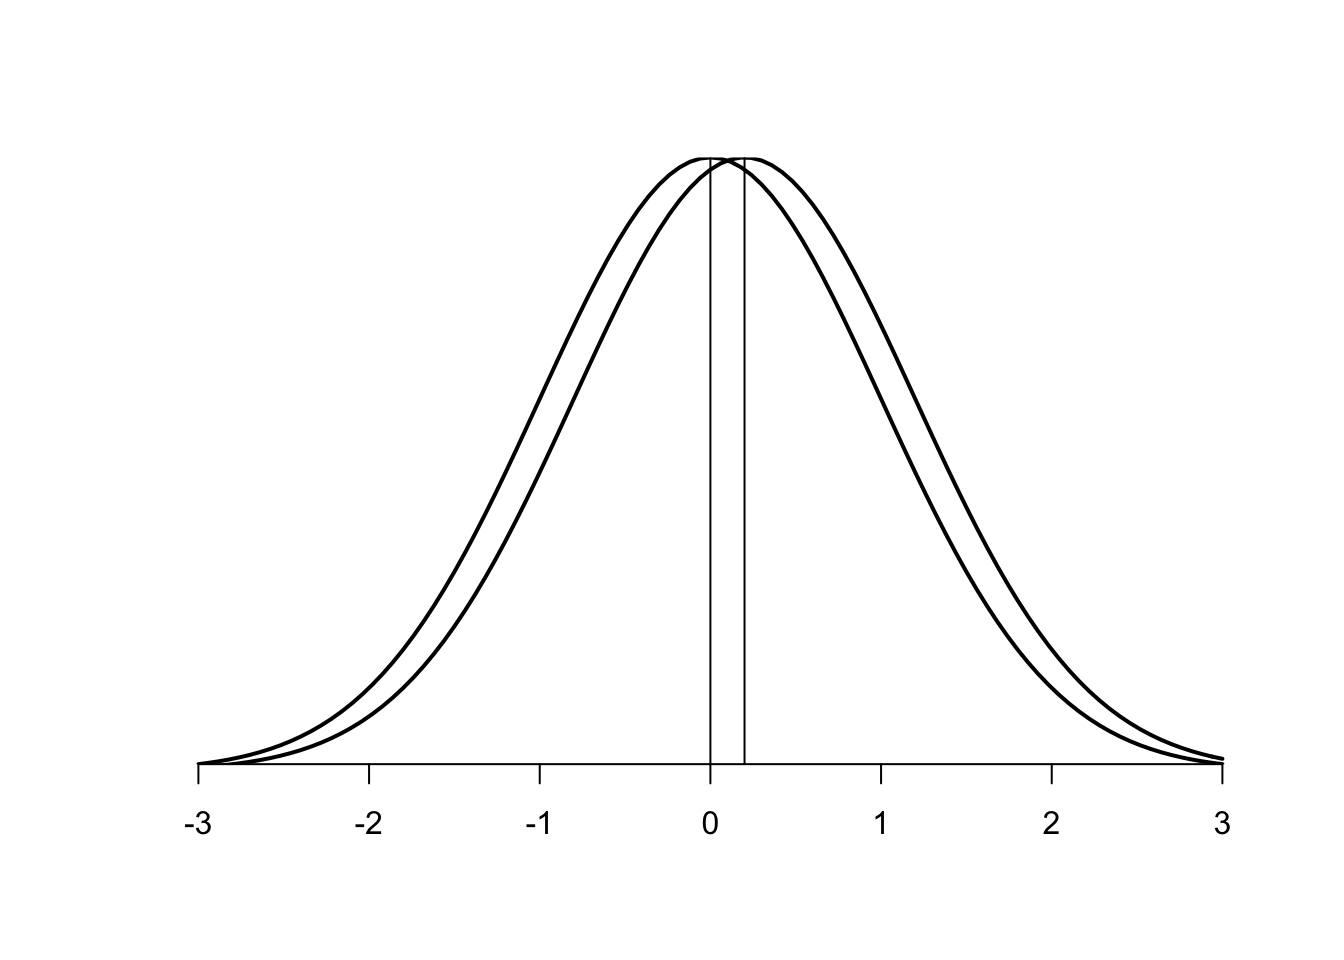
\includegraphics{Data-Analysis-for-Psychology_files/figure-latex/cohend_distribution_chap07-1.pdf}

\paragraph{その他の効果量}

Cohen's
d以外にも,効果量の指標が提案されている。詳しくは,大久保・岡田(2012)「伝えるための心理統計学」の第3章を参照。

\subsection{検定力}

\subsubsection{第Ⅱ種の過誤}\label{-1}

\begin{itemize}
\item
  第Ⅱ種の過誤(β)とは,「帰無仮説が偽なのに,帰無仮説を採択してしまう」誤りのことであった。\\
\item
  検定力とは,正しい判断の確率,つまり「帰無仮説が偽であるときに,正しく帰無仮説を棄却する確率」であった。\\
\item
  検定力は1 -
  βで求められる(全体の確率から第2種の過誤を犯す確率を引いたもの)
\item
  検定力は有意水準(α=0.05)と違って特に基準が定まっているわけではないが,.80を水準として設定するのが良いとされている(5回に1回の誤りは許す:β=0.2)。
\item
  後述するように,統計的検定の検定力は標本数にも依存する。標本数が大きければ検定力は上がる(わずかな差でも''有意差''として検出してしまう)。標本数が少なければ検定力は下がる。
\end{itemize}

\subsection{有意水準,効果量,検定力,標本数の関係}

\begin{itemize}
\tightlist
\item
  有意水準,効果量,検定力,標本数はそれぞれ関わり合っている。

  \begin{itemize}
  \tightlist
  \item
    標本数が増えれば有意な結果が出やすくなるというのは既に見たとおり。
  \item
    いたずらに標本数を増やせば意味のない差も検出されてしまう。無駄な労力にもなる。
  \end{itemize}
\item
  これら4つのパラメータのうち,研究者が左右できるのは「標本数」だけである。

  \begin{itemize}
  \tightlist
  \item
    効果量は研究で明らかにしたいものそのもの。測定しなければわからない(事前に知ることはできない。先行研究からこれくらいだろうと予想することはできる)。
  \item
    研究の前にあらかじめ「有意水準」,「効果量(の予想)」,「検定力」を決めておけば,取るべき標本数が定まる(事前の検定力分析)。
  \item
    データの取得後に,「有意水準」,「効果量」,「標本数」から,そのデータに対する「検定力」を調べることができる(事後の検定力分析)。
  \end{itemize}
\item
  Rでは,pwrパッケージにある関数を用いて検定力の分析をすることができる。
\end{itemize}

\begin{Shaded}
\begin{Highlighting}[]
\CommentTok{#事前の検定力分析(標本数の設計)}
\CommentTok{#2群間の差をt検定で検定する場合}
\CommentTok{#各群の標本数(n),効果量(d: Cohen's d),有意水準(sig.level),検定力(power)のどれか3つを入れると,入れなかったものの結果が出力される。}
\NormalTok{pwr}\OperatorTok{::}\KeywordTok{pwr.t.test}\NormalTok{(}\DataTypeTok{d=}\FloatTok{0.5}\NormalTok{, }\DataTypeTok{power=}\FloatTok{0.8}\NormalTok{, }\DataTypeTok{sig.level=}\FloatTok{0.05}\NormalTok{, }\DataTypeTok{n=}\OtherTok{NULL}\NormalTok{)}
\end{Highlighting}
\end{Shaded}

\begin{verbatim}
## 
##      Two-sample t test power calculation 
## 
##               n = 63.76561
##               d = 0.5
##       sig.level = 0.05
##           power = 0.8
##     alternative = two.sided
## 
## NOTE: n is number in *each* group
\end{verbatim}

\begin{Shaded}
\begin{Highlighting}[]
\CommentTok{#事後の検定力分析}
\CommentTok{#2群それぞれの標本数(n1, n2),効果量(d), 有意水準(sig.level)を入れると,検定力が求められる。}
\NormalTok{pwr}\OperatorTok{::}\KeywordTok{pwr.t2n.test}\NormalTok{(}\DataTypeTok{n1=}\DecValTok{10}\NormalTok{, }\DataTypeTok{n2=}\DecValTok{10}\NormalTok{, }\DataTypeTok{d=}\FloatTok{0.8}\NormalTok{, }\DataTypeTok{sig.level=}\FloatTok{0.05}\NormalTok{, }\DataTypeTok{power=}\OtherTok{NULL}\NormalTok{)}
\end{Highlighting}
\end{Shaded}

\begin{verbatim}
## 
##      t test power calculation 
## 
##              n1 = 10
##              n2 = 10
##               d = 0.8
##       sig.level = 0.05
##           power = 0.3950692
##     alternative = two.sided
\end{verbatim}

\subsection{信頼区間}

\begin{itemize}
\item
  95\%信頼区間(95\% confidence
  interval)は,95\%の確率で母数が含まれる範囲のことを言う。
\item
  例えば,母集団からランダムに20個の標本を抽出し,平均を求める。
\end{itemize}

\begin{Shaded}
\begin{Highlighting}[]
\KeywordTok{set.seed}\NormalTok{(}\DecValTok{1234}\NormalTok{)}
\NormalTok{sample_data2 =}\StringTok{ }\KeywordTok{rnorm}\NormalTok{(}\DataTypeTok{n=}\DecValTok{20}\NormalTok{, }\DataTypeTok{mean=}\DecValTok{0}\NormalTok{, }\DataTypeTok{sd=}\DecValTok{1}\NormalTok{)}
\NormalTok{sample_data2}
\end{Highlighting}
\end{Shaded}

\begin{verbatim}
##  [1] -1.20706575  0.27742924  1.08444118 -2.34569770  0.42912469
##  [6]  0.50605589 -0.57473996 -0.54663186 -0.56445200 -0.89003783
## [11] -0.47719270 -0.99838644 -0.77625389  0.06445882  0.95949406
## [16] -0.11028549 -0.51100951 -0.91119542 -0.83717168  2.41583518
\end{verbatim}

\begin{Shaded}
\begin{Highlighting}[]
\KeywordTok{mean}\NormalTok{(sample_data2)}
\end{Highlighting}
\end{Shaded}

\begin{verbatim}
## [1] -0.2506641
\end{verbatim}

平均は-0.25であった。この20個のデータから,母集団の平均を推定する。

\begin{itemize}
\tightlist
\item
  標本から得られた値をもとに母集団のパラメータを評価する手続きは,推定と呼ばれる。\\
\item
  もちろん,正確な母集団の平均値を当てることは難しい。そこで,母集団の平均値が入るだろうと予測される範囲を推定する。これが,信頼区間である。
\end{itemize}

\subsubsection{信頼区間の求め方}

例えば平均値の信頼区間は以下のように求める。

\[
CI = \bar{X} + ME\\
ME =  SE \times \pm t_{95\%} 
\]

\begin{itemize}
\tightlist
\item
  MEは誤差範囲(margin of
  errors)である。つまり,標本から得られた値について正及び負の方向に誤差を加えた値が信頼区間の上限及び下限値となる。
\item
  誤差範囲には標準誤差(SE)を用いる。
\end{itemize}

データが正規分布に従うのならば,誤差範囲はt分布を使って求めるのが一般的。\(t_{95\%}\)は,t分布の95%点に対応する(t分布の下位または上位2.5\%に対応するtの値)。

\begin{Shaded}
\begin{Highlighting}[]
\CommentTok{#conf.levelの値を変えれば,信頼区間の範囲を任意で設定できる(デフォルトで0.95)}
\KeywordTok{t.test}\NormalTok{(sample_data2, }\DataTypeTok{conf.level =} \FloatTok{0.95}\NormalTok{)}
\end{Highlighting}
\end{Shaded}

\begin{verbatim}
## 
##  One Sample t-test
## 
## data:  sample_data2
## t = -1.1057, df = 19, p-value = 0.2826
## alternative hypothesis: true mean is not equal to 0
## 95 percent confidence interval:
##  -0.7251406  0.2238125
## sample estimates:
##  mean of x 
## -0.2506641
\end{verbatim}

平均値の信頼区間ならば,Rではt.test関数でも求めることができる。

\subsubsection{信頼区間と統計的帰無仮説検定の関係}

\begin{itemize}
\tightlist
\item
  信頼区間は統計的帰無仮説検定と表裏一体である。\\
\item
  例えば「母集団の平均値は0ではない」という帰無仮説を評価する。すなわち,母集団の平均値の95%信頼区間にゼロが含まれていなければ,帰無仮説は棄却されることになる。\\
\item
  標本数を増やせば(標準)誤差が小さくなるので,信頼区間の範囲も狭くなる。
\end{itemize}

\subsubsection{平均値以外の信頼区間の求め方}

\begin{itemize}
\tightlist
\item
  割合について求める場合は,Rならばbinom.test関数で求められる。
\end{itemize}

\begin{Shaded}
\begin{Highlighting}[]
\CommentTok{#100人中,30人がある意見に賛成した場合。母集団の賛成率の信頼区間は?}
\CommentTok{#conf.levelの値を変えれば,信頼区間の範囲を任意で設定できる(デフォルトで0.95)}
\KeywordTok{binom.test}\NormalTok{(}\DataTypeTok{x=}\DecValTok{30}\NormalTok{, }\DataTypeTok{n=}\DecValTok{100}\NormalTok{, }\DataTypeTok{conf.level =} \FloatTok{0.95}\NormalTok{)}
\end{Highlighting}
\end{Shaded}

\begin{verbatim}
## 
##  Exact binomial test
## 
## data:  30 and 100
## number of successes = 30, number of trials = 100, p-value =
## 7.85e-05
## alternative hypothesis: true probability of success is not equal to 0.5
## 95 percent confidence interval:
##  0.2124064 0.3998147
## sample estimates:
## probability of success 
##                    0.3
\end{verbatim}

\begin{itemize}
\item
  もちろん,他の統計量についても,同じく信頼区間を評価することは可能。相関係数,回帰係数,効果量などについても求められる(詳しくは,大久保・岡田,
  2012)。
\item
  信頼区間を評価することで,その推定値の正確さや範囲を評価することができる。\\
\item
  信頼区間を報告するときは一般的に,CI = {[}-0.56,
  0.36{]}といったように表現する。
\item
  最近の心理学においても,信頼区間の報告が求められるようになっている。グラフのエラーバーの範囲にも信頼区間を載せることも多い(95\%水準で有意差があるのかがわかりやすくなる)
\end{itemize}

\subsection{参考文献}\label{-1}

大久保街亜・岡田謙介 (2012). 伝えるための心理統計 勁草書房

\subsection{練習問題}\label{-7}

\subsubsection{問1}\label{-15}

\begin{itemize}
\tightlist
\item
  二群間で平均値をt検定で比較する場合,効果量が小さい,中くらい,大きいとき(それぞれ,d=0.2,
  d=0.5,
  d=0.8),それぞれで一群あたり何名程度の参加者を取ればよいか?有意水準を0.05,
  検定力を0.8とした上で求めよ。

  \begin{itemize}
  \tightlist
  \item
    ヒント:Rのpwrパッケージのpwr.t.test関数を使えば求まる。
  \end{itemize}
\end{itemize}

\subsubsection{問2}\label{-16}

\paragraph{小問1}\label{1}

\begin{itemize}
\tightlist
\item
  以下のプログラムを読み込む。\\
\item
  あるサプリメントにダイエットの効果があるかを検討するために,10名を対象に実験を行った。それぞれの参加者にサプリメントを投与する前(before)と投与した後(after)で体重を測定した(架空のデータである)。
\end{itemize}

\begin{Shaded}
\begin{Highlighting}[]
\NormalTok{before =}\StringTok{ }\KeywordTok{c}\NormalTok{(}\FloatTok{37.93}\NormalTok{, }\FloatTok{52.77}\NormalTok{, }\FloatTok{60.84}\NormalTok{, }\FloatTok{26.54}\NormalTok{, }\FloatTok{54.29}\NormalTok{, }\FloatTok{55.06}\NormalTok{, }\FloatTok{44.25}\NormalTok{, }\FloatTok{44.53}\NormalTok{, }\FloatTok{44.36}\NormalTok{, }\FloatTok{41.1}\NormalTok{)}
\NormalTok{after =}\StringTok{ }\KeywordTok{c}\NormalTok{(}\FloatTok{57.84}\NormalTok{, }\FloatTok{50.02}\NormalTok{, }\FloatTok{53.36}\NormalTok{, }\FloatTok{65.97}\NormalTok{, }\FloatTok{79.39}\NormalTok{, }\FloatTok{63.35}\NormalTok{, }\FloatTok{57.33}\NormalTok{, }\FloatTok{51.33}\NormalTok{, }\FloatTok{52.44}\NormalTok{, }\FloatTok{101.24}\NormalTok{)}
\NormalTok{Value =}\StringTok{ }\KeywordTok{c}\NormalTok{(before, after)}
\NormalTok{Treatment =}\StringTok{ }\KeywordTok{c}\NormalTok{(}\KeywordTok{rep}\NormalTok{(}\StringTok{"before"}\NormalTok{, }\DecValTok{10}\NormalTok{), }\KeywordTok{rep}\NormalTok{(}\StringTok{"after"}\NormalTok{, }\DecValTok{10}\NormalTok{))}
\NormalTok{Subject =}\StringTok{ }\KeywordTok{c}\NormalTok{(}\KeywordTok{c}\NormalTok{(}\DecValTok{1}\OperatorTok{:}\DecValTok{10}\NormalTok{), }\KeywordTok{c}\NormalTok{(}\DecValTok{1}\OperatorTok{:}\DecValTok{10}\NormalTok{))}
\NormalTok{sample_}\DecValTok{1}\NormalTok{ =}\StringTok{ }\KeywordTok{data.frame}\NormalTok{(}\DataTypeTok{Subject =}\NormalTok{ Subject, }\DataTypeTok{Treatment =}\NormalTok{ Treatment, }\DataTypeTok{Value =}\NormalTok{ Value)}
\NormalTok{sample_}\DecValTok{1}
\end{Highlighting}
\end{Shaded}

\begin{verbatim}
##    Subject Treatment  Value
## 1        1    before  37.93
## 2        2    before  52.77
## 3        3    before  60.84
## 4        4    before  26.54
## 5        5    before  54.29
## 6        6    before  55.06
## 7        7    before  44.25
## 8        8    before  44.53
## 9        9    before  44.36
## 10      10    before  41.10
## 11       1     after  57.84
## 12       2     after  50.02
## 13       3     after  53.36
## 14       4     after  65.97
## 15       5     after  79.39
## 16       6     after  63.35
## 17       7     after  57.33
## 18       8     after  51.33
## 19       9     after  52.44
## 20      10     after 101.24
\end{verbatim}

\begin{itemize}
\tightlist
\item
  対応のあるt検定で投与前と投与後の体重の比較をし,帰無仮説が棄却されるかについて結論を述べよ。

  \begin{itemize}
  \tightlist
  \item
    ヒント:対応のあるt検定のやりかたについては,第6回の資料を参照。
  \end{itemize}
\end{itemize}

\paragraph{小問2}

\begin{itemize}
\tightlist
\item
  以下のデータは,小問1のデータを横に並べ替えたものである。参加者1人につき1行,投与前(before)と投与後(after)も数値が入力されている。
\end{itemize}

\begin{Shaded}
\begin{Highlighting}[]
\NormalTok{sample_}\DecValTok{2}\NormalTok{ =}\StringTok{ }\KeywordTok{data.frame}\NormalTok{(}\DataTypeTok{Subject =} \KeywordTok{c}\NormalTok{(}\DecValTok{1}\OperatorTok{:}\DecValTok{10}\NormalTok{), }\DataTypeTok{before =}\NormalTok{ before, }\DataTypeTok{after =}\NormalTok{ after)}
\NormalTok{sample_}\DecValTok{2}
\end{Highlighting}
\end{Shaded}

\begin{verbatim}
##    Subject before  after
## 1        1  37.93  57.84
## 2        2  52.77  50.02
## 3        3  60.84  53.36
## 4        4  26.54  65.97
## 5        5  54.29  79.39
## 6        6  55.06  63.35
## 7        7  44.25  57.33
## 8        8  44.53  51.33
## 9        9  44.36  52.44
## 10      10  41.10 101.24
\end{verbatim}

\begin{itemize}
\tightlist
\item
  投与前と投与後の体重の差を求めて,体重の差の95\%信頼区間を求めよ。

  \begin{itemize}
  \tightlist
  \item
    ヒント:投与前と投与後の差の変数を作る。つまり,beforeからafterを引き(逆でも可),diffという新しい変数を作る。新しく作った変数をt.test()に入れれば95\%信頼区間が求まる。
  \end{itemize}
\end{itemize}

\section{回帰分析}

\begin{itemize}
\tightlist
\item
  回帰分析の基礎について学ぶ。

  \begin{itemize}
  \tightlist
  \item
    回帰分析
  \item
    最小二乗法
  \item
    重回帰分析
  \end{itemize}
\end{itemize}

\subsection{準備}\label{-5}

\begin{Shaded}
\begin{Highlighting}[]
\KeywordTok{install.packages}\NormalTok{(}\StringTok{"tidyverse"}\NormalTok{)}
\KeywordTok{install.packages}\NormalTok{(}\StringTok{"car"}\NormalTok{)}
\KeywordTok{library}\NormalTok{(tidyverse)}
\KeywordTok{library}\NormalTok{(car)}
\end{Highlighting}
\end{Shaded}

\subsection{回帰分析}\label{-1}

以下のプログラムを読み込み,サンプルデータを作る。

\begin{Shaded}
\begin{Highlighting}[]
\CommentTok{#架空のデータを作る}
\KeywordTok{set.seed}\NormalTok{(}\DecValTok{1234}\NormalTok{)}
\NormalTok{N =}\StringTok{ }\DecValTok{100}
\NormalTok{a =}\StringTok{ }\DecValTok{10}
\NormalTok{b1 =}\StringTok{ }\DecValTok{3}
\NormalTok{b2 =}\StringTok{ }\FloatTok{0.5}
\NormalTok{x1 =}\StringTok{ }\KeywordTok{rnorm}\NormalTok{(}\DataTypeTok{n =}\NormalTok{ N)}
\NormalTok{x2 =}\StringTok{ }\KeywordTok{rnorm}\NormalTok{(}\DataTypeTok{n =}\NormalTok{ N)}
\NormalTok{e =}\StringTok{ }\KeywordTok{rnorm}\NormalTok{(}\DataTypeTok{n =}\NormalTok{ N, }\DataTypeTok{sd =} \DecValTok{5}\NormalTok{)}
\NormalTok{y =}\StringTok{ }\NormalTok{b1}\OperatorTok{*}\NormalTok{x1 }\OperatorTok{+}\StringTok{ }\NormalTok{b2}\OperatorTok{*}\NormalTok{x2 }\OperatorTok{+}\StringTok{ }\NormalTok{a }\OperatorTok{+}\StringTok{ }\NormalTok{e}
\NormalTok{sample_data =}\StringTok{ }\KeywordTok{data.frame}\NormalTok{(}\DataTypeTok{x1 =}\NormalTok{ x1, }\DataTypeTok{x2 =}\NormalTok{ x2, }\DataTypeTok{y=}\NormalTok{ y)}

\KeywordTok{head}\NormalTok{(sample_data) }\CommentTok{#サンプルデータの上数行を表示}
\end{Highlighting}
\end{Shaded}

\begin{verbatim}
##           x1          x2         y
## 1 -1.2070657  0.41452353  9.012199
## 2  0.2774292 -0.47471847 14.078772
## 3  1.0844412  0.06599349 14.213890
## 4 -2.3456977 -0.50247778  6.215336
## 5  0.4291247 -0.82599859 12.432780
## 6  0.5060559  0.16698928 15.403974
\end{verbatim}

\begin{Shaded}
\begin{Highlighting}[]
\KeywordTok{qplot}\NormalTok{(}\DataTypeTok{data=}\NormalTok{sample_data, x1, y) }\CommentTok{#x1とyの散布図を示す}
\end{Highlighting}
\end{Shaded}

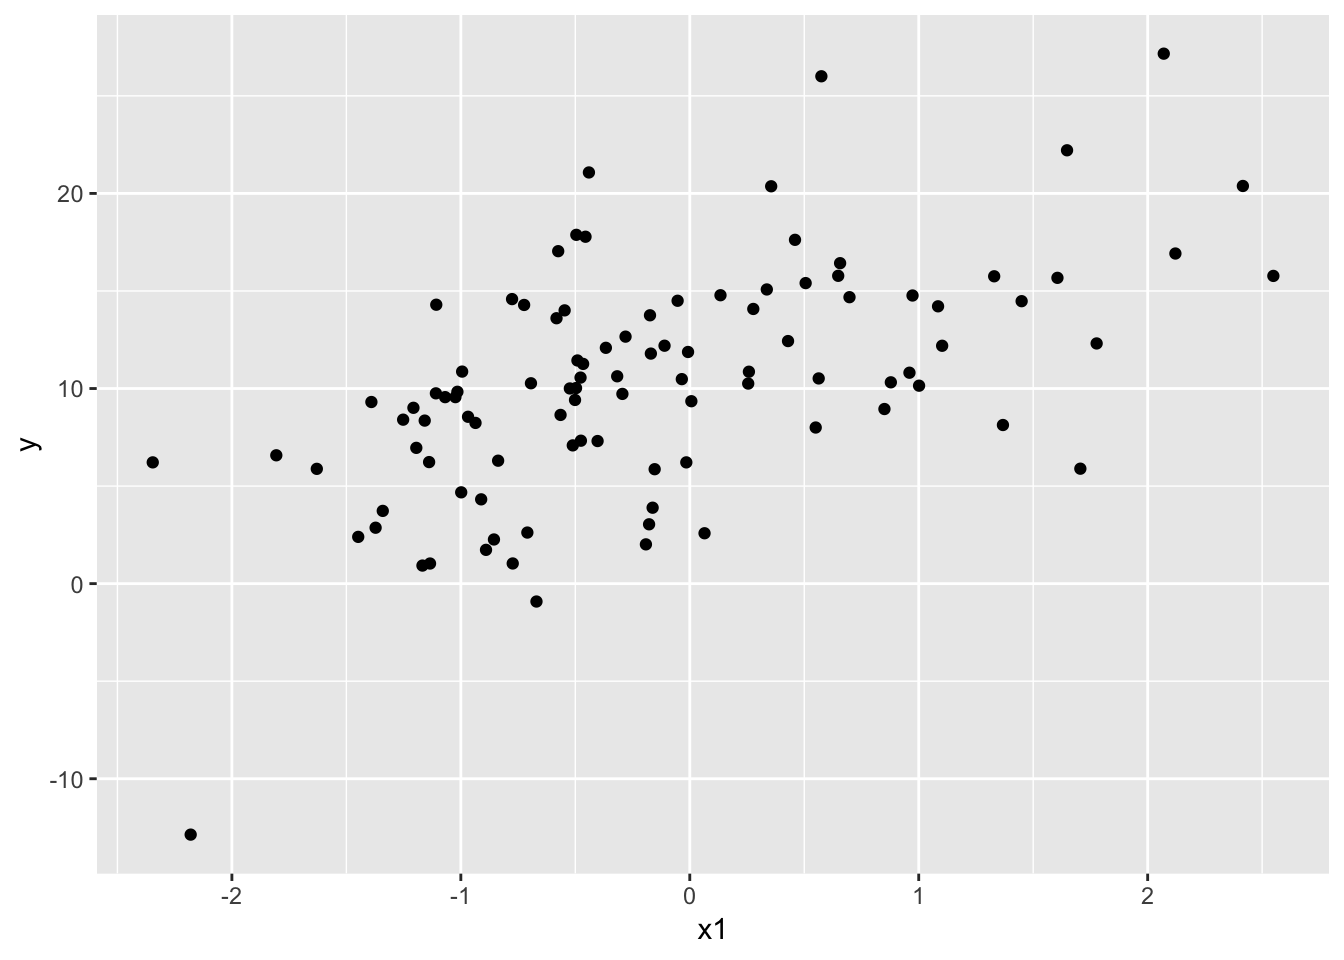
\includegraphics{Data-Analysis-for-Psychology_files/figure-latex/read_regression_data_chap08-1.pdf}

\begin{itemize}
\item
  以下のことが知りたい。

  \begin{itemize}
  \tightlist
  \item
    新たに測定を行ったとき,x1 = 0.1 の値が得られた。この値から,y
    がどのような値になるのか?(新たなデータから,yを予測する)
  \item
    x1 が 1増えたら,y
    がどれくらい増えるのか?(x1の効果の強さを知りたい)
  \end{itemize}
\end{itemize}

回帰分析(regresion
analysis)は,「データの予測」と「効果の測定」を目的として行う。

\begin{itemize}
\tightlist
\item
  回帰分析とは,以下の式により独立変数の値から従属変数の値を予測する解析である。以下のような式は,「回帰式」あるいは「線形予測子」と呼ばれる。
\end{itemize}

\[
\hat{y} = bx+a
\]

xを独立変数,yを従属変数とする。\(\hat{y}\)は,yの予測値とする。傾きbと切片aをデータから求める。
実測値であるyと予測値である\(\hat{y}\)の差が最も小さくなるときの,bとaを求める。

\begin{itemize}
\tightlist
\item
  回帰分析はシンプルな直線の式から結果を予測する解析である。
\item
  切片aは,独立変数xがゼロのときの従属変数の予測値を表現している。\\
\item
  傾きは,回帰係数(regression coefficient)と呼ばれる。\\
\item
  回帰係数は独立変数が従属変数にもたらす効果の強さを意味する。つまり,効果量の一種ともいえる。
\end{itemize}

なお,回帰分析において独立変数を「\textbf{説明変数}」,従属変数を「\textbf{目的変数},\textbf{応答変数},ないしは\textbf{被説明変数}」という場合もある。

\subsubsection{回帰分析の結果の解釈}

回帰分析をする場合,Rではlm()関数を使う。

\begin{Shaded}
\begin{Highlighting}[]
\NormalTok{result =}\StringTok{ }\KeywordTok{lm}\NormalTok{(}\DataTypeTok{data =}\NormalTok{ sample_data, y }\OperatorTok{~}\StringTok{ }\NormalTok{x1) }\CommentTok{#結果を別の変数で保存しておき,summary()関数で詳細な結果を出すことができる}
\KeywordTok{summary}\NormalTok{(result)}
\end{Highlighting}
\end{Shaded}

\begin{verbatim}
## 
## Call:
## lm(formula = y ~ x1, data = sample_data)
## 
## Residuals:
##      Min       1Q   Median       3Q      Max 
## -16.3526  -3.3001   0.5401   2.6685  13.2098 
## 
## Coefficients:
##             Estimate Std. Error t value Pr(>|t|)    
## (Intercept)  10.8529     0.4945   21.95  < 2e-16 ***
## x1            3.3780     0.4889    6.91 4.94e-10 ***
## ---
## Signif. codes:  0 '***' 0.001 '**' 0.01 '*' 0.05 '.' 0.1 ' ' 1
## 
## Residual standard error: 4.886 on 98 degrees of freedom
## Multiple R-squared:  0.3276, Adjusted R-squared:  0.3207 
## F-statistic: 47.74 on 1 and 98 DF,  p-value: 4.935e-10
\end{verbatim}

\begin{itemize}
\tightlist
\item
  係数(Coefficients)の結果を見る。

  \begin{itemize}
  \tightlist
  \item
    Interceptは切片を意味する。x1が独立変数の傾きを意味する。\\
  \item
    Estimateが推定された切片または傾きの値である。\\
  \item
    Std.Errorは推定された係数の標準誤差である。\\
  \item
    t
    value及びPrは係数の有意性検定の結果を示している(それぞれt値,p値)。ここでは,「係数がゼロである」という帰無仮説を検定している。p値が極端に低い場合は,「求めた係数の値は有意にゼロから乖離している」と結論付けることができる。
  \end{itemize}
\item
  傾きが意味することは,独立変数が1単位増えたら従属変数がどう変化するかということである。

  \begin{itemize}
  \tightlist
  \item
    係数がプラスならば,係数の値が増えると従属変数の値が増える関係にあることを意味する。
  \item
    係数がマイナスならば,係数が値が増えると従属変数が減る関係にあることを意味する。
  \end{itemize}
\item
  さっきの散布図に回帰分析から求めた回帰直線を引いてみよう。
\end{itemize}

\begin{Shaded}
\begin{Highlighting}[]
\NormalTok{p =}\StringTok{ }\KeywordTok{qplot}\NormalTok{(}\DataTypeTok{data =}\NormalTok{ sample_data, x1, y)}
\NormalTok{p =}\StringTok{ }\NormalTok{p }\OperatorTok{+}\StringTok{ }\KeywordTok{stat_smooth}\NormalTok{(}\DataTypeTok{method =} \StringTok{"lm"}\NormalTok{, }\DataTypeTok{se =} \OtherTok{FALSE}\NormalTok{)}
\NormalTok{p}
\end{Highlighting}
\end{Shaded}

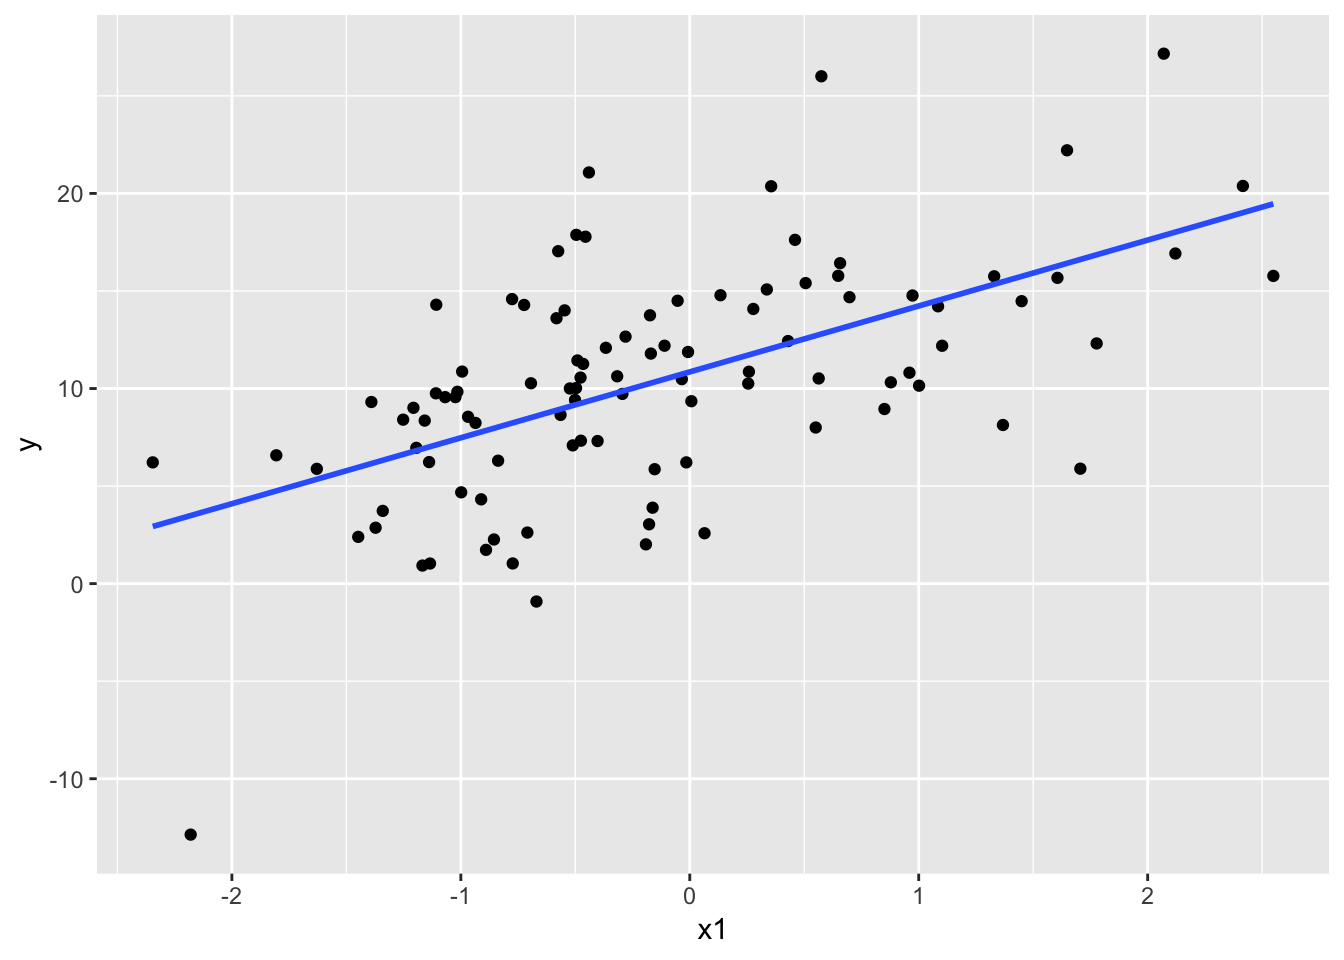
\includegraphics{Data-Analysis-for-Psychology_files/figure-latex/read_regression_plot_chap08-1.pdf}

概ねデータに重なるかたちで直線が引かれている。

\begin{itemize}
\tightlist
\item
  他にも出力に「Multiple
  R-Squared」とあるが,これは「決定係数」と呼ばれるもので,データの全ての分散のうち,今回の回帰分析によって説明できている割合を意味する。0から1の範囲を取り,1に近いほど今回の回帰分析の結果がデータを良く説明できていることを意味する。
\end{itemize}

\[
R^2 = \frac{\sum^n_{i=1}(\hat{y}_i-\bar{y})^2}{\sum^n_{i=1}(y_i-\bar{y})^2}
\]
\(y\)は実測値,\(\bar{y}\)は実測値yの平均値,\(\hat{y}\)は回帰分析で求めたyの予測値を意味する。

\subsubsection{最小二乗法}

では,回帰分析では傾きと切片の値をどう求めているのだろうか?

実測値と予測値との差は残差(Residual
value)と呼ばれる。残差が最も小さくなるときの傾き及び切片を,yを予測する上で最適な傾き及び切片の値として採用する(残差が最小となるときの式が,データをうまく説明できていると解釈できる)。
このような回帰式の切片及び傾きの求め方を,「最小二乗法」という。

\begin{itemize}
\tightlist
\item
  ある条件のもとで結果を最小あるいは最大にする手法のことを,数学では最適化と呼ぶ。最小二乗法とは最適化手法の一種である。
\item
  当然ながら手計算では困難である。普通はコンピュータを使って計算する。Rには最適化を行うための関数optim()が用意されている。
\item
  あくまで参考までに,最小二乗法をoptim関数で行ったプログラムを以下に示す。
\end{itemize}

\begin{Shaded}
\begin{Highlighting}[]
\NormalTok{y =}\StringTok{ }\NormalTok{sample_data}\OperatorTok{$}\NormalTok{y}
\NormalTok{x1 =}\StringTok{ }\NormalTok{sample_data}\OperatorTok{$}\NormalTok{x1}

\NormalTok{residual =}\StringTok{ }\ControlFlowTok{function}\NormalTok{(para)\{}
\NormalTok{    b =}\StringTok{ }\NormalTok{para[}\DecValTok{1}\NormalTok{]}
\NormalTok{    a =}\StringTok{ }\NormalTok{para[}\DecValTok{2}\NormalTok{]}
\NormalTok{    hat_y =}\StringTok{ }\NormalTok{b}\OperatorTok{*}\NormalTok{x1 }\OperatorTok{+}\StringTok{ }\NormalTok{a }\CommentTok{#x1とパラメータa, bから,予測値hat_yを計算する}
    \KeywordTok{sum}\NormalTok{((y }\OperatorTok{-}\StringTok{ }\NormalTok{hat_y)}\OperatorTok{^}\DecValTok{2}\NormalTok{) }\CommentTok{#予測値と実測値との差の二乗の合計値を求めたものをresidualという変数で保存}
\NormalTok{\}}


\KeywordTok{optim}\NormalTok{(}\DataTypeTok{par =} \KeywordTok{c}\NormalTok{(}\DecValTok{1}\NormalTok{, }\DecValTok{1}\NormalTok{), residual) }\CommentTok{#特に何も指定しなければ,residualという変数を最小化せよという命令となる(par=c(1, 1)は,bとaを計算するときの初期値を1, 1にせよという命令。あまり深く考えなくて良い)。出力結果の「par」に,傾き(b)と切片(a)の推定結果が出る。lm()関数を使って計算した値と近似しているはず。}
\end{Highlighting}
\end{Shaded}

\begin{verbatim}
## $par
## [1]  3.379037 10.852593
## 
## $value
## [1] 2339.32
## 
## $counts
## function gradient 
##       67       NA 
## 
## $convergence
## [1] 0
## 
## $message
## NULL
\end{verbatim}

最小二乗法以外にも,「\textbf{最尤法}(さいゆうほう)」という最適化手法でも同じ回帰係数を求めることができる。最尤法については,一般化線形モデルの回で説明する。

\subsection{重回帰分析}

独立変数が複数の場合の回帰分析は,重回帰分析(multivariant regression
analysis)と呼ばれる。\\
独立変数が一つの場合は,単回帰分析と呼んで区別することもある。

例えば,独立変数が2つの場合の回帰式は以下のようになる。

\[
\hat{y} = b_{1}x_{1}+b_{2}x_{2} + a
\]

\begin{Shaded}
\begin{Highlighting}[]
\NormalTok{result_}\DecValTok{2}\NormalTok{ =}\StringTok{ }\KeywordTok{lm}\NormalTok{(}\DataTypeTok{data=}\NormalTok{sample_data, y }\OperatorTok{~}\StringTok{ }\NormalTok{x1 }\OperatorTok{+}\StringTok{ }\NormalTok{x2)}
\KeywordTok{summary}\NormalTok{(result_}\DecValTok{2}\NormalTok{)}
\end{Highlighting}
\end{Shaded}

\begin{verbatim}
## 
## Call:
## lm(formula = y ~ x1 + x2, data = sample_data)
## 
## Residuals:
##     Min      1Q  Median      3Q     Max 
## -15.966  -3.367   0.530   2.912  13.825 
## 
## Coefficients:
##             Estimate Std. Error t value Pr(>|t|)    
## (Intercept)  10.8179     0.4874  22.196  < 2e-16 ***
## x1            3.4026     0.4816   7.065 2.46e-10 ***
## x2            0.9416     0.4687   2.009   0.0473 *  
## ---
## Signif. codes:  0 '***' 0.001 '**' 0.01 '*' 0.05 '.' 0.1 ' ' 1
## 
## Residual standard error: 4.812 on 97 degrees of freedom
## Multiple R-squared:  0.3544, Adjusted R-squared:  0.3411 
## F-statistic: 26.63 on 2 and 97 DF,  p-value: 6.049e-10
\end{verbatim}

例えば変数 X1 の回帰係数は,他の独立変数の効果が同じとした場合に X1
が1単位増えた時の y の変化量を意味している。
このように他の変数の影響を統制(control)した上で独立変数の効果を検討することができるのが,回帰分析のメリットの一つである。

\subsubsection{多重共線性}

\begin{itemize}
\item
  独立変数同士が強く相関していると,回帰分析の結果は信用できない恐れがある。このような問題は「多重共線性(multicollinearity)」と呼ばれる。例えば,\(x_{1}\)と\(x_{2}\)が相関している,つまりほぼ\(x_{1}=x_{2}\)と言える場合,傾きの値もほぼ\(b_{1}=b_{2}\)となる。この場合,傾きの組み合わせが複数ありえるため(\(b_{1}=1, b_{2}=2\)や\(b_{1}=2, b_{2}=1\)),パラメータの値を推定することが出来ない。
\item
  独立変数同士の相関が0.8を超えている場合は,多重共線性を疑った方が良い。\\
\item
  多重共線性を疑う基準として,VIF(Variance inflation
  factor)と呼ばれる指標もある。VIFが10を超えていたら,多重共線性を疑った方が良いとされている。
\end{itemize}

\[
VIF = \frac{1}{1-R^2}
\]
上の式の\(R^2\)は,ある独立変数を従属変数としたときの他の独立変数による重回帰分析での決定係数を意味する。

\begin{itemize}
\tightlist
\item
  carパッケージのvif()関数を使うと,VIFを計算してくれる。
\end{itemize}

\begin{Shaded}
\begin{Highlighting}[]
\NormalTok{car}\OperatorTok{::}\KeywordTok{vif}\NormalTok{(result_}\DecValTok{2}\NormalTok{) }\CommentTok{#lm()関数で計算した回帰分析の結果を入れれば良い。}
\end{Highlighting}
\end{Shaded}

\begin{verbatim}
##       x1       x2 
## 1.000645 1.000645
\end{verbatim}

\subsubsection{決定係数}

\begin{itemize}
\tightlist
\item
  先に説明したように,決定係数は回帰分析によって説明されるデータの分散の割合,すなわち「回帰分析の精度の良さ」を示す指標として認識されている。\\
\item
  しかし,決定係数は基本的に独立変数を多く入れれば大きい値を取る傾向にある(意味のない変数を入れたとしても,データの分散を多少は説明できるようになる)。\\
\item
  この問題を解消するために,決定係数とは別に「情報量基準」という指標が用いられている。詳しくは「一般化線形モデル」の回で説明する。
\end{itemize}

\subsection{ダミー変数(独立変数が質的変数の場合)}

\begin{itemize}
\tightlist
\item
  上の例は独立変数が量的変数の場合を用いたが,質的変数(性別,学生か否かなど)の場合でも可能である。解析の際には,変数を0か1の変数に変換する必要がある。ダミー変数(dummy
  variable)と呼ばれる。
\end{itemize}

\begin{Shaded}
\begin{Highlighting}[]
\CommentTok{#サンプルデータの作成}
\KeywordTok{set.seed}\NormalTok{(}\DecValTok{1234}\NormalTok{)}
\NormalTok{y =}\StringTok{ }\KeywordTok{rnorm}\NormalTok{(}\DecValTok{100}\NormalTok{)}
\NormalTok{x =}\StringTok{ }\KeywordTok{round}\NormalTok{(}\KeywordTok{runif}\NormalTok{(}\DecValTok{100}\NormalTok{),}\DecValTok{0}\NormalTok{)}
\NormalTok{sampledata_}\DecValTok{2}\NormalTok{ =}\StringTok{ }\KeywordTok{data.frame}\NormalTok{(}\DataTypeTok{y =}\NormalTok{ y,}\DataTypeTok{x =}\NormalTok{ x)}

\KeywordTok{head}\NormalTok{(sampledata_}\DecValTok{2}\NormalTok{) }\CommentTok{#sampledata_2の上数行だけを表示する。}
\end{Highlighting}
\end{Shaded}

\begin{verbatim}
##            y x
## 1 -1.2070657 1
## 2  0.2774292 1
## 3  1.0844412 0
## 4 -2.3456977 1
## 5  0.4291247 1
## 6  0.5060559 1
\end{verbatim}

\begin{Shaded}
\begin{Highlighting}[]
\NormalTok{result_}\DecValTok{3}\NormalTok{ =}\StringTok{ }\KeywordTok{lm}\NormalTok{(}\DataTypeTok{data =}\NormalTok{ sampledata_}\DecValTok{2}\NormalTok{, y }\OperatorTok{~}\StringTok{ }\NormalTok{x)}
\KeywordTok{summary}\NormalTok{(result_}\DecValTok{3}\NormalTok{)}
\end{Highlighting}
\end{Shaded}

\begin{verbatim}
## 
## Call:
## lm(formula = y ~ x, data = sampledata_2)
## 
## Residuals:
##     Min      1Q  Median      3Q     Max 
## -2.0686 -0.7651 -0.1993  0.6510  2.6929 
## 
## Coefficients:
##             Estimate Std. Error t value Pr(>|t|)
## (Intercept) -0.02642    0.14456  -0.183    0.855
## x           -0.25066    0.20047  -1.250    0.214
## 
## Residual standard error: 1.002 on 98 degrees of freedom
## Multiple R-squared:  0.0157, Adjusted R-squared:  0.005658 
## F-statistic: 1.563 on 1 and 98 DF,  p-value: 0.2142
\end{verbatim}

独立変数が一つで二値の場合,回帰係数の有意性検定の結果は,t検定を行った場合と一致する。つまり,独立変数が二値の単回帰分析でやっていることは,2群間の平均値の差の検定と同じである。その理由は,一般化線形モデルの回で説明する。

\begin{Shaded}
\begin{Highlighting}[]
\KeywordTok{t.test}\NormalTok{(}\DataTypeTok{data =}\NormalTok{ sampledata_}\DecValTok{2}\NormalTok{, y }\OperatorTok{~}\StringTok{ }\NormalTok{x, }\DataTypeTok{paired =}\NormalTok{ F, }\DataTypeTok{var.equal =}\NormalTok{ T) }\CommentTok{#等分散を仮定した場合の検定。}
\end{Highlighting}
\end{Shaded}

\begin{verbatim}
## 
##  Two Sample t-test
## 
## data:  y by x
## t = 1.2503, df = 98, p-value = 0.2142
## alternative hypothesis: true difference in means is not equal to 0
## 95 percent confidence interval:
##  -0.1471737  0.6484883
## sample estimates:
## mean in group 0 mean in group 1 
##     -0.02641995     -0.27707724
\end{verbatim}

\subsection{練習問題}\label{-8}

問1,問2いずれも宿題とする。なお,数値は小数点第3位まで報告せよ(小数点第4位以下は四捨五入)。

\subsubsection{問1}\label{-17}

Rにはattitudeというデータが入っている。ある金融機関の30部門で従業員に行ったアンケート調査の結果である。各部署ごとに,7つの質問項目について好意的な評価をした人の割合が示されている。

\begin{itemize}
\tightlist
\item
  ちなみに,データのcomplaints, privileges, learning, raises, critical,
  advanceはそれぞれ,「従業員の不満への対応」,「特権を許さない」,「学習の機会」,「能力に応じた昇給」,「批判的すぎる」,「昇進」を意味する。
\end{itemize}

\begin{Shaded}
\begin{Highlighting}[]
\KeywordTok{head}\NormalTok{(attitude)}
\end{Highlighting}
\end{Shaded}

\begin{verbatim}
##   rating complaints privileges learning raises critical advance
## 1     43         51         30       39     61       92      45
## 2     63         64         51       54     63       73      47
## 3     71         70         68       69     76       86      48
## 4     61         63         45       47     54       84      35
## 5     81         78         56       66     71       83      47
## 6     43         55         49       44     54       49      34
\end{verbatim}

ratingを従属変数,その他の変数(complaints, privileges, learning,
raises, critical, advance)を独立変数とした重回帰分析を行い,

\paragraph{小問1}\label{-1}

それぞれの独立変数の傾きの係数及び検定の結果を報告せよ(係数の値とp値だけでよい)。

\begin{itemize}
\tightlist
\item
  ヒント:一般的に回帰係数の推定結果を論文などで報告するときは,(b=x.xxx,
  p=.xxx)とする。bは回帰係数を意味する。
\end{itemize}

\paragraph{小問2}\label{-2}

5\%水準で有意な効果を持った独立変数を挙げ,それらの独立変数の増減によって従属変数がどう変化する傾向にあるかを報告せよ。

\paragraph{小問3}\label{-3}

learningが1単位増えると,ratingはいくら変化するかを述べよ。

\subsubsection{問2}\label{-18}

以下のプログラムを読み込み,サンプルデータ dat\_q2 を作成する。

このデータには,A県とB県それぞれで10人の生徒を選んで学力テストを行った結果を示している(架空の調査である)。Prefectureが県,Value
がテストの成績を意味する。

\begin{Shaded}
\begin{Highlighting}[]
\NormalTok{A =}\StringTok{ }\KeywordTok{c}\NormalTok{(}\DecValTok{38}\NormalTok{, }\DecValTok{53}\NormalTok{, }\DecValTok{61}\NormalTok{, }\DecValTok{27}\NormalTok{, }\DecValTok{54}\NormalTok{, }\DecValTok{55}\NormalTok{, }\DecValTok{44}\NormalTok{, }\DecValTok{45}\NormalTok{, }\DecValTok{44}\NormalTok{, }\DecValTok{41}\NormalTok{)}
\NormalTok{B =}\StringTok{ }\KeywordTok{c}\NormalTok{(}\DecValTok{55}\NormalTok{, }\DecValTok{50}\NormalTok{, }\DecValTok{52}\NormalTok{, }\DecValTok{61}\NormalTok{, }\DecValTok{70}\NormalTok{, }\DecValTok{59}\NormalTok{, }\DecValTok{55}\NormalTok{, }\DecValTok{51}\NormalTok{, }\DecValTok{52}\NormalTok{, }\DecValTok{84}\NormalTok{)}
\NormalTok{Value =}\StringTok{ }\KeywordTok{c}\NormalTok{(A, B)}
\NormalTok{Prefecture =}\StringTok{ }\KeywordTok{c}\NormalTok{(}\KeywordTok{rep}\NormalTok{(}\StringTok{"A"}\NormalTok{, }\DecValTok{10}\NormalTok{), }\KeywordTok{rep}\NormalTok{(}\StringTok{"B"}\NormalTok{, }\DecValTok{10}\NormalTok{))}
\NormalTok{dat_q2 =}\StringTok{ }\KeywordTok{data.frame}\NormalTok{(}\DataTypeTok{Prefecture =}\NormalTok{ Prefecture, }\DataTypeTok{Value =}\NormalTok{ Value)}
\NormalTok{dat_q2}
\end{Highlighting}
\end{Shaded}

\begin{verbatim}
##    Prefecture Value
## 1           A    38
## 2           A    53
## 3           A    61
## 4           A    27
## 5           A    54
## 6           A    55
## 7           A    44
## 8           A    45
## 9           A    44
## 10          A    41
## 11          B    55
## 12          B    50
## 13          B    52
## 14          B    61
## 15          B    70
## 16          B    59
## 17          B    55
## 18          B    51
## 19          B    52
## 20          B    84
\end{verbatim}

A県=1, B県=0のダミー変数を作り,そのダミー変数を独立変数,Value
を従属変数とした回帰分析を行い,

\paragraph{小問1}\label{-4}

A県=1を意味するダミー変数の傾きの推定値とp値を報告せよ。

\begin{itemize}
\tightlist
\item
  ヒント:このダミー変数を作る場合には,以下のようにプログラムを書くと良い(今後のためにも覚えておくと良い)。
\end{itemize}

\begin{Shaded}
\begin{Highlighting}[]
\NormalTok{dat_q2}\OperatorTok{$}\NormalTok{A =}\StringTok{ }\KeywordTok{ifelse}\NormalTok{(dat_q2}\OperatorTok{$}\NormalTok{Prefecture }\OperatorTok{==}\StringTok{ "A"}\NormalTok{, }\DecValTok{1}\NormalTok{, }\DecValTok{0}\NormalTok{) }\CommentTok{#「もしPrefectureがAならば1,それ以外ならば0とする,新しい変数Aを作れ」という命令}
\end{Highlighting}
\end{Shaded}

ヒント:実はダミー変数を作らなくても,質的変数(i.e.,
Prefecture)を独立変数としてそのまま入れてもRは自動でダミー変数を作って計算してくれる。

\paragraph{小問2}\label{-5}

t検定(等分散を仮定する)で,A県とB県の間で Value
の平均値の比較を行い,A県とB県の間の平均値の差が5\%水準で有意かどうかを述べよ(t値,自由度,p値も報告すること)。

\begin{itemize}
\tightlist
\item
  ヒント:対応のあるt検定か対応のないt検定,どちらが適切か?
\end{itemize}


\end{document}
